\documentclass[a4paper,12pt]{report}
\textheight=24cm
\textwidth=15cm

\usepackage{fancyhdr} 		%Headers and footers
\setlength{\headheight}{15pt}
\setlength\parindent{1cm}
\usepackage{setspace} 		%Line settings

%\usepackage{etoolbox}
%\makeatletter
%\patchcmd{\@makechapterhead}{50\p@}{0pt}{}{}
%\patchcmd{\@makeschapterhead}{50\p@}{0pt}{}{}
%\makeatother

\usepackage{titlesec} %Load this package to reduce the white space before and after chapter heading
\titleformat{\chapter}[display]
{\normalfont\huge\bfseries}{\chaptertitlename\ \thechapter}{20pt}{\Huge}
\titlespacing{\chapter}{0pt}{0pt}{20pt} % {command}{left}{before sep} {after sep}[right] default = {0pt}{50pt}{40pt}

\usepackage{indentfirst} % to index the firt paragraph of a section
\usepackage{color,graphicx} %Add colour to text and further arguments for graphics
\usepackage{caption}			%Subfigures over a page
\usepackage{subcaption}		%Subfigures over a page
\usepackage{url} 					%Allows you to add urls
%\usepackage{courier}			%Use courier font
\usepackage{kpfonts}
\usepackage{gensymb}			%Allows you to use \degree
\usepackage{tabulary}			%Allows you to wrap text in a table column
\usepackage{array}				%Needed for some functions in tabular
\usepackage{fixltx2e} 		%Allows you to use \textsubscript in tables
\usepackage{float}				%Places float at precisely the location in the LaTex code
\usepackage{nameref}			%Allows you to name chapter in reference rather than number
\usepackage[font=small, labelfont=bf]{caption} %Small captions in bold
\usepackage{booktabs}			%Allows you to use \toprule etc when converting excel tables to latex
\usepackage{longtable, lscape}		%Tables can span across multiple pages
\usepackage{tabu}
\newcommand{\ToDo}[1]{\textcolor{red}{\textsf{\textbf{#1}}}} %Creates a new command that hightlights text in red
%\usepackage[round]{natbib} 			%Allows you to work with author-year citations
\usepackage[titletoc,title]{appendix} %Allows partial titletoc in appendix, must be installed before hyperref package
\usepackage{titletoc} %Allows partial titletoc in appendix, must be installed before hyperref package
\usepackage[colorlinks=false]{hyperref} %Citations are turned into hypertext links
\usepackage{rotating} %Allows you to rotate floats
\usepackage{rotfloat} %Allows [H] to be used when rotating floats
\usepackage{setspace} %Set spacing in longtable
\usepackage{multirow} %Multirows in tables
\usepackage[backend=bibtex, style=authoryear, maxcitenames=2, mincitenames=1, minbibnames=10, maxbibnames=10, dashed=false]{biblatex} 

%References
\addbibresource{Thesis_ref} %Location of references
\renewbibmacro{in:}{} %Suppress the use of "`in"' before the journal title in bibliography
\DeclareNameAlias{sortname}{last-first} %Display all authors in biblopgraphy as last name followed by first
\renewcommand*{\bibpagespunct}{\addcolon\space} %colon instead of comma before pages in bibliography
\AtEveryBibitem{\clearfield{number}} %remove number field from bibliography

% Page styles
\pagestyle{fancy} 				%Change the style of the current page
\renewcommand{\chaptermark}[1]{\markboth{#1}{}} %Print the name of the chapter
\renewcommand{\sectionmark}[1]{\markright{\thesection\ #1}} %Print the name of the section
\fancyhf{} 								%Merge of fancyfoot and fancyhead
\fancyfoot[R]{\bfseries\thepage} %Page number on bottom right
\fancyhead[L]{\bfseries\leftmark} %Current chapter printed on top left
\renewcommand{\headrulewidth}{0.5pt} %Place a line at the top of the page
\renewcommand{\footrulewidth}{0.5pt} %Place a line at the bottom of the page
\addtolength{\voffset}{-30pt} %edit individual page dimensions
\fancypagestyle{plain}{\fancyhead{}\renewcommand{\headrulewidth}{0pt}} %Create a plain page for chapter title pages

\clubpenalty=10000
\widowpenalty=10000
\hyphenpenalty=10000 %Prevent hyphenation if word is too long for line
\tolerance=2000 %How much white space is considered acceptable
\emergencystretch=10pt %Allow 10pt of additional white space per line in order to avoid underfull/overfull lines
\raggedbottom

% To allow taking header for the table of contents up to 3 levels
\setcounter{tocdepth}{3}

% Begin preamble documment set up
\begin{document}
\begin{titlepage}
   \centering
   \begin{figure}
      \centering
%      \epsfig{file=oxford_logo.eps,width=\textwidth}
      
\includegraphics[scale=0.4]{oxford_logo-eps-converted-to.pdf}
   \end{figure}
   {\LARGE{\textbf{Functional genomics of psoriasis}}}\\ 
    \vspace{2cm}
   {\Large{Alicia Lledo Lara}}\\
   {\Large{Hertford College}}\\
   {\Large{University of Oxford}}\\
   \vspace{2cm}   
   {\Large{\textit{A thesis submitted in partial \\ fulfilment of the requirements for the degree of\\ Doctor of Philosophy}}}\\
   {\Large{\textit{Trinity Term, 2018}}}
\end{titlepage}

\newpage
\chapter*{Abstract} %Creates chapter title but doesn't number
\addcontentsline{toc}{chapter}{\numberline{}Abstract} %Add abstract to table of contents
\thispagestyle{plain}
%\pagenumbering{gobble}
%\thispagestyle{empty}
\pagenumbering{roman} \setcounter{page}{1}

%\vspace*{-1.5cm}
\begin{center}
{{\bf Functional genomics of psoriasis}} \\
%
\end{center}
%\vspace*{-0.5cm}
\begin{center}

{Alicia Lledo Lara, Hertford College, Trinity Term 2018}\\
%\end{center}
%\vspace*{-0.5cm}
%\begin{center}
{A thesis submitted in partial fulfilment of the requirements
for the degree of Doctor of Philosophy of the University of Oxford} \\
%\end{center}
%\vspace*{-0.5cm}
%\begin{center}
\end{center}
%\vspace*{-0.5cm}

%\begin{center}
%{{\large \bf Abstract}}
%\end{center}

\noindent
This is my abstract... \\




\newpage
\chapter*{Acknowledgements}
\addcontentsline{toc}{chapter}{\numberline{}Acknowledgements}
\thispagestyle{plain}
%\pagenumbering{gobble}
%\thispagestyle{empty}
%\begin{center}
%{{\large \bf Acknowledgments}}
%\end{center}
\noindent
%
Thank you, thank you, thank you.

\newpage
\chapter*{Declarations}
\addcontentsline{toc}{chapter}{\numberline{}Declarations}
%\pagenumbering{gobble}
%\thispagestyle{empty}
\thispagestyle{plain}
%\begin{center}
%{{\large \bf Declarations}}
%\end{center}
\noindent
I declare that unless otherwise stated, all work presented in this thesis is my own. Several aspects of each project relied upon collaboration where part of the work was conducted by others.


\newpage
\chapter*{Submitted Abstracts}
\addcontentsline{toc}{chapter}{\numberline{}Submitted Abstracts}
\thispagestyle{plain} %Removes the header
%\begin{center}
%{{\large \bf Associated publications}}
%\end{center}
\noindent

\noindent
\textbf{Title}
\hfill \textbf{Year}\\
Authors\\

\newpage
\chapter*{Associated Publications}
\addcontentsline{toc}{chapter}{\numberline{}Associated Publications}
%\pagenumbering{gobble}
%\thispagestyle{empty}
\thispagestyle{plain} %Removes the header
%\begin{center}
%{{\large \bf Associated publications}}
%\end{center}
\noindent
\textbf{Title}\\
Journal\\
Authors\\

\begingroup
\let\clearpage\relax
\chapter*{Other Publications}
\noindent
\textbf{Title}\\
Journal\\
Authors\\

\endgroup


\newpage
\addcontentsline{toc}{chapter}{\numberline{}Contents}
\tableofcontents

\newpage
\listoffigures
\addcontentsline{toc}{chapter}{\numberline{}List of Figures}

\newpage
\listoftables
\addcontentsline{toc}{chapter}{\numberline{}List of Tables}



\chapter*{Abbreviations}
\addcontentsline{toc}{chapter}{\numberline{}Abbreviations}

\begin{table}[H]
\singlespacing
  \centering
   \begin{tabular}{@{}m{2.5cm}m{10cm}@{}}
	  \textbf{Abbreviation} & Definition \\
		\textbf{Ab} & Antibody\\
		\textbf{ATAC-seq} & \\
		\textbf{Atopic dermatitis} & AD \\
		\textbf{ChIPm} &  \\
		\textbf{CLE} & cutaneous lupus erythematosus \\
		\textbf{DMARDs} & disease-modifying antirheumatic drugs \\
		\textbf{Fast-ATAC} & \\
		\textbf{IDR} & \\
		\textbf{GWAS} & Genome-wide association studies\\
		\textbf{KC} & Keratinocytes \\
		\textbf{NSAID} & nonsteroidal antiinflammatory drug \\
		\textbf{Omni-ATAC} & \\
		\textbf{PCA} & \\
		\textbf{PI} & Protein inhibitor \\
		\textbf{PsA} &  \\
		\textbf{QC} & \\
		\textbf{qPCR} & quantitative polymerase chain reaction \\
		\textbf{RA} & Rheumatoid arthritis \\
		\textbf{SDS} & Sodium dodecyl sulfate \\
		\textbf{SF} & Synovial fluid\\
    \end{tabular}%
\end{table}%
%

\pagenumbering{arabic} \setcounter{page}{1}
\doublespacing
\chapter{Introduction}
\label{ch:Intro}


%%%%%%%%%%%%%%%%%%%%%%%%%%%%%%%%%%%%%%%%%%%%%%%%%%


\section{Psoriasis and psoriatic arthritis}
%
Psoriasis and psoriatic arthritis (PsA) have been progressively identified as two different common complex disease entities. Psoriasis is a chronic inflammatory dermatose disease with episodes of relapse and remitance \parencite{Nestle2009}. On the other hand, PsA is a seronegative chronic inflammatory disease within the family of spondyloarthritis \parencite{Moll1973, Coates2016} that usually develops after the psoriasis skin manifestations\parencite{Villanova2016}. Psoriasis and PsA have shared and distinct clinical features, which are likely a reflection of the commonalities and differences in genetic loci contributing to disease development. It is important to understand those commonalities and differences at the physiological and genetic level in order to better understand the relevance of the genetic variability in the risk to develop psoriasis and PsA.

%(Variants in RUNX3 contribute to susceptibility to PsA, exhibiting further common ground with ankylosing spondylitis, PsA Immunochip)

\subsection{Epidemiology and global impact}
%
Psoriasis represents a serious global health problem that currently affects about 100 million people worldwide, including children and adults with no sex bias \parencite{Organization2016}. Although there is a very weak correlation with geographic latitude \parencite{Jacobson2011}, it has been reported to vary upon ethnicity. For example, psoriasis prevalence in adults is lower among African, African American and Asian (0.4-0.7\%) compared to American and Canadian (4.6 and 4.7\%, respectively) populations. In the UK, psoriasis prevalence ranges between 2-3\% and it affects approximately 1.8 million people \parencite{Perera2012}.

PsA prevalence in the general population ranges between 0.04-1.2\% \parencite{Perera2012}but it dramatically increases to 10-30\% within psoriasis cases \parencite{Gelfand2005,Reich2008} and evidences the association between the two diseases. Particularly, in the UK, 14\% of the psoriasis patients develop chronic inflammatory arthritis in the form of PsA at some point of the disease course \parencite{Ibrahim2009}. %Overall, data suggests an steady increase in both, psoriasis and PsA, prevalence over time \parencite{Springate2007,Organization2016}.

Although psoriasis can be developed at any age, onset of disease seems to have a bimodal distribution strongly influenced by the Human Leukocyte Antigen (HLA) Cw*06:02 (HLA-Cw6:02), an allele for one of the genes in the Major Histocompatibility Complex (MHC), involved in antigen presentation \parencite{Henseler1985} and the strongest genetic association with psoriasis and PsA risk \parencite(Ellinghaus2010, Strange2010, Stuart2010; Sun2010). The early-onset or Type I is characterised by development of disease around 16-22 and 30-39 years and a prevalence for HLA-C*06:02 (85.4\% of the cases). In contrasts, the late-onset or Type II group manifests disease between 50-60 years old and presents positive HLA-C*06:02 only in 14.6\% of the cases. %This classification based on the age of onset has also correlates with distinctive clinical clinical features including severity, relapse frequency and family history.

Psoriasis and PsA also represent an economical burden for the countries' economies due to treatment and associated morbidity. For example, in the UK treatment and management of psoriasis in 2015 ranged between £4,000 to £14,000, before and after requirements of biological therapy, respectively \parencite{Burgos-Pol2016} and the costs are even greater for PsA \parencite{Poole2010}.


\subsection{Psoriasis and inflammatory dermatoses}
%

The group of inflammatory dermatoses affects up to 70\% of the population, regardless age and geographic location \parencite{ICD-10}, and it represents the 4$^{th}$ leading cause of nonfatal burden \parencite{Roderick2014}. The skin is the biggest organ in the human body constituting an effective barrier between the environment and the internal organs. The most external layer, the epidermis, plays a relevant role in the innate and adaptive immunity \parencite{Proksch2008} and its alterations due to exogenous or endogenous factors can lead to development of inflammatory dermatose conditions, such as psoriasis, atopic dermatitis (AD) or cutaneous lupus erythematosus (CLE) \parencite{Johnson-Huang,2009}. Lesions in psoriasis can be non-pustular and pustular which reflects the heterogeneity in the type, location and severity of the disease and impairs the clinical classification \parencite{Perera2012}. As a result, several phenotypes of psoriasis including vulgaris, guttate, pustular, erythroderma and nail pitting have been defined and it is under debate whether some of those should be considered a different disease entity \parencite{Marrakchi2011}.


\subsection{PsA and spondyloarthropaties}
%
PsA belong to the family known as spondylarthropaties (SpA) which also includes other subtypes such as ankylosing spondylitis (AS), reactive arthritis (ReA), idiopathic inflammatory bowel disease (IBD) and undifferentiated SpA \parencite{Baeten2013}. All SpA subtypes are characterised by structural damage (bone formation and erosion) as well as inflammation of joints and extraarticular sites such as eyes, gut and skin. Additional SpA criteria have led to a reduced classification of SpA into axial and peripheral SpA based on the affected joint (spine/sacroilicac or peripheral) and the presence of extraarticular features \parencite{Runwaleit2001, Runwaleit2001}. Studies in human families and rat models with HLA-B27 positive status have shown manifestation of different SpA forms, such as psoriasis and IBD, within a single family or individual \parencite{Hammer1990,Said-Nahal2000 \parencite}. These observations support the hypothesis that SpA subtypes may be a single multifaceted condition with shared genetic, immunophatological and structural features and dynamic phenotypes \parencite{Baeten2013}. Conversely, some studies suggest that multiple genetic factors may be involved in the determination of the axial and peripheral arthritis and partially explain the immunopathological differences between the two \parencite{Porcher2005, Appel2011, Noordenbos2012}.

As a phenotype, PsA can be further subdivided in five clinical groups based on Moll and Wright criteria: distal, destructive, symmetric, asymmetric and spinal \parencite{Moll1973}. These subclasses mainly differed upon the location, number and distribution of the affected joints. Later studies have questioned this method of classification due overlapping of the different subsets and lack of  inclusion of dactylitis (diffuse swelling of a digit) a distinctive feature of PsA \parencite{Reich2009}. This phenotypic heterogeneity increases the difficulty in the design and achievement of meaningful outcomes from clinical studies.



\section{Pathophysiology of psoriasis and psoriatic arthritis}

\subsection{Clinical presentation and diagnosis}
%
Approximately 90\% of all psoriasis cases are plaque psoriasis vulgaris that manifests with raising well demarcated plaques, erythema and scaling. The thickening (acanthosis) and vascularisation of the epidermis leads to the plaques formation \parencite{Perera2012} that can vary in size and distribution, being the most common the elbows, knees and scalp \parencite{Griffiths2007}. The second most common type is psoriasis guttate (10\% of all cases) characterised by acute onset of small droplike papules usually in the trunk and proximal extremities \parencite{Vence2015}. Type I psoriasis commonly appears in the form of guttate lesions after bacterial infection whilst type II involves spontaneous chronic plaques \parencite{Perera2012}. %Unlike pustular psoriasis, the least prevalent phenotype, vulgaris and guttate forms are not life threatening \parencite{Moura2015}.  

In PsA the most common manifestation is the symmetric/polyarticular (more than 50\%) followed by the asymmetric/oligoarticular (around 30\%) PsA, that affects single or few distal interphalangeal or phalangeal joints \parencite{Reich2009, McGonagle2011}. The psoriatic lesions precede joint inflammation in approximately 60-70\% of the cases\parencite{Gladman2005, McGonagle,2011}. Particularly, nail, scalp and intergluteal lesions constitute a predictive biomarker for development of joint inflammation \parencite{Moll1976,Griffiths2007,McGonagle,2011}. This reinforces the need of appropriate coordination between dermatologists and rheumatologists for an early diagnostic and treatment that could prevent functional joint disability.

Several comorbidities have been associated with psoriasis and PsA, with comparatively greater prevalence in PsA. For example, intraocular inflammation known as uveitis affects 8\% of PsA patients compared to 2\% of the psoriasis ones \parencite{Husted2011, Oliveira2015}. Other comorbidities include inflammatory bowel disease(IBD), cardiovascular disease (CVD) \parencite{Gelfand2006}, type II diabetes (T2D) \parencite{Saphiro2007} and metabolic syndrome \parencite{Cohrn20017}. %Psoriasis and PsA have also important implication in the mental health of the patients and they are associated with an increased prevalence of depression and suicidal ideation \parencite{Sampogna2012}.

The diagnosis of psoriasis and PsA is mainly based in clinical assessment since there is a lack of appropriate biomarkers at early stages of disease \parencite{Villanova2013}. Evaluating the severity of psoriasis skin lesions remains challenging and different measures have been implemented. The Psoriasis Area and Severity Index (PASI) \parencite{Fredriksson1978} is the most widely used in research and drug trials \parencite{Finlay2005}. This test quantifies lesional burden weighted by body part based on the amount of affected body surface area and the degree of severity of erythema, induration and scale (Table \ref{tab:PASI}). Disease is considered mild for PASI<7 and it is classified as moderate-to-severe for PASI>7-12, depending on the study \parencite{Finlay2005, Schmitt2005,add ref from cell types}.

To evaluate PsA, analysis of performance of the previously mentioned Moll and Wright criteria together with additional ones led to the configuration of the Classification Criteria for Psoriatic Arthritis (CASPAR) \parencite {Taylor2006}, the most widely used. It requires the patient displaying inflammatory arthritis, enthesitis, and/or spondylitis and three points from a list of associated elements (Table \ref{tab:CASPAR}) . Another composite measure commonly used to evaluate treatment efficacy for PsA is the PsA Response Criteria (PsARC) based on the number of tender joints (TJC) and swollen joints (SJC) over 68 and 66, respectively, as well as a physician global assessment based on a short questionnaire \parencite{Philipp2011,Clegg1996}.


\begin{table}[htbp]
\setlength{\tabcolsep}{20pt}
\renewcommand{\arraystretch}{1.5}
\begin{tabular}{@{} c c}
\textbf{PASI} & \textbf{description} \\
\midrule
\midrule
Body location  & Head and neck, upper limbs, trunk and lower limbs\\
Feature        & Redness, thickness and scaling \\
Severity scale & Absent, mild, moderate, severe or very severe \\
Affected area (\%)  & 0, 1-9, 10-29, 30-49, 50-69, 70-89 or 90-100 \\
\bottomrule
\end{tabular}
\medskip %gap
\caption[Variables and scoring used in the Psoriasis Area and Severity Index (PASI)]{\textbf{For each of the four body locations the test quantifies the percentage of affected area and the severity of three intensity features: redness, thickness and scaling.}}
\label{tab:PASI}
\end{table}
\bigskip %bigger space




\begin{landscape}
\begin{table}[ht]
%\renewcommand{\arraystretch}{1.5}
\begin{tabular}{cccccccc}
		\multicolumn{2}{}{\textbf{A patient must have inflammatory articular disease (joint, spine, or enthesial) with three points from five categories}} \\
		\midrule
		\midrule
    \multirow{3}{*}{Psoriasis} & a. Current skin or scalp disease \\ & b. History of psoriasis \\ & c. Family history of psoriasis \\
    \hline
		\multirow{1}{*}{Psoriatic nail involvement} & Typical psoriatic nail distrophy\\ 
		\hline
    \multirow{1}{*}{A negative test for RF} & Using preferrably by enzyme-linked immunosorbent assay (EMSA)\\ 
    \hline
    \multirow{2}{*}{Dactylitis} & a. Swelling of an entire finger \\ & b. History of dactylitis\\ 
    \hline
		\multirow{1}{*}{Radiologic evidence of juxtaarticular new bone formation} & Ossification near joint margins\\ 
		\hline
    \bottomrule
		\end{tabular}
		\medskip %gap
		\caption[CASPAR criteria for diagnosis of PsA]{\textbf{xxxx}}
\label{tab:CASPAR}
\end{table}
\end{landscape}
\bigskip %bigger space



\subsection{Aetiology of psoriasis and PsA}

Psoriasis and PsA are complex chronic inflammatory diseases where a dysregulated immune response initiates as result of genetic predisposition and exposure to a particular environmental trigger (Figure\ref{fig:PSO_aetiology_diagram}). One of the greater controversies has been characterising the origin of the pathologies as well as the connection between skin and joint inflammation. Particularly, for psoriasis it remains unclear whether disruption of the skin triggers activation of the immune response or viceversa.

%\begin{figure}[H]
%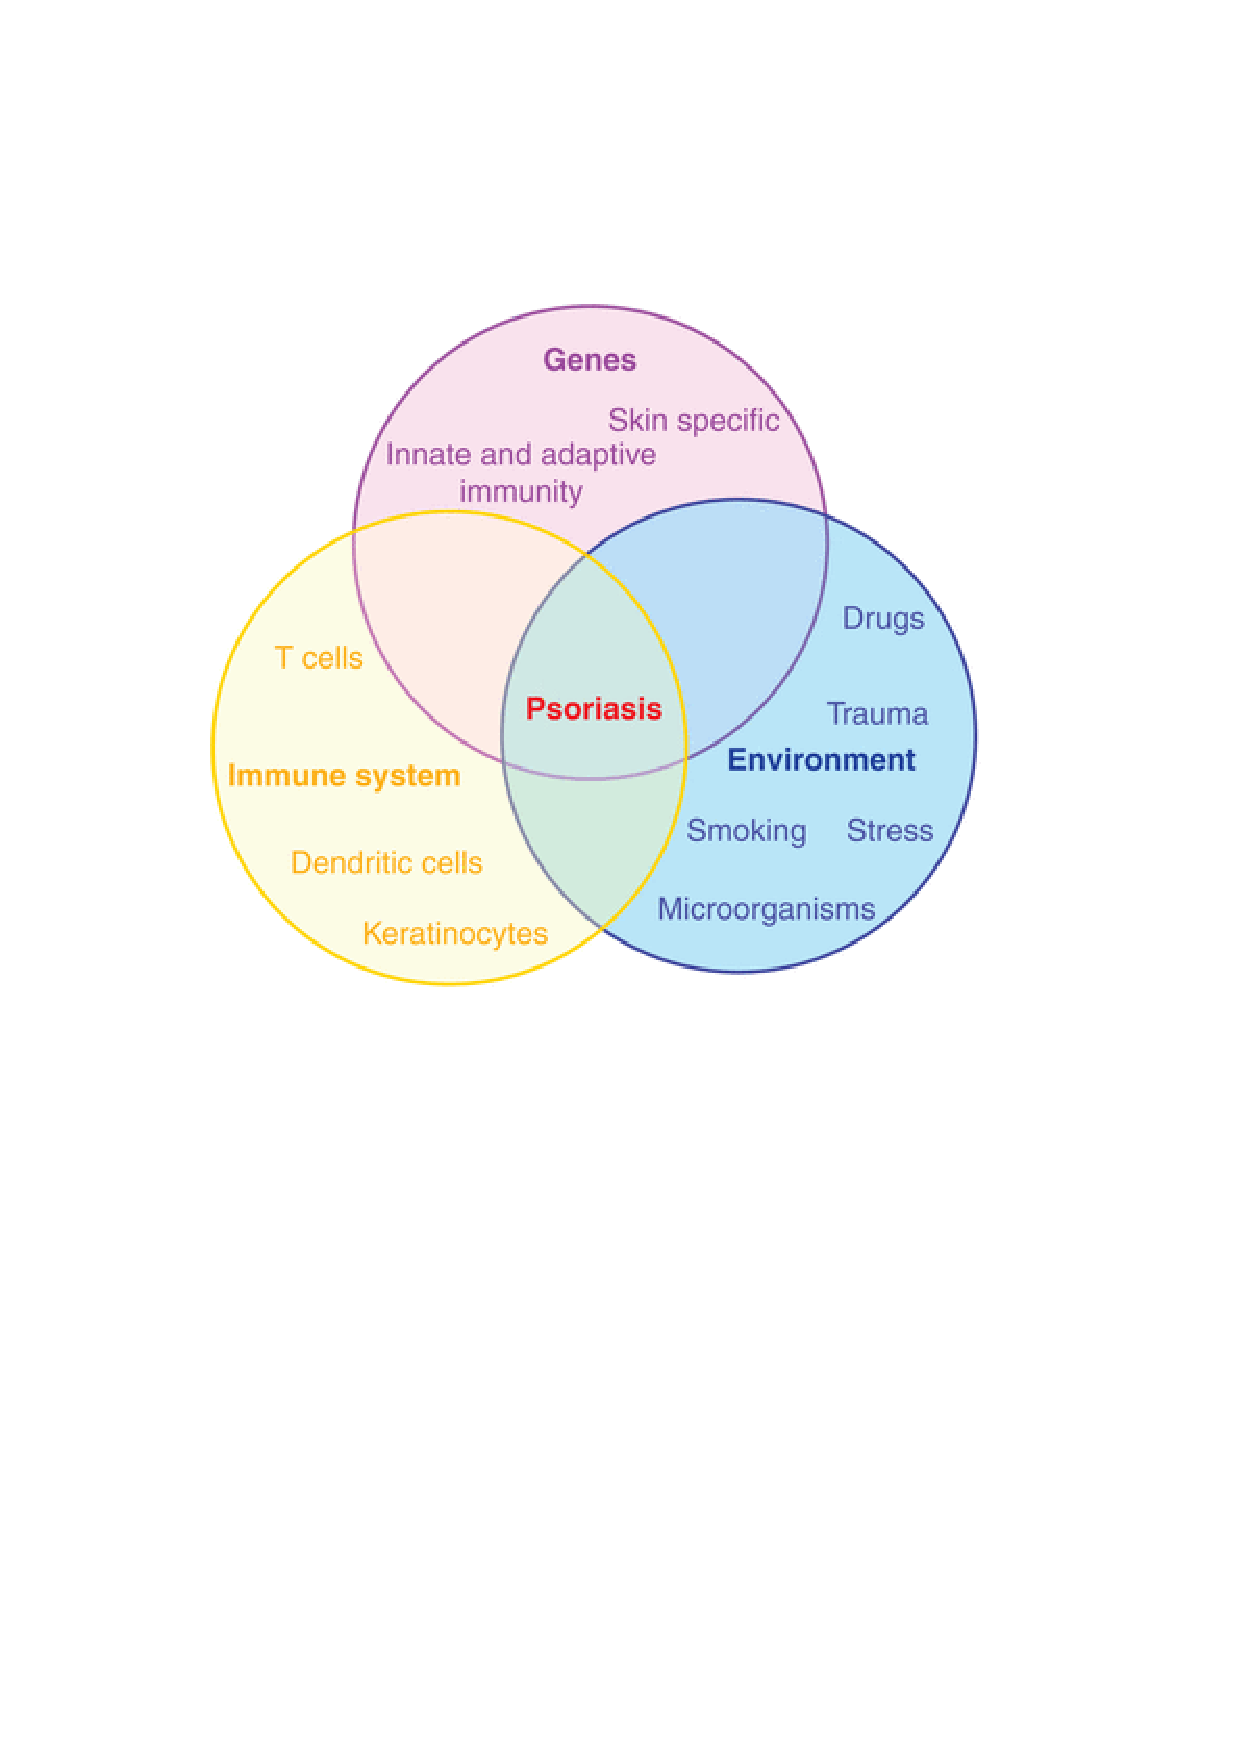
\includegraphics[width=\textwidth]{./Introduction/pdfs/PSO_aetiology_diagram_Di_Meglio_et_al_2014.pdf}
%\caption[Main factors involved in psoriasis disease aetiology]{\textbf{Figure adapted from \parencite{Meglio2014}}}
%\label{fig:PSO_aetiology_diagram}
%\end{figure}


\subsubsection{Histopathological alterations in skin and joints}

The epidermis is the most external structure of the skin and it is formed by approximately 90\% keratinocytes (KC) organised in a layer structure that self-renews in a time dependent manner from the bottom to the surface \parencite{Wikramanayake2014}. As the KC differentiate they undergo changes in morphology, replication ability and keratin composition of their intracellular matrix. In the context of psoriasis impaired epidermis cell renewal leads histological alterations and development of the psoriatic lesions. KC undergo upregulation in the proliferation rate (hyperplasia) that causes aberrant cell differentiation (parakeratosis) (ref) thickening of the epidermis and the subsequent scale formation (ref). Concomitantly, inflammation causes immune cell infiltration and hypervascularisation of the lesion driven by upregulation in the expression of angiogenic factors and activation of the endothelium \parencite{Perera2012}. 

In PsA, joint affection usually follows skin lesions and it involves a wide range of histological changes in the joints, particularly bone remodeling \parencite{Haddad2013}. One of the most common structural changes is the arthritis caused by the swelling and inflammation of the joints \parencite{Schett2011}. As result of this inflammation, alterations in bone remodeling leads to osteolysis with subsequent bone resorption and erosion at the affected joints \parencite{Mensah2017}. This phenomenon is particularly relevant in arthritis mutilans or chronic absortive arthritis, one of the most severe forms of PsA \parencite{Haddad2013}. Bone erosion is also the main histopathological process driving dactylatis, where bone lysis resolves in shortening of the digits \parencite{Gladman2005}. On the other hand, 35\% of the PsA patients undergo inflammation of the connective tissue at the insertion of tendons or ligaments, phenomenon known as enthesitis \parencite{McGonagle2011,Polachek2017}. Overtime, this causes debilitating structural changes due to formation of bony spurs along the insertion sites\parencite{Schett2011}.


\subsubsection{Dysregulation of the innate and adaptive immune response}
%link to the histological changes
The dysregulated  immune response in psoriasis and PSA is the result of the interaction between innate and adaptive immune cells (ref section) resulting in feedback loops involving a complex cytokine milieu. Among the most relevant cytokines of the innate immunity involved in disease initiation are IFN-$\alpha$ and IFN-$\gamma$ \parencite{Leanne2009}. They are mainly produced by circulating plasmacytoid DC (pDC) and myeloid DC (mDC), respectively, upon activation by KC proinflammatory cytokines \parencite{Perera2012}. Both are upregulated at the mRNA level in the lesional skin and contribute to lymphocyte recruitment and maintenance of DC activation \parencite{Schmid1994}. 

Another key cytokine in this dysregulated inflammatory response is TNF-$\alpha$ which has a prominent role in bone turnover and bone remodeling in PsA \parencite{Mensah2008}. It is produced by activated KC, mast cells but also by adaptive immune cells types, including infiltrated T helper(Th) 1 and Th17 cells infiltrated in the psoriatic lesion and PsA inflamed joints \parencite{Perera2012} and it induces activation of nuclear nactor kappa-light-chain-enhancer of activated B cells (NF-$\kapa$B) signaling pathways (ref). It also activates several kinase signaling pathways as well as cell death programs (ref). In the context of inflammation, NF-$\kapa$B represents a master transcriptional regulator of both, the innate and adaptive immune system that induces expression of proinflammatory cytokines, antiapoptotic genes and genes involved in chronic inflammation maintenance (ref). The importance of this transcription factor (TF) in psoriasis and PsA pathogenesis is reflected by the association with disease of several genetic variants in some of the negative regulators of its proinflammatory activity, including NF-$\kapa$B inhibitor alpha \textit{NFKBIA} and TNF receptor-associated factor 3 interacting protein 2 \textit{TRAF3IP2} (ref).
 
Interleukin-23 (IL23) and Th17 axis represents a key loop for the maintenance of psoriasis and PsA inflammatory response and a very important link between innate and adaptive immunity. IL-23 is an innate regulatory cytokine, mainly produced by mDC and macrophages homing the inflamed skin and it binds to the IL23 receptor (IL23R), which expression is upregulated in the DC and T cells of the lesion and in circulating Th cells (ref). In psoriasis, IL23 is the mediator for the pathogenic loop between activated KC and T cells (ref). Both IL-23 and IL-23R present protective and pathogenic genetic variants associated with psoriasis and PsA risk (ref). The activation of the IL-23 pathway leads importantly to increased IL17 production through NF-\kappaB activation by \textit{TRAF3IP2} (ref). IL17 favors maintenance of the adaptive immune mediated Th17 response through recruitment and activation of neutrophils, induction of proinflammatory cytokines including IL-1\beta and IL-6 and also perpetuation of KC activation (ref) (https://www.ncbi.nlm.nih.gov/pmc/articles/PMC3580541/). % add info
More recently, interleukin 22 (IL22) has arisen as another of the key cytokines in mediating the dysregulated cross talk between the innate and adaptive immune response. IL22 levels are increased in the psoriatic lesions and serum of patients and it is mainly produced by a subset of CD4$^+$ cells known as Th22 (ref). It mediates some of the histological changes in skin as well as AMP production by KC (ref).

% Maybe a paragraph to connect skin and joint affection Identical T cell clonality between skin and synovium https://ac.els-cdn.com/S0198885999000348/1-s2.0-S0198885999000348-main.pdf?_tid=5efa7316-fde5-11e7-8091-00000aacb360&acdnat=1516454913_dd20efb867f822d68d8b09873601e8ad

\subsubsection{Environmental factors and disease}

There are several environmental triggers known to be associated with increased risk and worsening of psoriasis and PsA development. A wide range of drugs including antidepressant, antihypertensive and anticytokine therapies have been clinically associated with initiation, exacerbation and worsening of psoriasis. As examples, therapies such as IFN-\alpha for the treatment of hepatitis C virus and anti-TNF antibodies for the treatment of several chronic inflammatory diseases, including psoriasis \parencite{Kim2010}.

Preceding streptococcal throat infection has likewise been associated with development of type I psoriasis lesions only \parencite{Gudjonsson2003}. This is partially explained by the molecular mimicry found for several streptococcal antigens, such as the M protein (highly similar to the structure of certain human keratins) and bacterial peptidoglycans \parencite{Valdimarsson2009}. Also, there is evidence of homologous T cell clones homing tonsils and psoriatic lesions \parencite{Diluvio2006}. Recent studies looking at the microbiome and disease development have also suggested perturbation in the composition of the gut and skin microbiota of psoriasis and PsA patients compared to the controls \parencite{Yan2017}. Consistently with other chronic inflammatory disease such as IBD and AS, these differences in the microbiome could lead to dysregulation of inflammatory pathways in skin and joints through immunomodulation \parencite{Eppinga2014}.

Physical trauma, including tattoos and surgical incisions, has also been associated with the appearance of psoriatic lesions in uninvolved skin as well as joint inflammation in digits \parencite {Nestle2009} due to initiation of the Koebner phenomenon \parencite{Weiss2002}. Lastly, there are several behavioral factors such as smoking, alcohol and stress with suggested with psoriasis and PsA. However, there are not consistent conclusions of their involvement in triggering disease \parencite{Meglio2014}.

\subsection{Cell types involved in psoriasis and PsA pathogenesis}
%Global report on psoriasis, 2016

There is great debate about the most relevant cell types contributing to psoriasis and PsA pathogenesis. Progressively, both are understood as dynamic and continuous processes where different cell types became predominantly important at different stages of the pathology. Regarding levels of circulating immune cells, severe psoriasis patients (PASI>12) showed significantly decreased numbers of PBMC compared to moderate (PASI<12) and healthy individuals \parencite{Langewouters2008}.
;
KC are one of the most relevant cell type at early stages of psoriasis pathogenesis. Several studies have shown the role of KC as immune sentinels through antigen presentation and production of antimicrobial peptides (AMP), cytokines and chemokines. There is evidence of complex formation between the cationic AMP cathelicidin or LL-37 and self-DNA/RNA released by the damaged KC in the psoriatic skin upon trigger by environmental factors \parencite{Lande2007}. It leads to initiation of the skin inflammation through activation of skin-resident DC \parencite{Nestle2005} and secretion of pro-inflammatory cytokines, importantly IL-1, IL-6 and TNF-$\alpha$, that reinforce activation of DC and Th lymphocytes \parencite{Feldmeyer2007, Arend2008, Nestle2009}. Moreover, expression of the MHC-II allows KC to act as APC and activate memory CD4$^+$ and CD8$^+$ T cells inducing a recall immune response \parencite{Black2007}. Studies in mouse models have shown development of psoriatic lesions in immunodeficient mice upon human xenotransplant of psoriasis skin only \parencite{Boyman2004}. The importance of KC in psoriasis development is also reinforced by the association with psoriasis risk of genes of the late cornified envelope (LCE) family \parencite{Tsoi2012}. Overall, these findings would support the hypothesis attributing the initiation of the chronic inflammatory response in psoriasis as the consequence of the epidermis dysfunction \parencyte{Proskch2008}. 

mDC and pDC have also been considered important innate immune cells in disease initiation \parencite{Mahil20016}. They are professional APC that induce T cell activation and the subsequent adaptive immune response. The relevance of antigen presentation in disease has been highlighted at the cellular \parencite{Rusell1972, Tiilikainen1980} and also at the genetic level with the psoriasis and PsA GWAS association of HLA-Cw*06:02 and ERAP1 \parencite{Strange2010}, which encodes for an aminopeptidase involved in the trimming of peptide antigens. Although pDC are circulating cells absent in healthy skin, they infiltrate into the lesional and uninvolved dermis of psoriasis lesions \parencite{Nestle2005} and get activated by the aforementionedd self-DNA and LL-37 complex through Toll-like Receptor (TLR)-9 \parencite{Lande2007}. In contrast, quiescent mDC are epidermal resident and upon secretion of IFN-$\alpha$ by pDC a 30-fold increase of mature mDC is observed in lesional skin but not in uninvolved or healthy tissue (ref). Different mDC subpopulation mediate the Th1 and Th17 response as well perpetuation of KC activation through IL-23 production (ref). Studies in immunodeficient psoriasis mice models have shown that blockage of downstream  IFN-$\alpha$ signaling or its production by pDC failed to induce T cell activation and onset of psoriasis \parencite{Nestle2005}. 

Neutrophils are also though to be closely involved in disease initiation through their ability to form neutrophil extracellular traps (NET)that contain host DNA and AMP, particularly LL-37 \parencite{Hu2016}. There is evidence of increased NET formation in peripheral blood and lesional skin of psoriasis patients and they seem to be contributing to pDC and CD4$^+$ T activation \parencite{Hu2016}. Neutrophils have also been identified in recent studies as one of the main sources of IL-17 production in the skin lesions \parencite{Lin2011} and they also release a wide range of proteases which some induce KC proliferation \parencite{Mahil2006}.

In the context of the innate immunity, the involvement of monocytes and macrophages in psoriasis and PsA has not been extensively studied. Resident macrophages in the healthy dermis undergo a 3-fold increase in lesional skin and they are involved in disease development through TNF$\alpha$ production \parencite{Perera2012, Mahil2016}. Different mice models for chronic psoriasiform skin inflammation have shown a key role of macrophage migration into the affected skin and TNF-$\alpha$ production for maintenance of the lesions \parencite{Stratis2006, Wang2006}. Some studies using psoriasis and PsA patients derived monocytes have also highlighted the systemic aspects of both pathologies. Psoriasis PBMC isolated monocytes have shown greater phagocytic and bactericidal activity compare to those from healthy individuals \parencite{Bar-Eli1979}. Later studies have also shown increased circulating intermediate monocytes (CD14$^{+}$ high CD16$^{+}$ high) and monocyte aggregation in psoriasis patients with subsequent enhanced platelet activation and angiogenesis \parencite {Golden2015}. %In PsA, synovial membranes levels of monocytes/macrophage metalloproteinases are comparable to those found in RA joints mediating bone erosion through differentiation of classical monocytes into osteoclasts \parencite{Hitchon2002}.

Historically, T lymphocytes have been considered one of the most relevant cell types in initiation and maintenance of psoriasis and PsA, and GWAS association with MHC-I also supports the role of T cells in disease. Report cases in humans have demonstrated that bone marrow transplantation can initiate or terminate psoriasis and, therefore, the role of bone marrow-derived T cells in disease pathophysiology \parencite{Eedy1990, Gardembas1990}. The percentage of circulating T cells in psoriasis has been reported to be dependent of severity. Different studies have shown reduced number of T cells in moderate-to-severe and severe psoriasis patients when compared to milder phenotypes and healthy controls. Despite this reduction, increased percentage of the memory populations CD4$^{+}$CD45RO$^{+}$ and CD8$^{+}$CD45RO$^{+}$ have been demonstrated in the same individuals\parencite{Lecewicz-Toruń2001,Langewouters2008}. There is still controversy regarding the total CD4$^+$ and CD8$^{+}$ abundance and CD4$^{+}$/CD8$^{+}$ ratios in PBMC, which may be due to the phenotype heterogeneity of psoriasis patients in the different studies \parencite{Lecewicz-Toruń2001,Cameron2003,Langewouters2008}. In PsA, no differences  abundance of circulatings T cells have been identified compared to healthy individuals \parencite{Costello1999}.

In healthy skin, CD4$^{+}$ and CD8$^{+}$ are found in the dermis and epidermis, respectively \parencite{Clark2006,Perera2012} and upon lesion development an increase in activated memory CD4$^{+}$CD45RO$^{+}$and CD8$^{+}$CD45RO$^{+}$ in the respective compartments can be detected as soon as 3 days after its appearance \parencite{Clark2006}, highlighting the importance of the memory population. \textit{In vivo} studies conducted in mice by Boyman and colleagues showed that development of psoriasis following engrafted human pre-lesional skin was dependent of local T cell proliferation and it did not required injection of additional factors \parencite{Boyle2013}. This supports the theory where recruitment of circulating T cells is restricted to the priming event and it is minimal afterward \parencite{Perera2012}. The relative importance of CD4$^{+}$versus CD8$^{+}$ in psoriasis initiation has been tested immunodeficient mice with pre-lesional skin xenografts followed with injection of purified activated T cell populations \parencite{Nickoloff1999}. These observations suggested a model where CD4$^{+}$ but not CD8$^{+}$ T cells where required for the progression of uninvolved to lesional skin in mice. Interestingly, injection of CD4$^{+}$ activated cells was followed by an increase in activated resident CD8$^{+}$ T cells expressing the acute activation marker CD69. It suggest a hypothesis where in the skin CD4$^{+}$ drive signaling for activation of resident T cells and the activated CD8$^{+}$ resident population are the main effector cells. In PsA, CD4$^{+}$ are significantly more abundant than CD8$^{+}$ cells in synovial tissues \parencite{Diani2015}. In contrast, CD8$^{+}$ expressing CD45RO are prevalent in the SF and they are also significantly increased when compared to controls \parencite{Costello1999}.

In addition to memory T cells, the contribution of regulatory T (Treg) cells have also been investigated to some extent due their role in immunosurveillance and self-tolerance in the context of autoimmune disease. Nevertheless, controversial results have been found regarding relative abundance and impaired function \parencite{Perera2012}. 

Based on the cytokine profile, psoriasis and PsA has been demonstrated to be a type 1 Th/Tc disease, where naive CD4$^{+}$ and CD8$^{+}$ cells get activated and proliferate in the presence of IL-12 and IFN-$\gamma$ \parencite{Austin1999,Perera2012}. Later studies also identified additional subsets including Th-17/Tc-17 and Th-22/Tc-22, which are mainly dependent on IL-23 and IL-6 for their activation, respectively \parencite{Mahil2016}. The importance Th17 cells and their IL-17 production has been assessed in skin, joints and blood, where increased IL-17 and also IL-23 mRNA and protein levels have been found in psoriasis and PsA patients compared to controls \parencite{Cai2012, reference for joints}. It has been shown that the predominant CD8$^{+}$ cells in the SF are  also IL-17 producers and their abundance correlates with markers of inflammation and structural changes in the joint \parencite{Menon2014}. This finding distinguishes PsA from other forms of arthritis such as RA and is in line with findings on skin that suggest a prominent role of CD8$^{+}$ IL-17 producing cells in the different stages of both pathologies. There is also evidence of the synergistic interaction between Th1 and Th17 cells which overall enhances the production of AMPs by KC \parencite{Kryczek2008}. Understanding of the importance of IL-17 has also led to the discovery of other immune cells producing this pivotal cytokine including innate immune lymphoid (ILC) cells and $\gamma$$\delta$ T cells which have also started to been investigated in the context of psoriasis and PsA pathophysiology and treatment \parencite{Meglio2014,Leijten2015}.
IL-17 producing cell have also been hypothesised to be responsible for the link between skin and joint lesions. Although the precise mechanisms for transition between psoriasis and PsA is unknown, studies using psoriasis and RA mice models have shown that skin lesions facilitate arthritis and joint inflammation % \parencite{}. 
It has been hypothesised that the presence of IL-17 producer cells in inflamed skin located nearby the enthesis of joint under physical stress could trigger the development of PsA.

\begin{figure}[H]
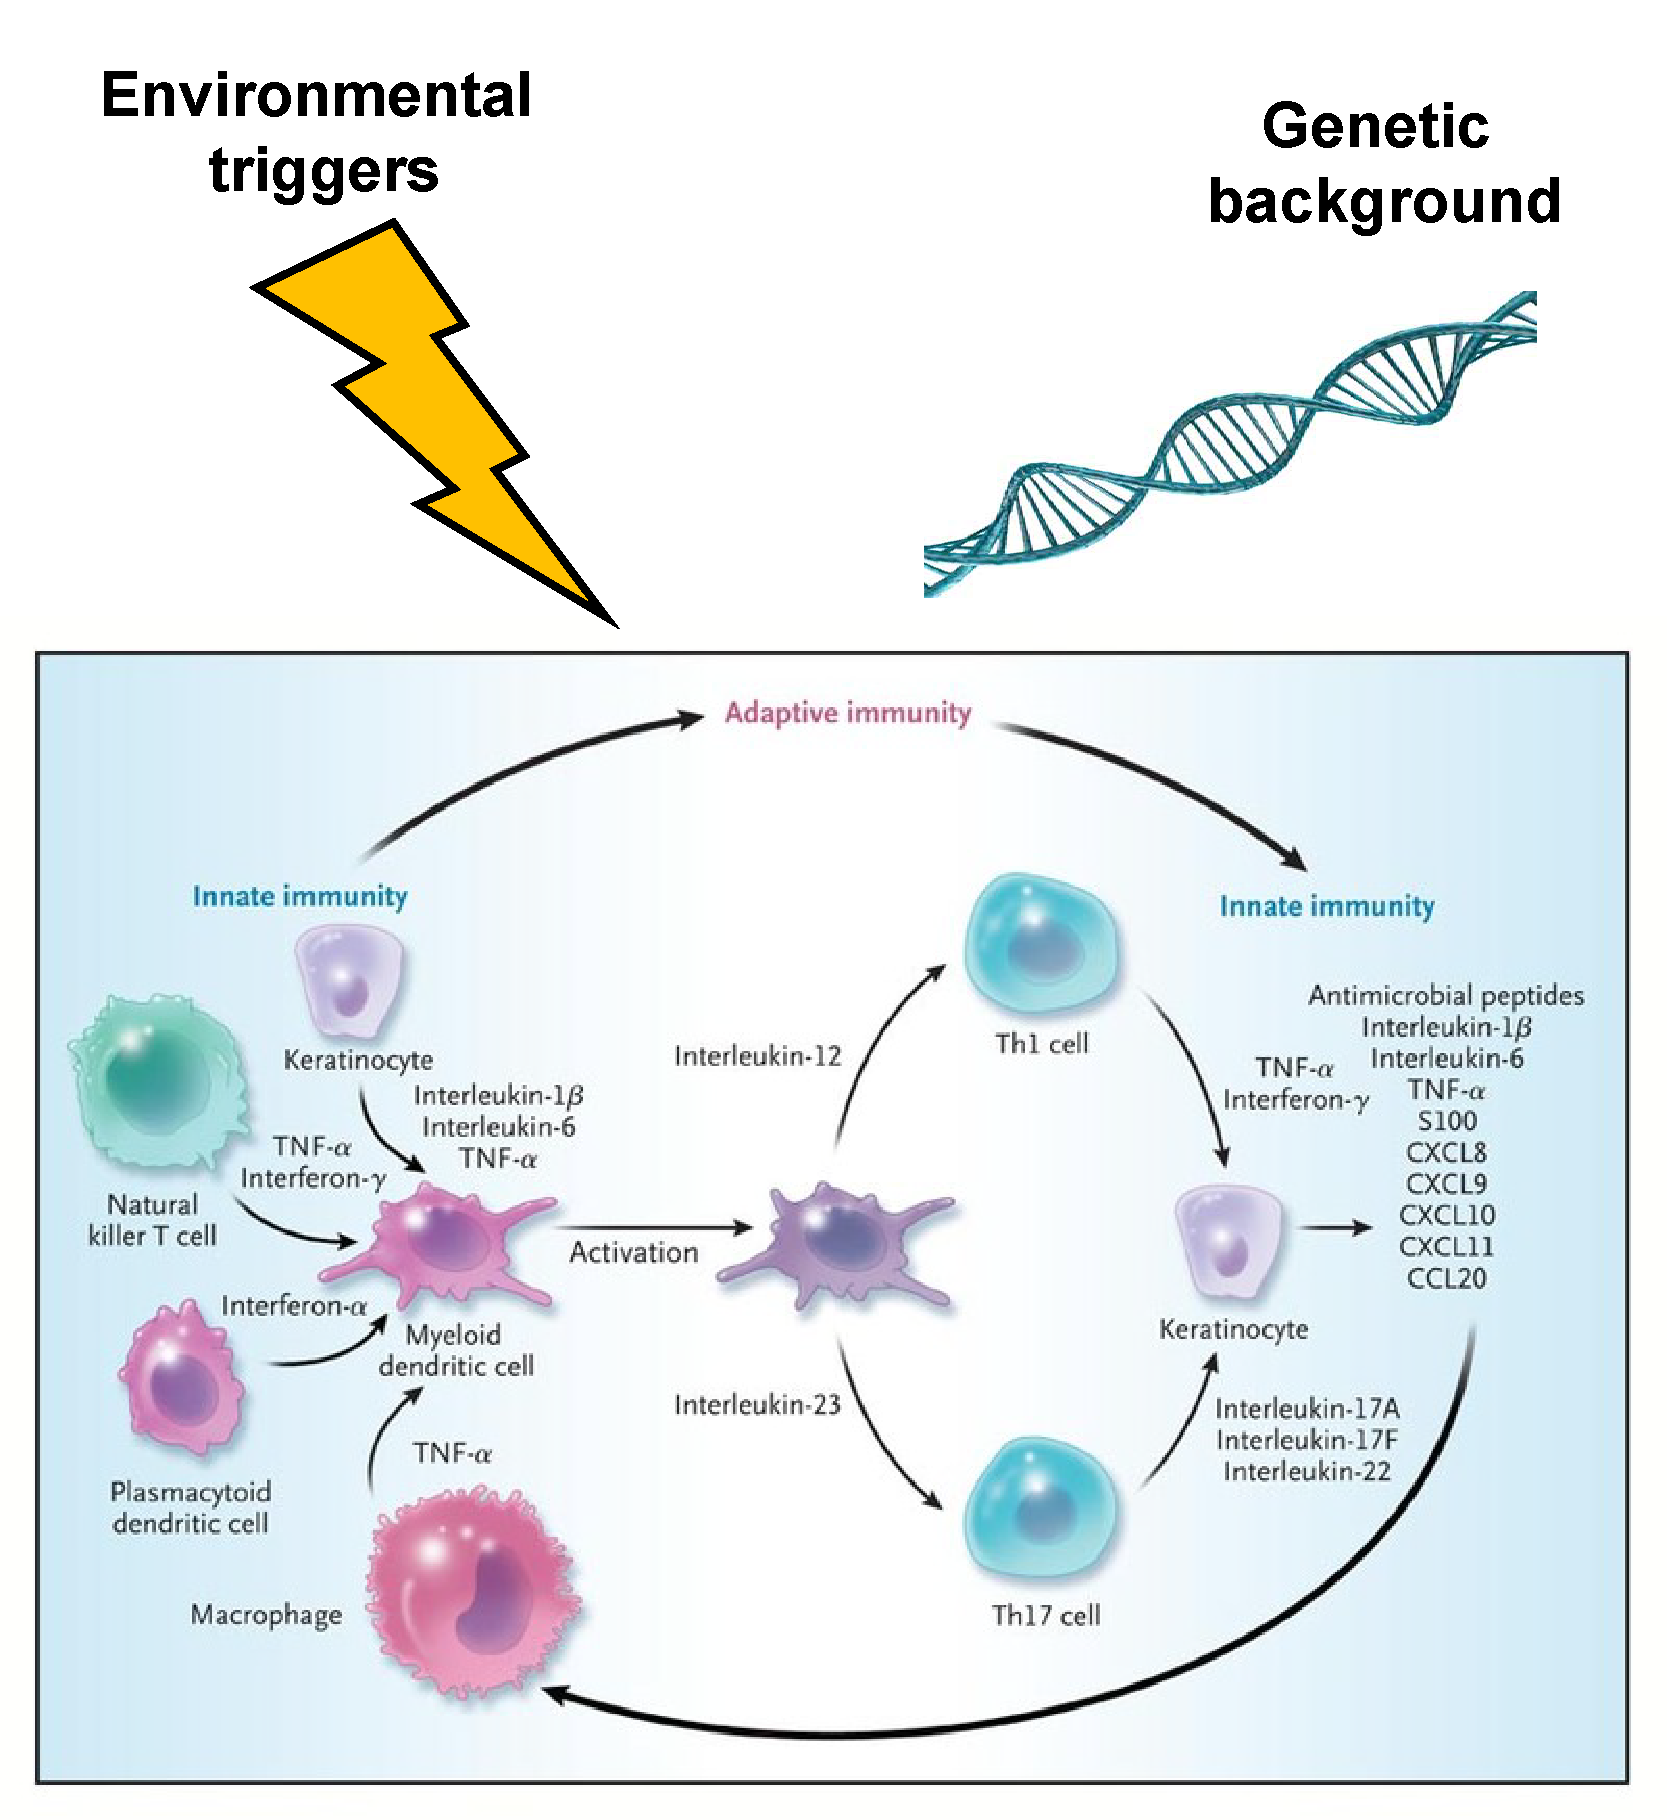
\includegraphics[width=\textwidth]{./Introduction/pdfs/PSO_adaptive_innate_immune_system_crosstalk.pdf}
\caption[Crosstalk between innate and adaptive immunity in psoriasis]{\textbf{Figure adapted from \parencite{Nestle2009}}}
\label{fig:PSO_immune_system_diagram}
\end{figure}

\subsection{Therapeutic intervention and prognosis}

Currently, there is no cure for either psoriasis or PsA and the different treatments available are focused in managing the disease manifestations and symptoms. The approach to treat them are usually dependent on the disease severity. Cases of mild-to-moderate psoriasis are usually managed with topical and systemic therapies \parencite{Menter2009}. Among the topical agents, corticosteroids and emollients are the most commonly used and affordable ones. Emollients are non-medicated agents that contribute to keep the skin soft and moist minimising the symptoms of itching and tenderness and they have been accepted as an adjunctive for the treatment of psoriasis. On the other hand, cortocosteroid in creams, shampoo and spray remain as the most widely spread medical topical treatment due to their antiinflammatory, antiproliferative, and immunosuppressive actions. Corticosteroids are classified based on the potency and they all exert their effect through binding to intracellular corticosteroid receptors and regulation of gene transcription \parencite{Tadicherla2009}. Although they are the most common way to treat mild forms of disease, some of them are approved only for short term treatments as side effects have been reported at a local and systemic level \parencite {Menter2009}. In the case of PsA presenting swelling of two or less joints intraarticular injection of glucocorticosteroids together with joint aspiration have shown to reduce pain and inflammation as a short-time measure \parencite{Coates2016}.    

For psoriasis, other topical treatments are used in combination with topical corticosteroids including ultra violet (UV) light therapy and vitamin D analogues, which inhibit KC proliferation, stimulate KC differentiation and inhibits T cell proliferation and other inflammatory mediators \parencite{Rizova2001}. Topical retinoids and calcineurin inhibitors are also used less frequently for the treatment of psoriasis and they have shown reduced systemic absorption and better suitability for long term treatments in some studies \parencite{Weinstein2003, Menter2009}.

Treatment of most forms of PsA and more moderate-to-severe psoriasis require the use of a broad range of systemic therapies. For mild cases of PsA with involvement of less than four joints and non radiological evidence of structural changes, nonsteroidal antiinflammatory drug (NSAID) are the most commonly used to help controlling the mild inflammatory symptoms and also helping to alleviate the pain and stiffness \parencite{Coates2016}. However, the use of NSAID is not recommended in patients presenting CVD comorbidities due to the increased risk associated with the use of these drugs \parencite{Bhala2013}. For those NSAID-resistant or more severe forms of PsA, disease-modifying antirheumatic drugs (DMARDs) including the an antagonist of folic acid methotrexate (MTX) and the phosphodiesterase 4 inhibitor apremilast have shown to immunosupressive effects on activated T cells and reduction of cytokine production, respectively \parencite{Schmitt2014, Gossec2016, Keating2017,Polachek2017}. However, increased risk of hepatotoxicity for the MTX \parencit{Menter2009} and gastrointestinal side effect  of apremilast \parencit{Menter2009} require requires ensuring appropriate dosing and surveillance. 


The use of biologic systemic agents tend to be the most specific but also expensive treatment for severe cases of psoriasis and PsA and they are not used as the first-line of treatment. These are molecular species generated in cell-based that modulate the immune response in a physiological based manner \parencite{Perera2012}. Among the biologic agents targeting cytokines, TNF$\alpha$ inhibitors (TNFi) have been broadly used for the past five decades to treat both, psoriasis and PsA since this is a pivotal cytokine in initiation and perpetuation of the inflammatory response. There are three TNFi approved for the treatment of psoriasis etanercept, infliximab and adalimumab \parencite{Ahil2016} and another two, certolizumab pegol and golimumab, also used in the management of PsA and other rehumatoid diseases  \parencite{Coates2016b}. All the TNFi are antibody-based agents but etanercep, that is a soluble receptor, and they also show differences in the frequency and via of administration as well as the efficacy, particularly in the specific improvement of skin or joint lesions \parencite{Mease2000}. Although TNF-$\alpha$ blockade is one of the most effective treatments some patients experience common side effects such as increased risk of infection, reactivation of latent infections, demyelinating disease and induced pustular psoriasis have been identified \parencite{Nickoloff2004}. Between 20 to 50\% of the patients fail to respond to the first TFNi and require switching to a second or third one \parencite{Abramson2016}. Lately, new biologic therapies have been developed to target other key cytokines in the pathogenesis of PsA and psoriasis, such as IL-12, IL-23 (ustekinumab) or  IL-17 (secukinumab and ixekizumab) \parencite{Mahil2016}. These new biologics represent a substantial benefit for treating patients and they are routenely administered to individuals failing to respond after a switch to a second TNFi \parencite{Coates2016b}.
 

indirect evidence mDC also produce interleukin 12 (IL12) that could contribute to IFN-$\gamma$ production in lesional skin and inflammed synovium (ref). 

%\subsection{GWAS and functional genomics of psoriasis and other complex diseases}
%\textbf{HLA-C*06:02 mediated pathogenesis}
%The association of the allele HLA-C*06:02 with PSO was first established through serological studies \parencite{Rusell1972, Tiilikainen1980} and it was later on confirmed the association of the region through genetic studies (Ellinghaus et al., 2010; Strange et al., 2010; Stuart et al., 2010; Sun et al., 2010)
%
%the  identification of the precise gene within the associated region of the genome is challenging. Although some earlier studies using microsatellites as markers excluded HLA-C, later genetic studies using dense genotyping that allows better haplotype definition have confirmed HLA-C*06:02 as the susceptibility allele and have identified a single nucleotide polymorphism (SNP) within the gene to drive the greatest association  to disease \parencite{Nair2006, Nair2009} showing 10-fold increase of PSO risk in homozygosis \parencite{Perera2012}
%
%
%number of HLA-C alleles 2375 encoding for 1677 proteins \parencite{Robinson2013}. Particularly, HLA-Cw*06 has 51 different subtypes 
%Regarding allele frequency it changes among ethnic populations. 5553 British Caucasian individuals from the OBB HLA-C allele of greater frequency was HLA-C*07:01 (High resolution HLA haplotyping by imputation for a British population bioresource Neville2017)
%
%
%
%Association of HLAC with other diseases such as Hepatitis C, PsA, primary sclerosing cholangitis and Grave´s disease \parencite{Blais2011}
%
%However, the detailed role of HLA-C*06:02 in the pathogenesis of PSO remains uncertain partly due to the homology between different MHC-In and the polymorphic nature of HLA-C. 
	%Presence of SNPs in minimal promoter and enhancer region that affects expression levels of HLA-C alleles \parencite{Clop2013, Hundhausen2012}. However HLA-Cw*0602 transcript levels do not differ significantly between normal and psoriatic showing responsiveness to proinflammatory cytokines and suggesting the association is not explained by alteration in regulation of gene expression \parencite{Hundhausen2012}. 
	%Lack of functional studies showing specific antigen or interacting proteins recognised by this allele
	%
%HLA-C is  is a heterodimer consisting of a heavy chain and a light chain and expressed in the surface of most of the cells, including antigen presenting cells (APC); however it has lower expression levels and degree of polymorphism than HLA-A and HLA-B ( Low HLA-C expression at cell surfaces correlates with increased turnover of heavy chain mRNA).
%
 %The major role of HLA-C has been assumed to be in acting as a ligand for killer immunoglobulin receptors (KIRs) expressed on natural killer (NK) cells however it is also recognised by TCR of CD8+ cells, not being clear if it exerts its pathogenic role through T cell or NK regulation 
%APC can activate immune response through presentation of processed antigens to CD8+ T cells, very abundant in the lesional epidermis due to inflitration that antigen could be T cell recognition of self-peptides hypothesis reinforced by epistasia with ERAP1 \parencite{Strange2010}, which encodes for an aminopeptidase involved in the trimming of peptide antigens. ERAP1  locus  is  only  associated  with  PSO  in  individuals carrying the HLA-C risk allele. The presentation of autoantigens(Although there are some studies regarding the self-tolerance and presence of autoantigenes as disease trigger \parencite{Lande2007}, the autoimmune aetiology of PSO is still under debate) to CD8+ T cells that clonally expand in psoriasis lesions has been reinforced by the observation of melanocytes as skin-specific target cells of an HLA-C*06:02-restricted psoriatic T cell response. We found that a CD8+ TCR, which we had reconstituted from an epidermal CD8$^+$ T cell clone of an HLA-C*06:02-positive psoriasis patient specifically recognises HLA-C*06:02-positive melanocytes. we observed numerous CD8$^+$ T cells in psoriasis lesions attacking melanocytes, the only epidermal cells expressing ADAMTSL5. Furthermore, ADAMTSL5 stimulation induced the psoriasis signature cytokine, IL-17A %reinfoce 
%, in CD8$^+$ T cells from psoriasis patients only, supporting a role as psoriatic autoantigen. % fact that CD4 are not reactive to autoantigen and that they are the first infiltrated cell type
%This unbiased analysis of a TCR obtained directly from tissue-infiltrating CD8$^+$ T cells reveals that in psoriasis HLA-C*06:02 directs an autoimmune response against melanocytes through autoantigen presentation. We propose that HLA-C*06:02 may predispose to psoriasis via this newly identified autoimmune pathway \parencite{Arakawa2015}.
%
%HLA-Cw*06:02 can be recognised by the inhibitory receptor KIR2DL1 and the activatory receptor KIR2DS1.  Some studies have shown KIR2DS1 was present in 85\% of the patients but only in 51\% of the controls
%NK cells are important regulators of immune responses \parencite{Luszczek2004}. Their function extends beyond killing of infected or transformed cells. Interactions with dendritic cells, macrophages, and fetal trophoblast cells can regulate NK cell activity by influencing cytokine production, cytotoxicity and stimulation of T helper-1 responses. 
%
%
%A similar inflammatory skin phenotype, which was also shown to be T-cell-dependent (Breban et al., 1996), was seen in rats transgenically expressing high levels of HLA-B27 and human β2-microglobulin (Tg(HLA-B*2705, B2M)33-3Trg; Table S1). However, these animals also developed multisystem inflammatory disease characterized by arthritis and colitis (Hammer et al., 1990).
%
%
%
 %
%
   %
%
%
%
%
%Nevertheless, other studies have demonstrated development of PSO in wild type mice upon bone marrow transplantation from mice with PSO-like phenotype
%
%
%
%
%
%
%\subsubsection*{Epigenetics and gene expression}
%\textbf{Understanding the chromatin landscape}
%\textbf{Chromatin accessibility}
%\textbf{Histones modifications}
%\textbf{Understanding the chromatin landscape}
%\textbf{Transcription factor occupancy}
%\textbf{Chromatin interaction}
%
%
%% For later when talking about cohort Approximately one third of patients have moderate to severe disease, which affects more than 10 % of body surface area, and usually necessitates systemic medications.	
\chapter{Material and Methods}
\label{ch:Mat}


%%%%%%%%%%%%%%%%%%%%%%%%%%%%%%%%%%%%%%%%%%%%%%%%%%

\section{Ethical approval and recruitment of study participants}
Sample recruitment for the two different phenotypes and the healthy volunteers were conducted under different ethics.

\subsection{Psoriasis patient recruitment}

Patient blood samples and normal or psoriatic skin biopsies were collected in collaboration with the Dermatology Department research nurses at the Churchill Hospital, Oxford University Hospitals NHS Trust and Professor Graham Ogg at the Weatherall Institute of Molecular Medicine, University of Oxford under approval from the Oxfordshire Research Ethics Committee (REC 09/H0606/71 and 08/H0604/129). After written informed consent, up to 60 mL of blood from eligible psoriasis patients were collected into 10 mL anticoagulant EDTA-containing blood tubes (Vacutainer System, Becton Dickson).

Psoriasis patients were eligible for recruitment when meeting the following criteria:
\begin{itemize}
  \item over 18 years old
  \item previously or newly diagnose, in a flare and going into biologic therapy for the first time % check with Graham
	\item fulfillment of the clinically accepted Psoriasis Area and Severity Index (PASI) classification for psoriasis diagnosis \parencite{Fredriksson1978}
	\item moderate to severe disease (PASI>5) % check with Graham
	\item less than 2 weeks without antibiotics unless used for prophylaxis % check with Graham or research nurses
	\item available clinical information and written consent
\end{itemize}

Detailed clinical information of the psoriasis cohort is included in %(Chapter \ref{ch:})(Table \ref{tab:}).

\subsection{PsA patient recruitment}
Sample recruitment was performed as part of the Immune Function in Inflammatory Arthritis (IFIA) study established in 2013 (REC/06/Q1606/139)in collaboration with research nurses at the Nuffield Orthopaedic Centre, Oxford University Hospitals NHS Trust and Dr Hussein Al-Mossawi at the Botnar Research Centre. Following informed written consent, blood (30 mL) and synovial fluid aspirate (variable upon disease severity) were recruited into 10 mL anticoagulant sodium heparin coated tubes (Vacutainer System, Becton Dickson).

Eligibility of the PsA patients was upon fulfillment of the following criteria:
\begin{itemize}
  \item over 18 years old
  \item previously or newly diagnose, with concomitant psoriasis, in a flare and going into biologic therapy for the first time % check with Hussein
	\item fulfillment of the clinically accepted PsA Response Criteria (PSARC) including a physician global assessment questionnaire \parencite{Philipp2011,Clegg1996}
	\item oligoarticular phenotype and na\"{i}ve for any treatment
	\item less than 2 weeks without antibiotics unless used for prophylaxis % check with Hussein
	\item available clinical information and written consent
\end{itemize}

Further details about the cohort and clinical information can be found in (Chapter \ref{ch:})(Table \ref{tab:}).

\subsection{Healthy volunteer recruitment}
Recruitment of healthy volunteers was conducted as part of the study Genetic Diversity and Gene Expression in White Blood Cells with approval from the Oxford Research Ethics Committee (REC 06/Q1605/55). Up to 80 mL of blood were collected into 10 mL anticoagulant EDTA-containing blood tubes, similarly to the psoriasis sample recruitment.

The criteria for healthy individuals to participate in the study was:
\begin{itemize}
  \item over 18 years old and preferably British or European
  \item no family history of psoriasis, PsA, RA or SpA
	\item matched sex and age with the psoriasis cohort
	\item less than 2 weeks since last infectious process
	\item available clinical information and written consent
\end{itemize}


\section{Sample processing}
\label{sample_processing}
Blood, synovial fluid and skin biopsies were processed straight after recruitment following the appropriate protocols.

\subsection{PBMC and synovial fluid cells isolation}
PBMC were isolated from blood samples through density gradient separation using Ficoll-Paque. Total synovial fluid (SF) cells (SFC) were isolated by centrifugation at 500g for 5 min. Both were washed twice in Hank’s balanced salt solution without calcium or magnesium (Thermo Fisher Scientific) and resuspended in phosphate saline buffer (PBS, Gibco) supplemented with 0.5\% fetal calf serum (FCS, Invitrogen) and 2mM ethylenediaminetetraacetic acid (EDTA, Sigma)prior to cell types separation. Cell numbers and viability were determined by manual count using a haemocytometer and trypan blue (Sigma).

\subsection{Primary cell isolation using magnetic-activated cell sorting}
For the work related to psoriasis and healthy volunteers, primary cell subpopulations were separated using magnetic-activated cell sorting (MACS, Miltenyi). Positive selection was performed for consecutive isolation of CD19$^{+}$ B cells, CD8$^{+}$ T cells, CD14$^{+}$  monocytes and CD4$^{+}$ T cells with AutoMACS Pro (Miltenyi) and cells were manually counted as previously described. MACS separation was chosen over Fluorescence-associated cell sorting (FACS) due to time and logistic constrains in the sample processing and therefore cell numbers in down stream application may not be as exact.

\subsection{Primary cell isolation using fluorescence-activated cell sorting}
Primary cell subpopulations from controls to study the effect of cryopreservation in chromatin states (Chapter 3) or PsA blood and SF samples were isolated by FACS. PBMC and SFC were resuspended in PBS 1mM EDTA (FACS buffer) at 10x10$^6$ cells/mL, stained with the appropriate antibody cocktail (Table \ref{tab:FACS_antibodies}) for 30 min at 4{$^\circ$}C, washed with FACS buffer and centrifuged at 500g for 5 min at 4{$^\circ$}C. For the samples used in Chapter 3, a modified FACS buffer supplemented with 3 mM EDTA , 2\% FCS and 25mM 4-(2-hydroxyethyl)-1-piperazineethanesulfonic acid (HEPES, Invitrogen) was used to avoid cell clumping after cryopreservation and short recovery.After removing the supernatant, cells were resuspended in FACS buffer prior to separation. 

In the controls samples of Chapter 3 only CD14$^{+}$ monocytes and CD3$^+$ CD14$^{-}$ CD4$^{+}$ T cells were isolated in the SONY SH800 cell sorter. For the PsA samples, separation of  CD19$^{+}$ B cells, memory T cells (CD3$^{+}$ CD14$^{-}$ CD4$^{+}$ CD45RA$^{-}$ and CD3$^{+}$ CD14$^{-}$ CD8$^{+}$ CD45RA$^{-}$) ,CD14$^{-}$ monocytes and CD56$^{-}$ NK was performed using FACS Aria (BD) cell sorter from both PBMC and SFC. Bulk sorted cells were collected in 1.5mL tubes in PBS 1\% FCS, whilst single cell and small bulk sorting was performed in 96-well plates in the appropriate buffer (See RNA-seq section). Different nozzle sizes were chosen for bulk and single-cell sorting and OneComp eBeads (eBioscience) were used for compensation of fluorescence spill over.


\begin{table}[htbp]
%\setlength{\tabcolsep}{20pt} only to stretch the columns if you want
%\renewcommand{\arraystretch}{1.5}
\begin{tabular}{@{} c c c c c}
\toprule
\textbf{Surface} & \textbf{Fluorochrome} & \textbf{Manufacturer} & \textbf{Clone} & \textbf{Dilution} \\
\textbf{marker} & \textbf{PsA/CTL} & \textbf{PsA/CTL} & \textbf{PsA/CTL} & \textbf{PsA/CTL} \\
\midrule
\midrule
Viability & eFluor780 & - & eBioscience & 1:250\\
CD3 & FITC/AF700 & SK7/UCHT1 & BioLegend & xxx/1:50\\
CD4 & APC & RPA-T4/RPA-T4 & BioLegend & 1:50/1:50\\
CD8a & PE & RPA-T8 & BioLegend & xxx\\
CD45RA & BV421 & HI100 & BioLegend & xxx\\
CD19 & PerCP-Cy5.5 & SJ25C1 & BioLegend & xxx\\
CD14 & Pe-Cy7/FITC & M5E2/TUK4 & BioLegend/Miltenyi & xxx/1:100\\
CD56 & BV510 & NCAM16.2 & BD & xxx\\
\bottomrule
\end{tabular}
\medskip %gap
\caption[Antibody panel used for FACS separation of primary cell populations in controls and PsA samples]{\textbf{Details regarding target molecule, fluorochrome, clone, supplier and dilution used for PBMC and SFC staining are provided for each of the antibodies in the panel. In controls only CD3, CD4 and CD4 markers were used.}}
\label{tab:FACS_antibodies}
\end{table}
\bigskip %bigger space



%Long table example
%\begin{longtable}{ p{.15\textwidth} p{.25\textwidth} p{.2\textwidth} p{.15\textwidth} p{.15\textwidth}}
%\caption[Antibody panel used for FACS separation of primary cell populations in controls and PsA samples]{\textbf{Details regarding target molecule, fluorochrome, clone, supplier and dilution used for PBMC and SFC staining are provided for each of the antibodies in the panel. In controls only CD3, CD4 and CD4 markers were used.}}
%\label{tab:FACS_antibodies} \\
%
%\toprule
%\textbf{Surface marker} & \textbf{Fluorochrome PsA/controls} & \textbf{Manufacturer PsA/controls} & \textbf{Clone PsA/controls} & \textbf{Dilution PsA/controls} \\
%\midrule
%\midrule
%Viability & eFluor780 & - & eBioscience & 1:250\\
%CD3 & FITC//AF700 & SK7/UCHT1 & BioLegend & xxx/1:50\\
%CD4 & APC & RPA-T4(RPA-T4) & BioLegend & 1:50/1:50\\
%CD8a & PE & RPA-T8 & BioLegend & xxx\\
%CD45RA & BV421 & HI100 & BioLegend & xxx\\
%CD19 & PerCP-Cy5.5 & SJ25C1 & BioLegend & xxx\\
%CD14 & Pe-Cy7/FITC & M5E2/TUK4 & BioLegend/ Miltenyi & xxx/1:100\\
%CD56 & BV510 & NCAM16.2 & BD & xxx\\
%\bottomrule
%\medskip %gap
%
%\end{longtable}
%\bigskip %bigger space
%









\subsection{Skin biopsies processing and adherent assay}
KC enrichment from skin biopsies was performed as described in Gutowska-Owsiak and colleagues \parencite{Gutowska‐Owsiak2012}. Skin biopsies (approximately 4mm) were washed with PBS, cut in 1mm width strips and incubated in 2U/mL of dispase II (Sigma) overnight at 4{$^\circ$}C. The epidermis was separated from the dermis and either snap-frozen in liquid nitrogen (for RNA extraction) or further digested in trypsin (Invitrogen) at 37{$^\circ$}C for 5 min, when used for chromatin accessibility assay. After digestion the resulting cell suspension was filtered through a 70$\micro$m nylon strainer (BD) and washed with PBS. In some instances cells were manually counted and aliquoted for ATAC-seq processing. In others, cell from each of the biopsies were resuspended in KGM-2 BulletKit (Lonza) supplemented with 0.06mM Ca$^2{+}$ and cultured in a collagen IV coated 96-well plate at 4{$^\circ$}C for 10 min or 3 hours, upon experimental requirements (see Chapter X). After culturing, cells were washed twice with 200$\micro$L of PBS and kept at 37{$^\circ$}C for downstream processing.



\section{Experimental protocols}
\subsection{Cryopreservation and cell culture}
For the controls samples in Chapter 3, 40-50x10$^6$ of PBMC were freeze-thawing using a modified version of the \parencite{Kent2009} protocol, where cells were pre-conditioned in RPMI 1640 (brand) complete medium supplemented with2 mM L-glutamine, 100U penicillin and strep 100$\micro$g/mL and 50\% FCS for 30 minutes and afterwards diluted 1 in 2 in complete RPMI 1640 (supplemented as previously described) with 20\% dimethyl sulfoxide (DMSO, Sigma). PBMC underwent slow cryopreservation at -80{$^\circ$}CC in isopropanol at -1{$^\circ$}C per minute and stored for a minimum of two weeks in liquid nitrogen. PBMC were thaw, resuspended in supplemented complete RPMI 1640 with 10\% FCS at a density of 10$^6$ cells/mL and rested for 30 min at 37°C, 5\% CO2 in 25mL non-adherent polypropylene cell culture flasks followed by filtering through a 40$\micro$m to obtain an homogenous cell suspension undergoing FACS separation.
%
Frozen Normal human epidermal keratinocytes (NHEK) in passage 3 were recovered and cultured at a cell density of 5x10$^6$ cells/mL in a 75 mL adherent cell culture flask (brand) in EpiLife basal medium (Gibco) following manufacturer's instructions. After recovery NHEK were trypsinised at room temperature for 8 minutes followed by trypsin inactivation with EpiLife 10\% FCS, centrifugation at 180g for 10 min at room temperature and manual counting with trypan blue. NHEK were seeded in a 96-well plate in 100uL of medium at a cell density of 160 cells/$\micro$L. NHEK were cultured for 2 days to a 90-100\% confluence before being used downstream.

\subsection{ATAC-seq, Fast-ATAC and Omni-ATAC}
Improved versions of the ATAC-seq protocol were progressively used in the thesis for assessment of chromatin accessibility in different primary cells, including CD14$^{+}$ monocytes, CD4$^+$ and CD8$^+$ T cells, CD19$^+$ B cells and CD56$^+$ NK cells. The subsequent version aimed to reduce the amount of mitochondrial DNA and improve the ratio of signal to noise for this technique.

After MACS separation, primary cells were manually counted as above specified and they were resuspended in PBS with 1\% FCS. As previously stated, due to reduced accuracy of manual cell counting compared to FACS sorting, in my experiments ATAC-seq was performed using an estimated number of cells between 50,000 to 100,000. ATAC-seq was performed as described in Buenrostro \textit{et al.}, 2013 with minor modifications. Cells were centrifuged at 500g for 5 min at 4{$^\circ$}C. After removing the supernatant cells were lysed for 10 min, the nuclei were transposed using the Nextera Tn5 transposase (Illumina) for 40 min at 37{$^\circ$}C and DNA was purified using the PCR MinElute kit (Qigen). Additional modifications and performance in 96-well plates were implemented for KC and they will be described in %(Chapter \ref{ch:}). 

After appropriate determination of the amount of DNA amplification using qPCR, samples were amplified and singled indexed for 11 PCR cycles using modified Nextera primers from Buenrostro \textit{et al.},2013 (Table\ref{tab:Indexing_primers}). The resulting DNA libraries were purified using the MinElute PCR purification kit  (Qiagen) and additional Agencourt AMPure XP Magentic Beads (Beckman Coulter), according to the manual specifications, to remove the remaining adaptors and primer dimers.

\begin{landscape}
\begin{table}[htbp]
\setlength{\tabcolsep}{20pt}
%\renewcommand{\arraystretch}{1.5} makes it longer
\begin{center}
\begin{tabular}{@{} c c}
\toprule
\textbf{Primer name} & \textbf{Full sequence} \\
\midrule
\midrule
Ad1.noMX & AATGATACGGCGACCACCGAGATCTACACTCGTCGGCAGCGTCAGATGTG \\
Ad2.1 & CAAGCAGAAGACGGCATACGAGAT\textcolor{blue}{TCGCCTTA}GTCTCGTGGGCTCGGAGATGT \\
Ad2.2 & CAAGCAGAAGACGGCATACGAGAT\textcolor{blue}{CTAGTACG}GTCTCGTGGGCTCGGAGATGT \\
Ad2.3 & CAAGCAGAAGACGGCATACGAGAT\textcolor{blue}{TTCTGCCT}GTCTCGTGGGCTCGGAGATGT \\
Ad2.4 & CAAGCAGAAGACGGCATACGAGAT\textcolor{blue}{GCTCAGGA}GTCTCGTGGGCTCGGAGATGT \\
Ad2.5 & CAAGCAGAAGACGGCATACGAGAT\textcolor{blue}{AGGAGTCC}GTCTCGTGGGCTCGGAGATGT \\
Ad2.6 & CAAGCAGAAGACGGCATACGAGAT\textcolor{blue}{CATGCCTA}GTCTCGTGGGCTCGGAGATGT \\
Ad2.7 & CAAGCAGAAGACGGCATACGAGAT\textcolor{blue}{GTAGAGAG}GTCTCGTGGGCTCGGAGATGT \\
Ad2.8 & CAAGCAGAAGACGGCATACGAGAT\textcolor{blue}{CCTCTCTG}GTCTCGTGGGCTCGGAGATGT\\ 
Ad2.9 & CAAGCAGAAGACGGCATACGAGAT\textcolor{blue}{AGCGTAGC}GTCTCGTGGGCTCGGAGATGT \\
Ad2.10 & CAAGCAGAAGACGGCATACGAGAT\textcolor{blue}{CAGCCTCG}GTCTCGTGGGCTCGGAGATGT \\
Ad2.11 & CAAGCAGAAGACGGCATACGAGAT\textcolor{blue}{TGCCTCTT}GTCTCGTGGGCTCGGAGATGT \\
Ad2.12 & CAAGCAGAAGACGGCATACGAGAT\textcolor{blue}{TCCTCTAC}GTCTCGTGGGCTCGGAGATGT \\
Ad2.13 & CAAGCAGAAGACGGCATACGAGAT\textcolor{blue}{ATCACGAC}GTCTCGTGGGCTCGGAGATGT \\
Ad2.14 & CAAGCAGAAGACGGCATACGAGAT\textcolor{blue}{ACAGTGGT}GTCTCGTGGGCTCGGAGATGT \\ 
Ad2.15 & CAAGCAGAAGACGGCATACGAGAT\textcolor{blue}{CAGATCCA}GTCTCGTGGGCTCGGAGATGT \\
Ad2.16 & CAAGCAGAAGACGGCATACGAGAT\textcolor{blue}{ACAAACGG}GTCTCGTGGGCTCGGAGATGT \\
Ad2.22 & CAAGCAGAAGACGGCATACGAGAT\textcolor{blue}{TGTGACCA}GTCTCGTGGGCTCGGAGATGT \\
Ad2.23 & CAAGCAGAAGACGGCATACGAGAT\textcolor{blue}{AGGGTCAA}GTCTCGTGGGCTCGGAGATGT \\
\bottomrule
\end{tabular}
\medskip %gap
\caption[Modified Illumina Nextera indexing primers]{\textbf{Name and full sequence of the PCR primers used for amplification, indexing and pooling of the ATAC-seq and ChIPm samples in this thesis. These primers were designed by Buenrostro \textit{et al.}, 2013 and they are an modified version of the Nextera Illumina primers optimised for larger molecular weight DNA fragments from low input samples. All samples were indexed with the universal primer Ad1.noMx and one of the additional 18 primers. The indexing sequence of each of the primers is in blue text.}}
\label{tab:Indexing_primers}
\end{center}
\end{table}
\end{landscape}
\bigskip %bigger space

Following the Nature Methods publication of Corces et al., 2016, the  initial ATAC-seq protocol was replaced by a modified version named Fast-ATAC. It was specifically optimised for hematopoietic cells and combined cell lysis and transposition in a single step. Fast-ATAC was performed as described by Corces et al., 2016 with minor modifications. Since 5,000 cells was considered the lower limit to generate good quality data in Fast-ATAC, in my experiments I used 20,000 MACS or FACS sorted cells, to account for inaccurate manual cell counting as well as possible cell loss over centrifugation steps. The Fast-ATAC reaction was performed for 30 min at 37{$^\circ$}C and agitation at 400rpm. DNA was purified as in ATAC-seq and libraries were generated following 13 cycles of PCR amplification, following appropriate cell cycle determination. Purification following PCR were performed using Agencourt AMPure XP Magentic Beads only.

Omni-ATAC, a third generation of ATAC-seq was published by Corces et al., 2017. It consisted in an universal protocol with individual cell lysis and transposition reactions intercalated with a washing step, to remove mitochondrial DNA and other cell debri %check. 
Omni-ATAC was performed as described by Corces and colleagues \parencite{Corces2017} using 50,000 cells.

Following either of the three protocols, DNA tagmentation profiles were assessed with the D1000 high sensitivity DNA tape (Agilent) as part of the quality control and quantified using the Kapa kit (Roche), following the manufacturer's instructions. Pools of 12 to 16 libraries were sequenced in one to 3 lanes of the HiSeq4000 Illumina platform by the Oxford Genomics Centre at the Wellcome Trust Centre for Human Genetics to achieve approximately 50 million paired-end reads.


\subsection{Chromatin Immunoprecipitation with sequencing library preparation by Tn5 transposase}
Assessment of histone marks modification in the chromatin of psoriasis patients from Cohort 1B and four age matched healthy volunteers was performed using a low cell input Chromatin Immunoprecipitation (ChIP) method know as ChIPmentation (ChIPm). For each individual and cell type three histone marks, including H3K27ac, H3K4me1 and X were tested in chromatin isolated from 100,000 cells and compared to an input chromatin sample processed in parallel. Samples were processed following the protocol published by Schmidl and colleagues \parencite{Schmidl2015} with some modifications. Aliquots of 600,000 cells of MACS sorted cell types, as described in \ref{sample_processing}, were fixed with 1\% formaldehyde (Sigma) and snap frozen in dry ice and ethanol prior to storage at -80{$^\circ$}C. Chromatin sonications of the different individuals and cell types were performed in one batch using Covaris M220(Covaris). Each of the aliquots was resuspended in 130$\micro$L of SDS lysis buffer (Table\ref{tab:ChIPm_buffers}), sonicated for 8 min using a duty factor of 5\% and aliquoted for single ChIPm reactions prior to long term storage at -80{$^\circ$}C.

Sonicated chromatin aliquots were thawed and 1.5 volumes of ChIP equilibration buffer (Table\ref{tab:ChIPm_buffers}) was added in order to  reduce the SDS concentration to 0.1\% and to achieve the appropriate concentration of NaCl and Triton-X100. For the immunoprecipitation step, samples were incubated with the appropriate amount of antibody (Table \ref{tab:ChIPm_antibodies}) overnight in rotation  at 4{$^\circ$}C . Protein-A Dynabeads (Invitrogen) were also washed in beads wash buffer (Table\ref{tab:ChIPm_buffers}), blocked with yeast tRNA (Ambion) and BSA (NEB) overnight in rotation at 4{$^\circ$}C and added to the sample-antibody mix for incubation. After appropriate washes, tagmentation was performed on the bead-antibody bound crosslinked complexes, which prevents overtagmentation of the DNA. This was followed by protein K digest, reverse crosslinking, elution of the DNA and from the beads and purification using PCR MinElute kit. The chromatin input control samples were quantified with Qbit after reverse crosslinking and 1ng of chromatin was used for tagmentation.

Amplification by qPCR was done in each of the samples and control inputs to identify the number of full cycles required to reach one-third of the final fluorescence. Libraries were amplified for the number of cycles minus one determined with this strategy to minimise the total number of PCR replicates. The primers used for amplification and indexing were the ones optimised by Buenrostro and colleagues (Table\ref{tab:Indexing_primers}). The number of amplification cycles for each of the samples is recorded in %\ref{Table:}.

\begin{table}[htbp]
\begin{tabular}{@{} c c}
\toprule
\textbf{Reagent} & \textbf{Final concentration}\\
 & & \\
\bottomrule
 & \textbf{SDS lysis buffer} & \\
\midrule
\midrule
SDS & 0.25\% & Sigma \\	
EDTA	& 1mM & X \\
Tris-HCl pH 8 & 10mM & Sigma \\
PI & 1X & Roche \\
Water & - \\
\bottomrule
 & \textbf{ChIP equilibration buffer}  & \\
\midrule
\midrule
Triton-X100 & 1.66\% \\
EDTA	& 1mM \\
NaCl	& 233mM \\
Tris-HCl pH 8 & 10mM \\
PI & 1X \\
Water & - \\
\bottomrule
 & \textbf{Beads washing buffer} & \\
\midrule
\midrule
SDS & 0.1\% \\
EDTA	& 50mM \\
NaCl & 150mM \\
NP-40 & 1\% \\
Tris-HCl pH 8 & 10mM \\
PI & 1X \\
Water & - \\
\bottomrule

 & \textbf{ChIP buffer} & \\
\midrule
\midrule
SDS & 0.1\% \\
Triton-X100 & 1\% \\
EDTA	& 1mM \\
NaCl & 140mM \\
Tris-HCl pH 8 & 10mM \\
PI & 1X \\
Water & - \\
\bottomrule
\end{tabular}
\medskip %gap
\caption[ChIPm buffers modified from Schmidl \textit{et. al}, 2015]{\textbf{Composition of the three modified buffers in house for the ChIPm protocol: SDS lysis buffer, ChIP equilibration buffer, beads washing buffer and ChIP buffer. For each of the buffers the reagents, composition and supplier are indicated.The final volume prepared for each buffer was adjusted depending on the number of samples processed at the time. Sodium dodecyl sulfate (SDS), PI (proteinase inhibitor). Supplier for each of the reagents as follows: SDS (Sigma), EDTA(xxx), Tris-HCl pH8 (xx), Triton-X100 (xxx), NP-40 (Sigma) NaCl(xx), PI (Roche) and water (Ambion) }}
\label{tab:ChIPm_buffers}
\end{table}
\bigskip %bigger space

\begin{table}[htbp]
\setlength{\tabcolsep}{20pt}
\renewcommand{\arraystretch}{1.5}
\begin{tabular}{@{} c c c c}
\toprule
\textbf{Histone mark} & \textbf{Feature} &\textbf{$\micro$g per sample} & \textbf{Manufacturer}\\
\midrule
H3K27ac & Active enhancer, promoter & 2 & Diagenode (C15410196)\\
H3K4me1 & Enhancer & 1 & Diagenode (C15410194)\\
H3K4me3 & Active promoter, enhancer & 1 & Diagenode (C15410003) \\
\bottomrule
\end{tabular}
\medskip %gap
\caption[Antibody panel used for immunoprecipitation of histone marks in ChIPm]{\textbf{Details regarding the histone marks, the the most likely chromatin state delineated, the amount of antibody required per reaction and the supplier and catalog num of the antibodies.}}
\label{tab:ChIPm_antibodies}
\end{table}
\bigskip %bigger space


\subsection{RNA extraction and RNA-seq}

\subsubsection{Bulk RNA-seq}
Following MACS isolation of the different cell types from the psoriasis and matched healthy controls, between 2-3x10^6 cells were resuspended in 350$\micro$L of RNAProtect (Qiagen) or RLT buffer (Qiagen) supplemented with 0.1\% of beta-mercaptoethanol (BM, Sigma) and snap frozen in dry ice before storage at -80{$^\circ$}C. Cells isolated from psoriasis and control Cohort 1A (Chapter \ref{ch:}) were preserved in RNAProtect, which stops any biochemical reaction and transcriptional activity maintaining cell integrity. At early stages of the project, when I was uncertain of time frames to process the different material from the acquires samples, I decided to use RNAProtect to preserve cells for future RNA extraction to guarantee high quality in case storage exceeded 6 months. In the psoriasis and control samples from Cohort 1B %(Chapter \ref{ch:}) 
, cells were resuspended in 0.1\% BM supplemented RLT buffer, which lysates cells and prevents RNA degradation. Cell lysates were homogonised using the QIAshredder (Qiagen) prior to RNA extraction. When starting from RNAProtect preserved material, cells were centrifuged at 300g for 10 min at room temperature, the supernatant were removed and the pellets were resuspended in 350$\micro$L of RLT 0.1\% BM buffer, prior to homogenisation with QIAshredder.

Total RNA were extracted using the AllPrep DNA/mRNA/microRNA Universal kit (Qiagen) following the manufacturer's instructions. RNA extractions were performed in batches of 12 samples, including all cell types from each individual and a balanced numbers of psoriasis and control samples, to minimise batch effect correlation with phenotype groups. Basic quantification was performed with NanoDrop (Thermo Scientific) before storage at -80{$^\circ$}C.

RNA-seq quality control (QC), quantification, library preparation and sequencing were carried out by Oxford Genomics Centre at the Wellcome Trust Centre for Human Genetics in two independent batches of samples, each including Cohort 1A or Cohort 1B, respectively. Processing of samples in two batches was due to logistics of patients recruitment in the project. Quality control and quantification were assessed with the Bioanalyzer (Agilent). Preparation of RNA-seq libraries was performed using Ribo-Zero rRNA Removal kit (Illumina), based on ribosomal RNA depletion. Unlike strategies using polyadenylated transcripts selection, this method allowed to preserve non-polyadenylated transcripts including nascent pre-mRNA (unspliced) and functionally relevant lncRNAs. For each of the cohorts, all libraries were pooled together and  sequenced over several lanes of HiSeq4000 to a depth of 50 million total reads per sample in order to maintain an appropriate level of sensitivity for subsequent expression analysis given the greater complexity of these libraries.

 

\subsubsection{PsA memory CD4$^{+}$ and CD8$^{+}$ single-cell RNA-seq} 
\label{scRNA_processing}

Single CD4$^{+}$ or CD8$^{+}$ memory T cells were sorted in 2$\micro$L of cell lysis buffer into 96-well plates. Four and three plates were prepared for CD4$^{+}$ and CD8$^{+}$, respectively, including wells containing 50 cells in each of the plates for control purposes. Libraries were prepared,indexed and sequenced at the Sanger Institute (Cambridge) using the Smart-seq2 methodology as described by Picelli and colleagues \parencite{Picelli2014}. Samples were sequenced using 50-bp single-end Illumina HiSeq2500 at a depth of approximately 4 million reads per cell. %look in notebook for details about scRNA in Cambridge

scRNA-seq was also generated in FACS sorted 1:1 ratio CD4$^{+}$ or CD8$^{+}$ memory T cells and in bulk PBMC using 10X Genomics technology Chromium single cell 3' and 5' expression library prep kits (PN-120267 and PN-1000014, respectively) by the Oxford Genomics Centre at the Wellcome Trust Centre for Human Genetics. Libraries were sequenced with Illumina HiSeq4000 xxxbp single-end at a depth of 50,000 reads per cell.

\subsubsection{Small-bulk RNA-seq } 
Between 100 to 500 cells of the five populations isolated from PsA patients were FACS sorted into 2$\micro$L of cell lysis buffer and processed for library prep as in Picelli \textit{et al.}, 2014 by the Oxford Genomics Centre at the Wellcome Trust Centre for Human Genetics. Libraries were sequenced with Illumina HiSeq4000 xxxx bp single-end at a depth of XXX reads per cell.


\subsection{Single-cell analysis of the V(D)J T cell receptor repertoire}
Single-cell sequencing of the V(D)J segments from TCR transcripts was performed simultaneously with the 10X Genomics technology Chromium 5' expression library kit (PN-1000014) by the Oxford Genomics Centre at the Wellcome Trust Centre for Human Genetics. In short, full-length cDNA was amplified by PCR with primers against the 5’ and 3’ ends of the barcode sequences inherent to the 10X Genomics bead technology. The amplified material was divided for use in 5' total scRNA-seq (as specified previously in \ref{scRNA_processing}) and also for enrichment of the TCR by PCR amplification with specific primers. TCR enriched cDNA was followed by enzymatic fragmentation and size selection in order to obtain variable length fragments spanning the V(D)J segments. Library prep and indexing was followed by Illumina HiSeq4000 xxxx bp single-end sequencing at a depth of XXX reads per cell.

\subsection{DNA extraction and SNP genotyping}
DNA isolation was performed using the AllPrep DNA/mRNA/microRNA Universal kit (Qiagen) following the manufacturer's instructions. Basic quantification was performed using NanoDrop (Thermo Scientific) and kept at -80{$^\circ$}C for long term storage. For each of the patients and controls, the extracted DNA was amplify by PCR using forward (5'-CACTGTGGAGGGAGGAACAA-3') and reverse (5'-CGTGTTGGCCAGGATAGTCT-3')primers annealing up and down stream the SNP rs4672505, respectively. The 390 bp PCR product was purified using MinElute PCR purification kit, quantified by dsDNA Qbit kit (Invitrogen) according to the manufacturer's instructions and prepared for Sanger sequencing using the Mix2Seq service (Eurofins). The forward and reverse sequences were analysed with BioEdit software.



\subsection{Mass cytometry analysis}

Mass cytometry analysis was performed by Dr Nicole Yager in collaboration with UCB following their in-house protocol. Briefly, PBMCs and SFMCs
were split in three ways for 5 min fixation with 1.4\% paraformaldehyde, fixation and 6h treatment with monensin (MN) and brefeldin A (BFA) or fixation and 4h treatment with ionomycin and phorbol-12-myristate-13-acetate (PMA). All samples were treated with cisplatin before fixation to facilitate discrimination of dead cells in the staining. MN and BFA are both inhibitors of protein transport
that prevent the release of cytokines from the cells and allow measuring the intrinsic cytokine production in basal conditions whereas treatment with ionomycin and PMA induces unspecific activation of immune cells. After appropriate treatment, cell suspensions were washed with PBS and stained with a phenotyping panel of forty four cell surface markers (including viability) or permeabilised and stained with the intra-cellular staining (ICS) panel formed by fourty three markers including surface and intracellular targets Table xxxx. Data analysis was conducted using xxxxxx.  

\begin{table}[htbp]
\setlength{\tabcolsep}{20pt}
\renewcommand{\arraystretch}{1.5}
\begin{tabular}{@{} c c }
\toprule
\textbf{Phenotyping panel} & \textbf{ICS panel} \\
\midrule
CD248, CD19, GP38, FAP, CD4, CD8a, IL8, CD16, CD25, IL4, CD123, IL-21,& CD248, CD19, GP38, CD15, CD4, CD8a, CD34, CD16,\\
FceR, IL-17F, IL-2, TNF$\alpha$, IL-17A, IL-10, CD11c, CD14, &CD25, CD154, CD123-CD64, CRTH2, pSTAT5, CD206, CCR6,CD203c,\\  
CD161, IL6, IFN-$\gamma$, GM-CSF, FCeR, CD44, IL-17FF, IL-17AF, CD3, & CYP2D7,CD68, CD14, CD161, CD127, TCR,NKp44, CD27, \\
CD45RO, CD-11b, CD56, HLA-DR, IL-13, CD117, CD45 &  ST2, CD45RA, CD3, CD45RO, CD38-CD90, CD56, HLADR, KIT \\
\bottomrule
\end{tabular}
\medskip %gap
\caption[Molecules targeted by the phenotyping and cytokine production antibody staining panel in PBMCs and SFMCs.]{\textbf{Molecules targeted by the phenotyping and cytokine production antibody staining panel in PBMCs and SFMCs.}}
\label{tab:CyTOF}
\end{table}
\bigskip %bigger space


\section{Computational and statistical analysis}

\subsection{ATAC-seq data analysis}
\label{ATAC_analysis}
ATAC-seq, Fast-ATAC and Omni-ATAC data were analysed using an in house pipeline towards which development I made an important contribution. The pipeline performs single sample data processing and it also builds a combined master list for each of the comparisons of interest to later perform differential analysis. 

\subsubsection{Next generation sequencing data analysis}
NGS data for each of the samples was trimmed for low quality base pairs and Nextera adapter sequences using cutadapt \parencite{} before general QC assessment using fastqc \parencite{}. Trimmed data was alignment to the reference genome built hg19 using bowtie2 \parencite{Langmead2006} and the following parameters -k 4 -X 2000 -I 38 --mm -1, consistently with other publications \parencite{Buenrostro2013, Corces2016}. Samtools \parencite{} was used to remove PCR duplicates reads previously marked with Picard Tools \parencite{} as well as low MAPQ (${<}$30) non-uniquely and non-properly paired reads. The resulting bam file was additional filtered to remove mitochondrial DNA and reads were adjusted by +4 bp in the plus strand and by -5 bp in the minus strand to represent the center of the transposition binding event. Pileup tracks (bigWig files) for visualisation were generated using bedtools genomeCoverageBed where each value represents number of reads per position \parencite{} and the UCSC genome browser bedGraphToBigWig tool \parencite{}.  

\subsubsection{Peak calling and filtering}
Peak calling was performed using MACS2  callpeak \parencite{} and the parametres --nomodel --shift -100 --extsize 200 --p 0.1 --keep-dup all --call-summits and filtered for those overlapping with the blacklisted features from ENCODE project \parencite{}. The --shift and --extsize parameters were set according to the recommendations of MACS2 for DHS and following other ATAC-seq publications \parencite{Buenrostro2015, Corces2016}. The pval cut off for peak filtering was determine for each of the cell types separately. 
For a particular cell type, the bam file of each sample (patients and controls) was partitioned in two (pseudorreplicates) and peak calling was performed in each of them followed by Irreproducibility Discovery Rate (IDR) analysis to assess the percentage of peaks sharing IDR at each corresponding pval. Median of the pval showing the greater percentage across all the samples was used to filter each peak list. Peak summits were replaced by the median of the summits for those with multiple called summits and extended +/- 250bp to create a non-overlapping homogenous 500bp peak list \parencite{Buenrostro2015, Corces2016}. 

Sample quality was determined by the fol-change enrichment of ATAC-seq signal across all the TSS identified by Ensembl, since chromatin is expected to be more accessible at the sites of transcriptional initiation compared to the flanking regions.  

\subsubsection{Combined peak master list and differential analysis}
To perform differential open chromatin analysis a non-overlapping 500bp peak master list was built for each cell type separately by union of all the peaks that were present in at least 30\% of the samples, regardless patient and control group. Reads overlapping each of those peaks were retrieved for each sample using HTSeq-count algorithm \parencite{} to build a combined count matrix. An empirical 95\% confidence cut-off for the number of counts in absent peaks was calculated on the raw count matrix and used to filter out some peaks in the master list before proceeding to differential analysis (\parencite{Xinmin2005,Jonker2014}). Differential analysis was performed using DESeq2 R packaged taking into account paired samples for the PsA analysis or correcting for covariates for the case-control psoriasis analysis (which covariates???)\parencite{Love2014}.
A combined master list for all cell types and tissues (when applicable) was also built following the same strategy, normalised and used for principal component analysis (PCA). 





\subsection{ChIPm data analysis}

\subsubsection{Next generation sequencing data analysis}
ChIPm NGS data from samples and inputs were processed similarly to ATAC-seq (\ref(ATAC_analysis)) for trimming, mapping and filtering with minor modifications. Particularly, MAPQ30 threshold filtering score was lowered to 10 instead of 30. For visualisation of each sample, biWig files with subtracted noise from the input were generated using MACS2 bdgcmp -m subtract and bedGraphToBigWig tools .

\subsubsection{Peak calling and filtering}
Peak calling for each sample was performed accounting for the background in the input samples using MACS2 callpeak --bw 200 --p 0.1 --keep-dup all --call-summits. In this case the average library fragment size(--bw) was used by MACS2 to first empirically find the model that better represent the precise protein-DNA interaction and then calling peaks with statistical confidence (pval) using the input sample
to calculate the local background. Filtering and down stream peak homogenisation was performed similarly to ATAC-seq analysis (\ref(ATAC_analysis)).

Sample quality for H3K27ac and H3K4me3 ChIPm samples was determined by the fold-change enrichment of the histone mark across all the TSS identified by Ensembl, since both marks are enriched at promoters.  

\subsubsection{Combined peak master list and differential analysis}
To perform differential histone modification analysis a peak master list was built and counts at each of the locations were performed as described for ATAC-seq (\ref(ATAC_analysis)). PCA analysis was performed for samples from all cell types and individuals in a combined master list.

Differential analysis



\subsection{RNA-seq data analysis}

\subsubsection{Bulk RNA-seq analysis}
The ribo-depleted RNA-seq data generated was mapped using the aligner STAR \parencite{Dobin2013} against the Gencode hg19 annotation file containing reference chromosomes, scaffolds and assembly patches. The annotation file comprised 2,840,283 gene entities, including lnc-RNAs. Mapping allowed multiple alignments and only retained those with the best score and a miss-match percentage lower than 0.04\%. Duplicates were marked and removed using Picard Tools. The filtered de-duplicated and sorted bam files were used to retrieve counts at each of the genes location of the annotation file using HTSeq-count. Differential gene expression analysis was performed with DESeq2 R package filtering parameters ...........

 




	\subsubsection{Single-cell RNA-seq analysis}

\subsection{Genomic region annotation, pathway enrichment analysis and visualisation}
Annotation of genomic regions and signalling-pathways visualisation were performed with two functionalities of the R package and web-app Atlas and Analysis of systems-biology-led pathways, developed by Dr. Hai Fang and towards which I have made some contribution (manuscript in preparation). ATAC-seq and ChIPm peaks were annotated with gene entities based on publicly available promoter-HiC data in 17 immune cell types \parencite\parencite{Javierre2016}. The interactions were weighted based on the number of cell types for which the same bait-target interaction was reported as well as on the confidence of each of those interaction measured by the CHiCAGO score. This approach integrates the knowledge in the field about regulatory regions affecting the expression of distal genes and was not biased by the physical vicinity to a gene when annotating genomic intervals located at intergenic regions or gene desserts.For visualisation, manually curated KEGG pathways including all the genes for each gene family were colored based on the fold-change from the corresponding differential analysis and highlighted in bold when passing the FDR threshold for significance.

 \subsection{Enrichment analysis for genomic annotation features}
-Includes the ATAC all peaks enrichment for eQTLs 
-ATAC all peaks enrichment for GWAS
-ATAC for TFBS, chromatin annotation segments
GWAS with eQTL and DOCs using xLDenricher with co-localisation and permutation analysis 20,000

\subsection{Statistical fine-mapping}

											% ch:Intro
%\appendix
\addcontentsline{toc}{chapter}{Appendices}
\startcontents
\startlist[appendix]{lof}
\startlist[appendix]{lot}
\printcontents{atoc}{0}{\chapter*{Appendices}}
\begingroup
\let\clearpage\relax
\singlespacing
\printlist[appendix]{lot}{}{\chapter*{List of Tables}}
\printlist[appendix]{lof}{}{\chapter*{List of Figures}}
\endgroup

\chapter{Tables}
\label{app:Tables}

%\section{Additional tables}

\section{Chapter 3 Tables}

\begin{table}[htbp]
%\setlength{\tabcolsep}{20pt} only to stretch the columns if you want
%\renewcommand{\arraystretch}{1.5}
\centering
\begin{tabular}{@{} c c c c c}
\toprule
                   &                    &               & \textbf{TSS enrichment} &     \\
\textbf{Cell type} & \textbf{Condition} & \textbf{CTL1} & \textbf{CTL2} & \textbf{CTL3} \\
\midrule
\midrule
      & Fresh	 & 17.4 & 19.6 & 14.11\\
CD14	& Frozen & 26.3 & 25.2 & 27.1 \\
      & Fixed	 & 2.5  & 16.5 & 22.4 \\
\midrule
      & Fresh	 & 5.3  & 5.6  & 7.7 \\
CD4	  & Frozen & 17.9 & 14.1 & 16.1 \\
      & Fixed	 & 7.9  & 23.0 & 14.3 \\
\bottomrule
\end{tabular}
\medskip %gap
\caption[Enrichment of ATAC-seq reads across the TSS for the CD14$^+$ monocytes and CD4$^+$ samples fresh, frozen and fixed.]{\textbf{Enrichment of ATAC-seq reads across the TSS for the CD14$^+$ monocytes and CD4$^+$ samples fresh, frozen and fixed.}}
\label{tab:Core_ATAC_TSS_summary_table}
\end{table}
\bigskip %bigger space






\section{Chapter 4 Tables}

\begin{table}[htbp]
%\setlength{\tabcolsep}{20pt} only to stretch the columns if you want
%\renewcommand{\arraystretch}{1.5}
\centering
\begin{tabular}{@{} c c c}
\toprule
\textbf{Sample ID} & \textbf{NRF} & \textbf{PBC1/PBC2} \\
\midrule
\midrule
PS2000 CD14	& 77.6	& 0.60/2.5\\
PS2001 CD14	& 84.9	& 0.70/3.0\\
PS2314 CD14	& 81.1	& 0.60/1.8\\
PS2319 CD14	& 79.9	& 0.60/2.2\\
CTL7 CD14	  & 81.1	& 0.65/2.2\\
CTL8 CD14	  & 83.9	& 0.66/2.3\\
CTL9 CD14	  & 80.7	& 0.60/2.3\\
CTL10 CD14	& 83.1	& 0.65/2.1\\
\midrule
PS2000 CD4  & 84.8	& 0.75/3.4\\
PS2001 CD4	& 82.0	& 0.72/2.9\\
PS2314 CD4	& 82.9	& 0.71/2.8\\
PS2319 CD4	& 82.4	& 0.73/3.2\\
CTL7 CD4	  & 78.6	& 0.68/2.5\\
CTL8 CD4    & 81.8	& 0.71/2.9\\
CTL9 CD4    & 81.6	& 0.74/3.3\\
CTL10 CD4   & 77.6	& 0.61/1.9\\
\midrule
PS2000 CD8 & 77.0 &	0.76/4.5\\
PS2001 CD8 & 74.7 &	0.74/4.0\\
PS2314 CD8 & 74.2 &	0.75/4.1\\
PS2319 CD8 & 72.2 &	0.75/4.0\\
CTL7 CD8	 & 32.7 & 0.32/1.5\\
CTL8 CD8	 & 70.1 &	0.70/3.3\\
CTL9 CD8	 & 73.9 &	0.73/3.7\\
CTL10 CD8	 & 68.2 &	0.65/2.9\\
\midrule
PS2000 CD19	& 38.0 & 0.42/1.9\\
PS2001 CD19	& 71.4 & 0.71/3.7\\
PS2314 CD19	& 29.4 & 0.34/1.8\\
PS2319 CD19	& 76.1 & 0.78/4.8\\
CTL7	CD19  & 74.2	& 0.69/3.1\\
CTL8	CD19  & 68.4  &	0.67/3.2\\
CTL9	CD19  & 75.1  &	0.76/4.6\\
CTL10	CD19  & 61.7  & 0.59/2.6\\
\bottomrule
\end{tabular}
\medskip %gap
\caption[Evaluation of ChiPm library complexity for the psoriasis and control chort 1B ChIPm assay.]{\textbf{Evaluation of ChiPm library complexity for the psoriasis and control chort 1B ChIPm assay.} NRF, PBC1 and PBC2 are the three measures used according to the ENCODE standards as referred in Chapter \ref{ch:Mat}. 0.5$\leq$NRF$<$0.8 acceptable; 0.8$\leq$NRF$\leq$0.9 compliant; NRF$>$0.9 ideal; 0.5$\leq$PBC1$<$0.8 and 1$\leq$PBC2$<$3 moderate bottlenecking; 0.8$\leq$PBC1$<$0.9 and 3$\leq$PBC2$<$10 mild bottlenecking.}
\label{tab:ChIPm_PS_CTL_library_complexity}
\end{table}
\bigskip %bigger space

\begin{table}[htbp]
%\setlength{\tabcolsep}{20pt} only to stretch the columns if you want
%\renewcommand{\arraystretch}{1.5}
\centering
\begin{tabular}{@{} c }
\toprule
\textbf{CD14$^+$ monocytes additional enriched pathways in psoriasis} \\
\midrule
\midrule
Generic transcription \\
RNA transport \\
GnRH signalling \\
Ribosome biogenesis in eukaryotes \\
Neurotrophin signaling \\
Spliceosome \\
Autophagy \\
Protein processing in endoplasmic reticulum \\
                        \\
\textbf{CD8$^+$ additional enriched pathways in psoriasis} \\
\midrule
\midrule
Epstein-Barr virus infection \\
RNA Polymerase I and III, and mitochondrial transcription\\
Apoptosis \\
\bottomrule
\end{tabular}
\medskip %gap
\caption[Additional enriched pathways for DEGs between psoriasis and healthy controls in CD14$^+$ monocytes and CD8$^+$ cells.]{\textbf{Additional enriched pathways DEGs between psoriasis and healthy controls in CD14$^+$ monocytes and CD8$^+$ cells.} Significant pathways for FDR$<$0.01. All the enriched pathways contained a minimum of ten DEGs FDR$<$0.05 from the analysis.}
\label{tab:RNAseq_PS_CTL_additional_pathways}
\end{table}



\begin{table}[htbp]
%\setlength{\tabcolsep}{20pt} only to stretch the columns if you want
%\renewcommand{\arraystretch}{1.5}
\centering
\begin{tabular}{@{} c }
\toprule
\textbf{Lesional versus uninvolved epidermis additional enriched pathways} \\
\midrule
\midrule
Genes encoding extracellular matrix and extracellular matrix-associated proteins \\ 
Serine/threonine-protein kinase (PLK1) signalling \\
Genes encoding secreted soluble factors \\
Glycolysis/gluconeogenesis \\
FOXM1 transcription factor network \\
Phase 1 functionalization of compounds \\
Biological oxidations \\
G2/M Checkpoints \\
Biological oxidations \\
Aurora B signaling \\
Chemical carcinogenesis \\
Serotonergic synapse \\
Drug metabolism-cytochrome P450 \\
Mitotic M-M/G1 phases \\
DNA Replication \\
MicroRNAs in cancer \\
Metabolism of amino acids and derivatives \\
Metabolism of carbohydrates \\
Glycosaminoglycan metabolism \\
E2F transcription factor network \\
p73 transcription factor network \\
Genes encoding structural ECM glycoproteins \\
Transmembrane transport of small molecules \\
Fc-epsilon receptor I signaling in mast cells \\
Tight junction \\
Origin recognition complex subunit 1 (Orc1) removal from chromatin \\
\bottomrule
\end{tabular}
\medskip %gap
\caption[Additional enriched pathways for DEGs between lesional and uninvolved epidermis isolated from psoriasis patients skin biopsies.]{\textbf{Additional enriched pathways for DEGs between lesional and uninvolved epidermis isolated from psoriasis patients skin biopsies.} Significant pathways for FDR$<$0.005. All the enriched pathways contained a minimum of ten DEGs FDR$>$0.05 from the analysis.}
\label{tab:RNAseq_PS_lesional_uninvolved_additional_pathways}
\end{table}




\section{Chapter 5 Tables}

\begin{table}[htbp]
%\setlength{\tabcolsep}{20pt} only to stretch the columns if you want
%\renewcommand{\arraystretch}{1.5}
\centering
\begin{tabular}{@{} c }
\toprule
\textbf{CC-mixed CD14$^+$ monocytes additional enriched pathways} \\
\midrule
\midrule
SLE \\
Translation \\
3'-UTR-mediated translational regulation \\
Th-1 and Th-2 cell differentiation \\
Peptide chain elongation \\
Rheumatoid arthritis \\
Metabolism of proteins \\
Cell adhesion molecules (CAMs) \\
Th-17 cell differentiation \\
Nonsense mediated decay enhanced by the exon junction complex \\
SRP-dependent co-translational protein targeting to membrane \\
Hemostasis \\
Metabolism of mRNA \\
Platelet activation, signalling and aggregation \\
HTLV-I infection \\
Innate immune system \\
Adaptive immune system \\
                        \\
\textbf{CC-IL7R CD14$^+$ monocytes additional enriched pathways} \\
\midrule
\midrule
SLE \\
Tuberculosis \\
Epstein-Barr virus infection \\
Immune System \\
\bottomrule
\end{tabular}
\medskip %gap
\caption[Additional enriched pathways for the DEGs between SF and PB CD14$^+$ monocytes from the CC-mixed and CC-IL7R subpopulations.]{\textbf{Additional enriched pathways for the DEGs between SF and PB CD14$^+$ monocytes from the CC-mixed and CC-IL7R subpopulations.} All the enriched pathways contained a minimum of ten DEGs from the analysis and were significant at an FDR$<$0.01.}
\label{tab:PSA_scRNAseq_CC_mixed_and_IL7R_additional_pathways}
\end{table}


\begin{table}[htbp]
%\setlength{\tabcolsep}{20pt} only to stretch the columns if you want
%\renewcommand{\arraystretch}{1.5}
\centering
\begin{tabular}{@{} c c c c c c}
\toprule
\textbf{chr} & \textbf{Gene} & \textbf{$-log{_10}$ABF} & \textbf{Bowes GWAS} & \textbf{Bowes FM} & \textbf{Bowes} \\
             &               & \textbf{FM lead SNP}   & \textbf{lead SNP}   & \textbf{lead SNP} & \textbf{credible set} \\
\midrule
\midrule
2	 & \textit{B3GNT2/TMEM17} & 1.81284	 & 4.59x10${^-5}$ & rs6713082	& 22 \\
17 & \textit{CARD14}	       & 0.861155	 & 0.014 & NA	& NA \\
9	 & \textit{DDX58}	       &	0.584187 & 3.36x10${^-5}$ &	NA	&NA \\
7	 & \textit{ELMO1}	       &	1.15183	 & 0.0041 &	NA	& NA \\
6	 & \textit{ERAP1/ERAP2}	 &	2.71299	 & 0.00017 &	NA	&NA \\
1	 & \textit{ERRFI1/SLC45A1}	&	1.72185	 &	0.00093 & NA	& NA \\
11 & \textit{ETS1/FLI1}	   &	0.683304 & 0.0014	& NA  &	NA \\ 
1	 & \textit{LCE3B/LCE3A}	 &	2.80014	 & 0.0028	& NA	& NA \\
22 & \textit{LOC150223}	   &	1.29322	 & 4.38x10${^-5}$	& NA	& NA \\
11 & \textit{LOC260340/ZC3H12C}	&	0.229312	&  0.0037 &	NA &	NA \\
9	 & \textit{LOC392382}	   &	0.879825	&	0.038  & NA	& NA \\
17 & \textit{NOS2A}	       &	1.96873	 & 1.94x10${^-7}$	& rs4795067 &	2 \\
2	 & \textit{PAPOLG/REL}	   &	2.05011	 & 2.99x10${^-5}$ &	rs1306395	& 32 \\
18 & \textit{POLI}	       &	0.351474 & 0.0047	& NA &	NA \\
14 & \textit{PSMA6}	&	0.971478	& 9.65x10${^-5}$ &	NA &	NA \\
11 & \textit{RPS6KA4}	     &	1.35291	 & 0.00086 &	NA	& NA \\
6	 & \textit{RSPH3/TAGAP}	 &	1.35988  & 0.018	&	NA	& NA \\
6	 & \textit{TNFAIP3}	     &	2.01144	 & 0.00032	& NA	& NA \\
5	 & \textit{TNIP1/ANXA6}	 &	2.89489	 & 4.98x10${^-9}$ &	rs76956521	& 24 \\
10 & \textit{ZMIZ1}	       &	0.949363 & 0.0082	& NA &	NA \\
20 & \textit{ZNF313}	 &	1.63115	 & 2.90x10${^-5}$ & NA & 	NA \\
16 & \textit{ZNF668}   &	0.99633	 & 0.0035 &	NA 	& NA \\
\bottomrule
\end{tabular}
\medskip %gap
\caption[PsA GWAS Immunochip loci presenting -log${_10}$ABF$<3$ for the fine-mapping lead SNP in the association analysis.]{\textbf{PsA GWAS Immunochip loci presenting -log${_10}$ABF$<3$ for the fine-mapping lead SNP in the association analysis.} For each of the signals chromosome (chr), genes nearby, -log${_10}$ABF$<3$ for the fine-mapping (FM) lead SNP, the PsA GWAS lead SNP and the number of SNPs in the 90\% credible set reported by Bowes \textit{et al.} for that signal. NA refers to the locus reported as fine-mapped by Bowes \textit{et al.}}
\label{tab:PsA_loci_no_fine_mapping}
\end{table}
\bigskip %bigger space




\chapter{Additional figures}
\label{app:Figures}

\section{Chapter 3 Figures}

\begin{figure}[htbp]
\centering
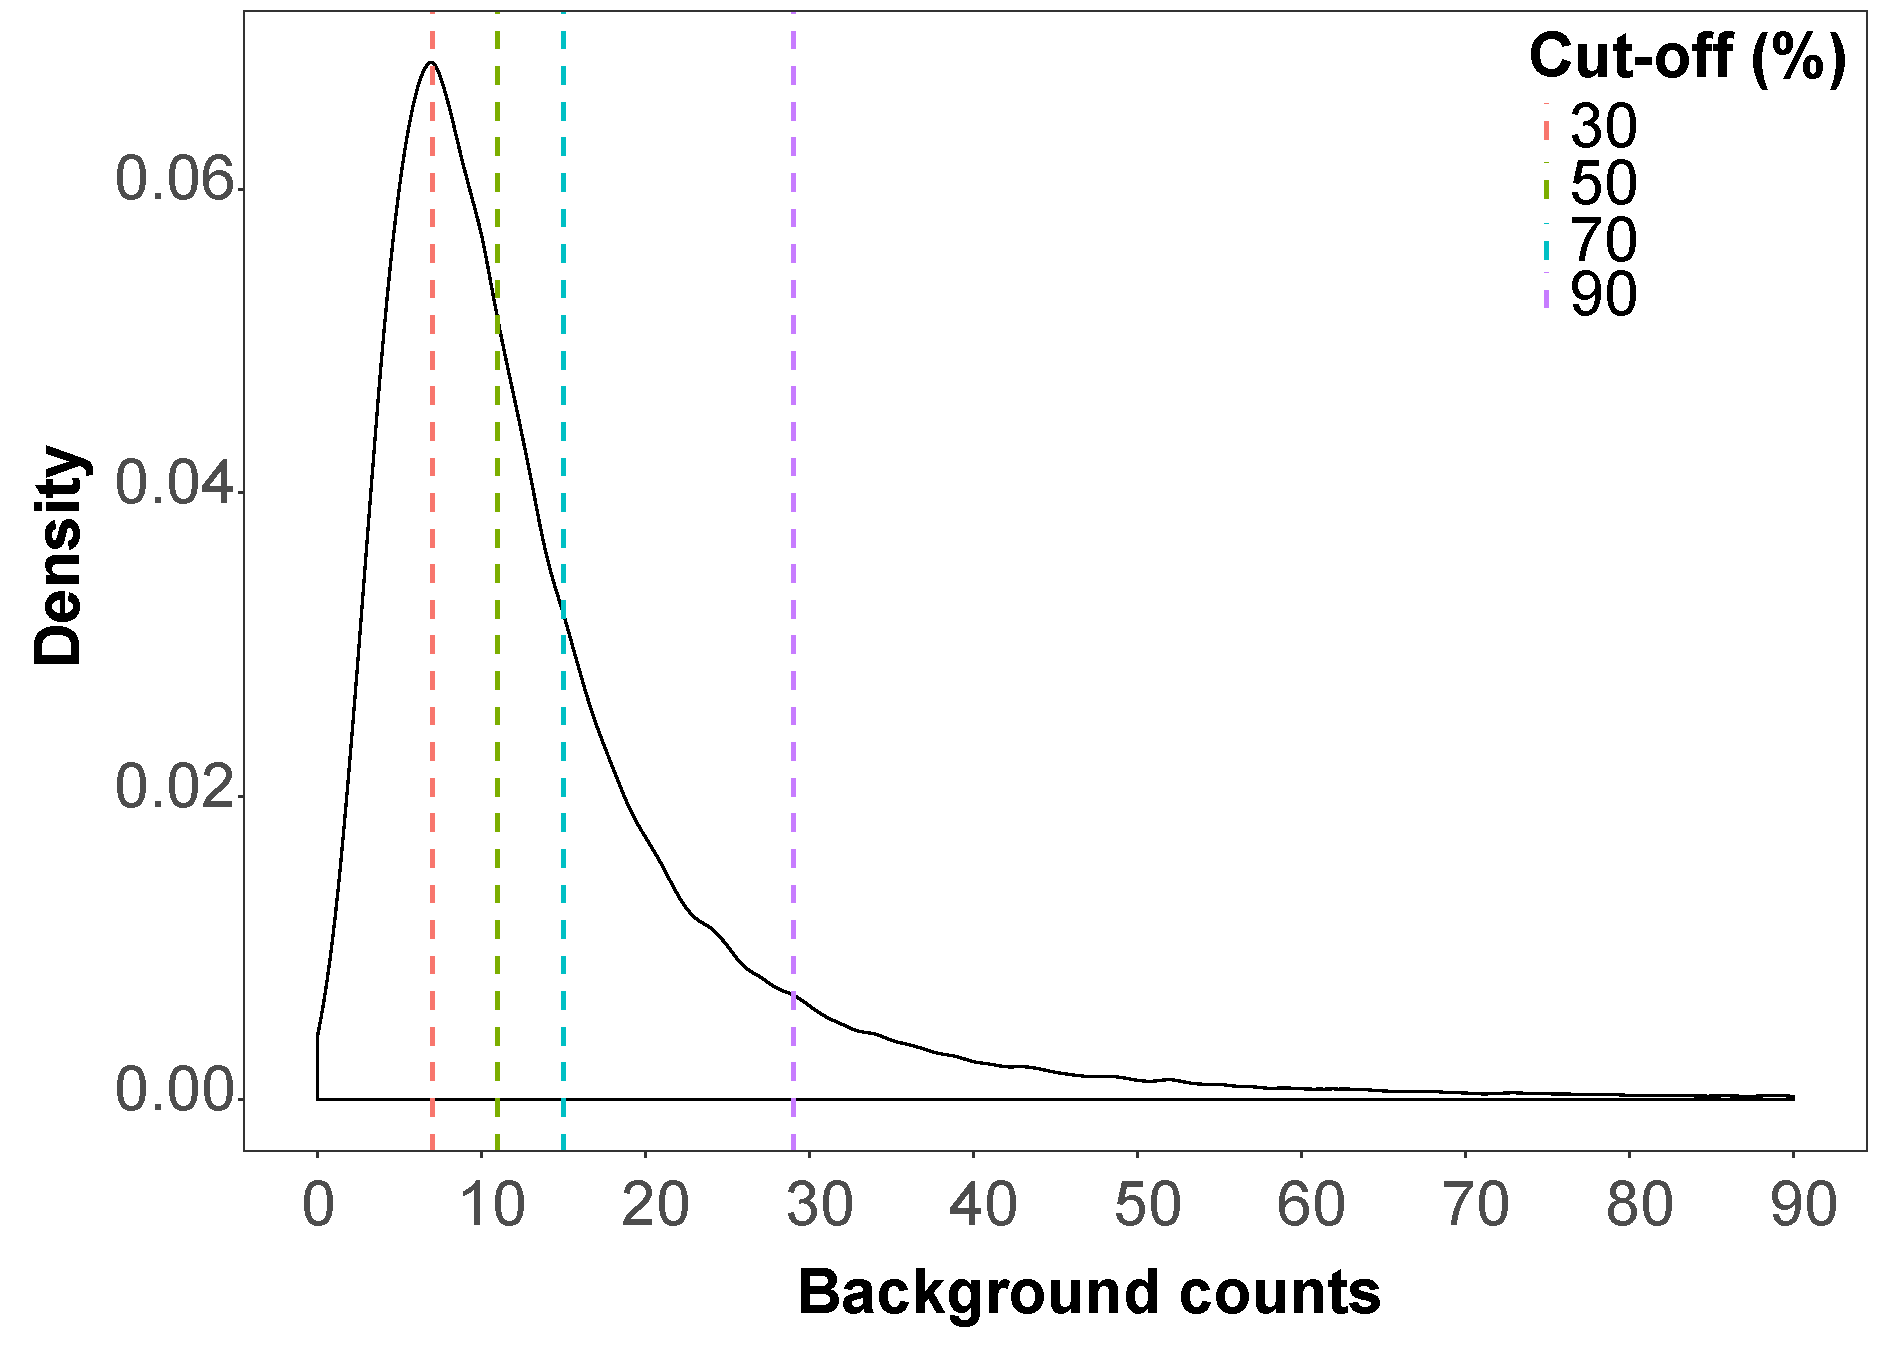
\includegraphics[width=0.5\textwidth]{./Appendix/pdfs/Chapter3/ATAC_absent_peaks_noise_distribution}
\caption[Distribution of the background read counts from all the master list peaks absent in each sample.]{\textbf{Distribution of the background read counts from all the master list peaks absent peaks in each sample.} Each cut-off corresponds to the number of background counts showed by a particular percentage of the total number of absent peaks.}
\label{figure:ATAC_absent_peaks_distribution}
\end{figure}



\begin{figure}[htbp]
\centering
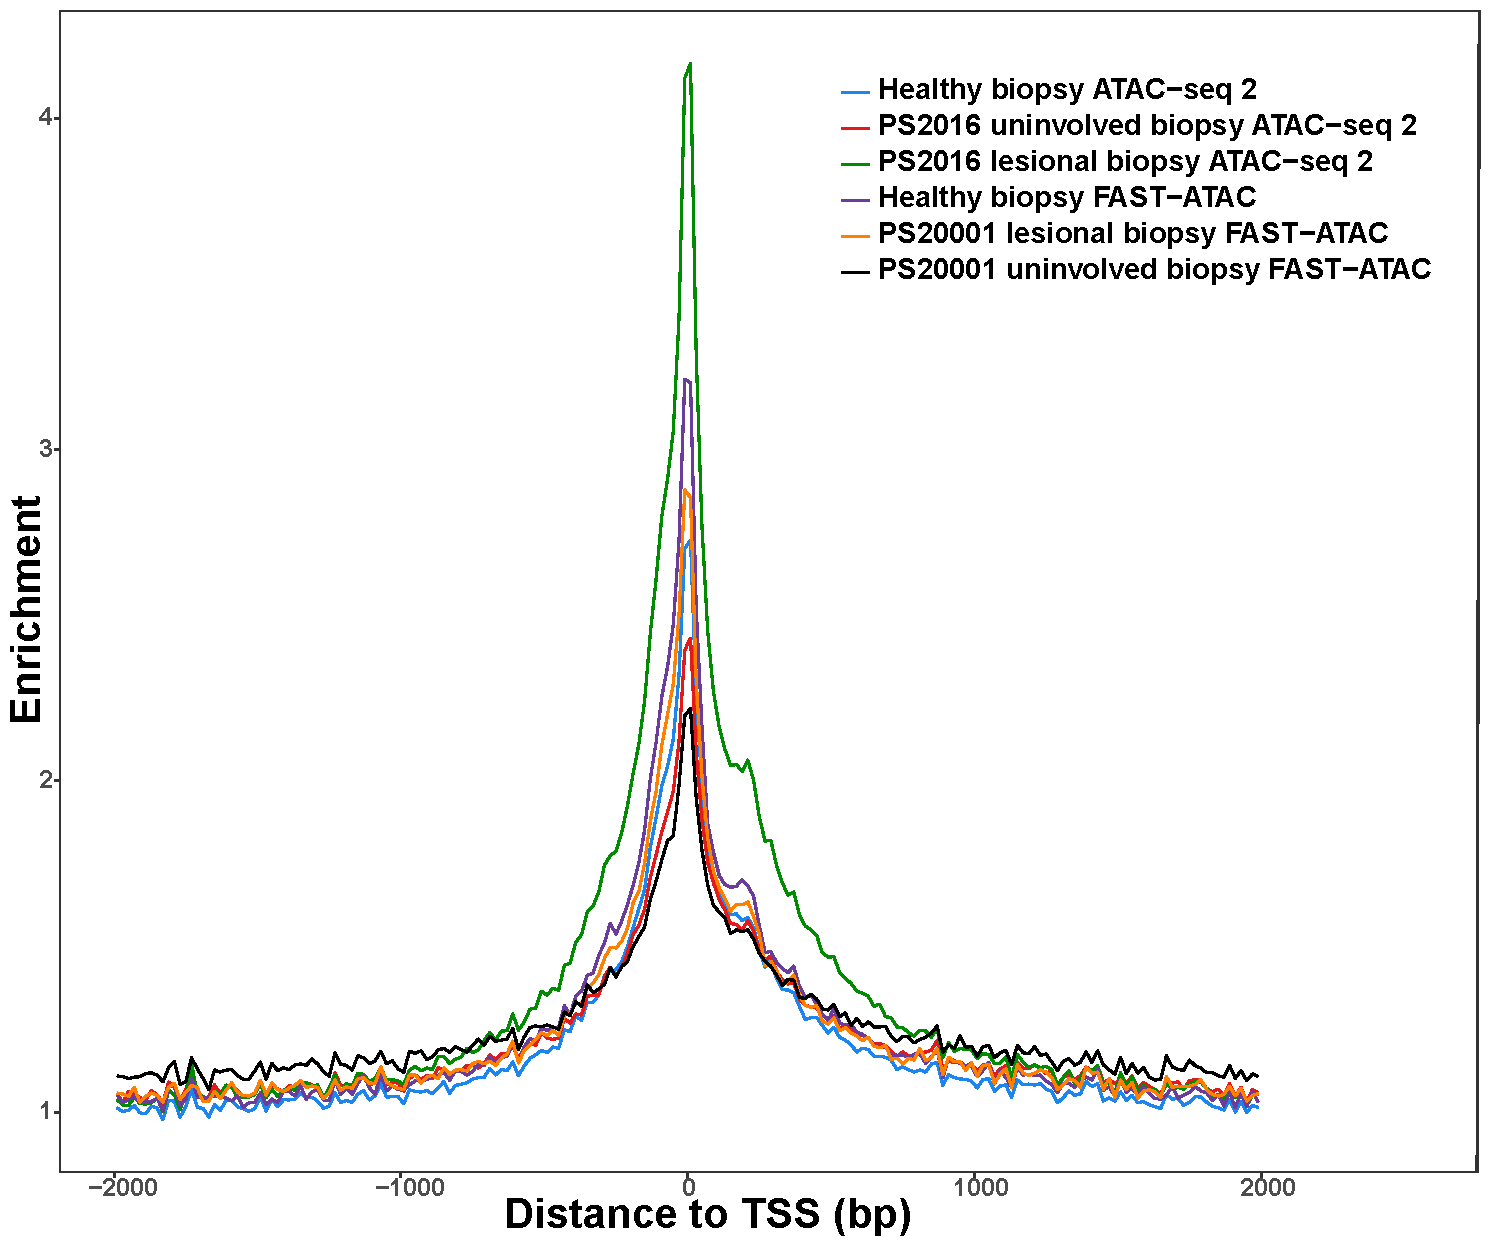
\includegraphics[width=0.5\textwidth]{./Appendix/pdfs/Chapter3/ATAC_skin_biopsy_samples_all_methods_TSS_enrichment_supplementary}
\caption[Assessment of TSS enrichment from ATAC 1 and Fast-ATAC in healthy and psoriasis KCs isolated from skin biopsy samples.]{\textbf{Assessment of TSS enrichment from ATAC 1 and Fast-ATAC in healthy and psoriasis KCs isolated from skin biopsy samples.} Fold-enrichment of ATAC fragments across the Ensembl annotated TSS from the different ATAC libraries.}
\label{figure:TSS_skin_biopsies}
\end{figure}



\begin{figure}[htbp]
\centering
\begin{subfigure}{0.70\textwidth}
\centering
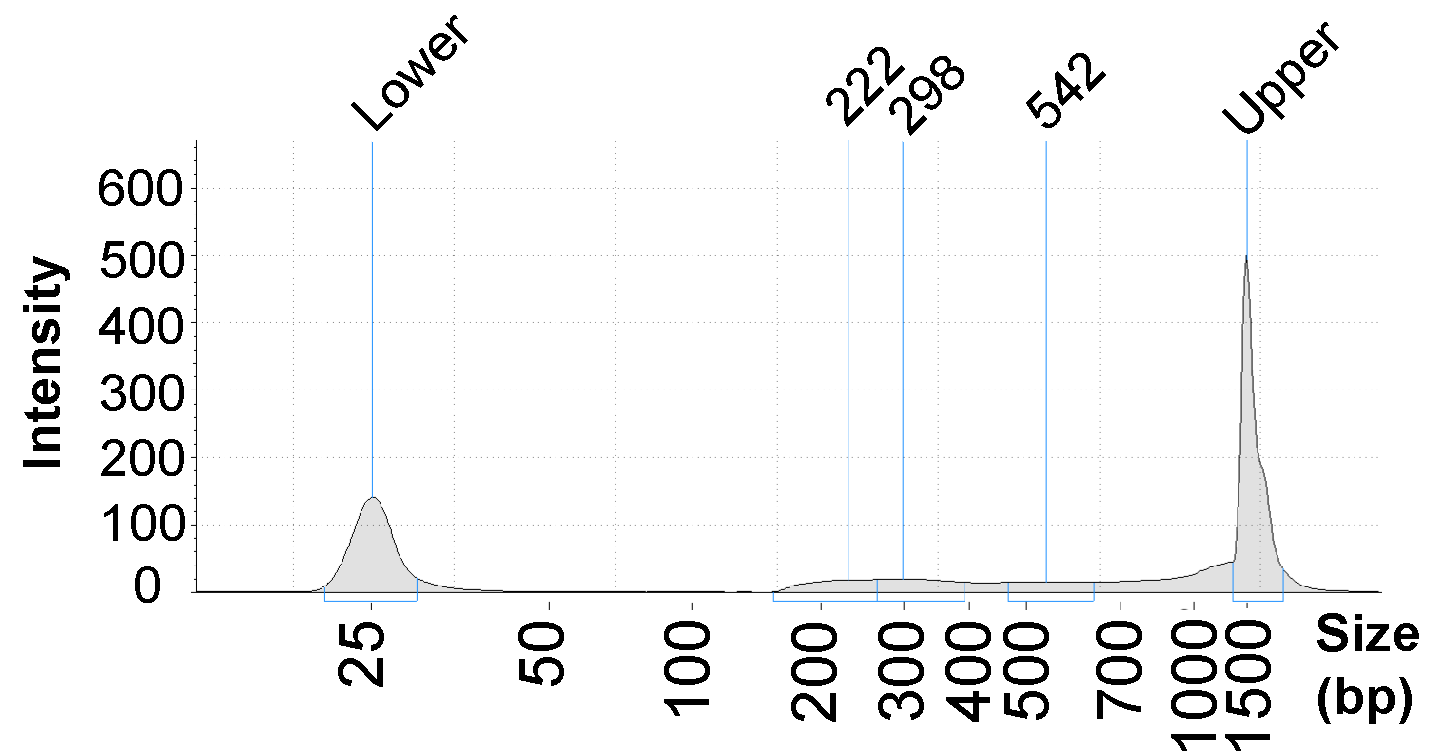
\includegraphics[width=\textwidth]{./Appendix/pdfs/Chapter3/FAST_ATAC_skin_tapestation_C1}
\caption{\textbf{}}
% The percentage sign indicated that the other subfig goes side by side
\end{subfigure}
\begin{subfigure}{0.60\textwidth}
\centering
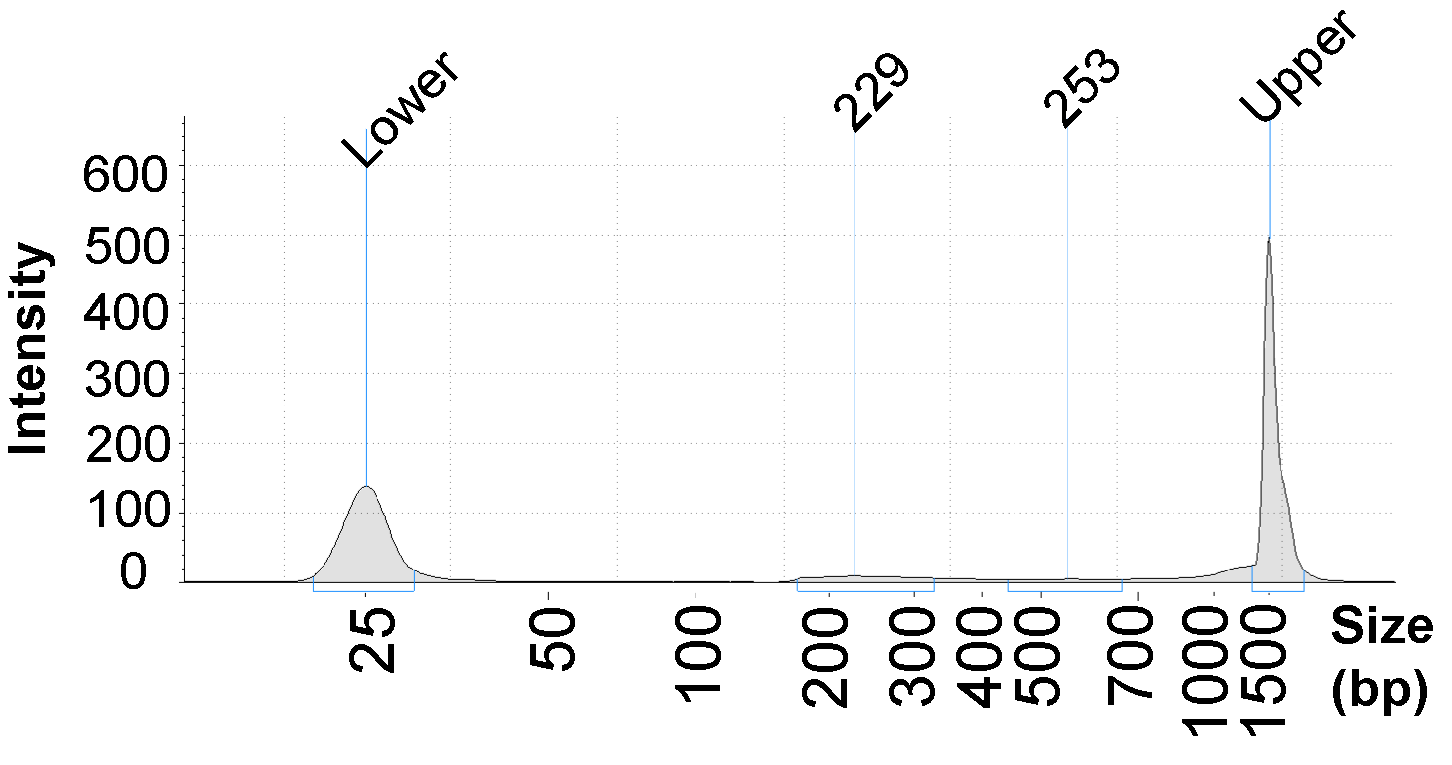
\includegraphics[width=\textwidth]{./Appendix/pdfs/Chapter3/FAST_ATAC_skin_tapestation_C3}
\caption{\textbf{}}
\end{subfigure}
\begin{subfigure}{0.60\textwidth}
\centering
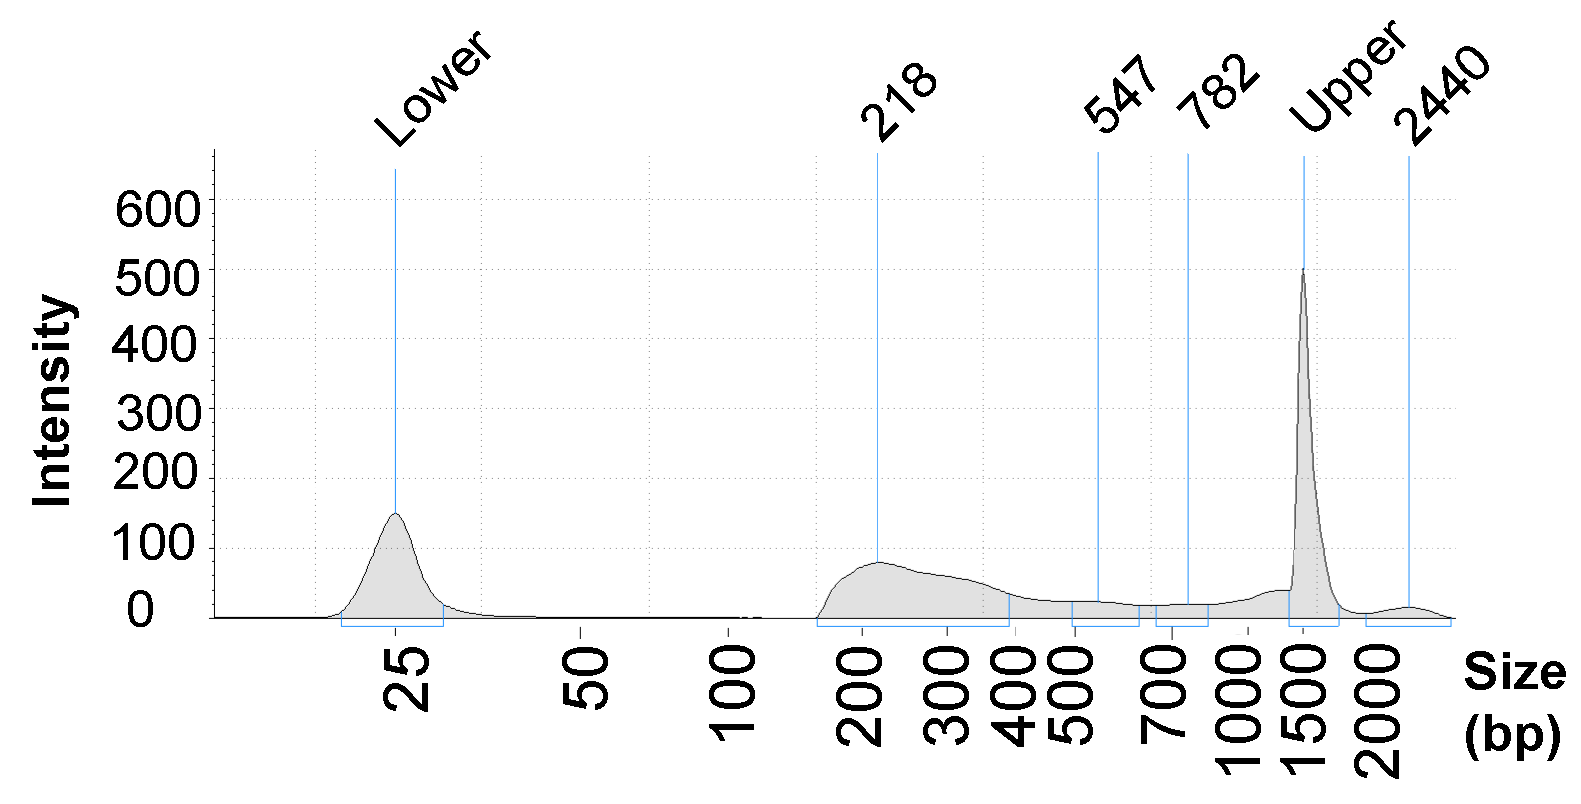
\includegraphics[width=\textwidth]{./Appendix/pdfs/Chapter3/FAST_ATAC_skin_tapestation_C4}
\caption{\textbf{}} % to add text to the figure name
\end{subfigure}
\begin{subfigure}{0.60\textwidth}
\centering
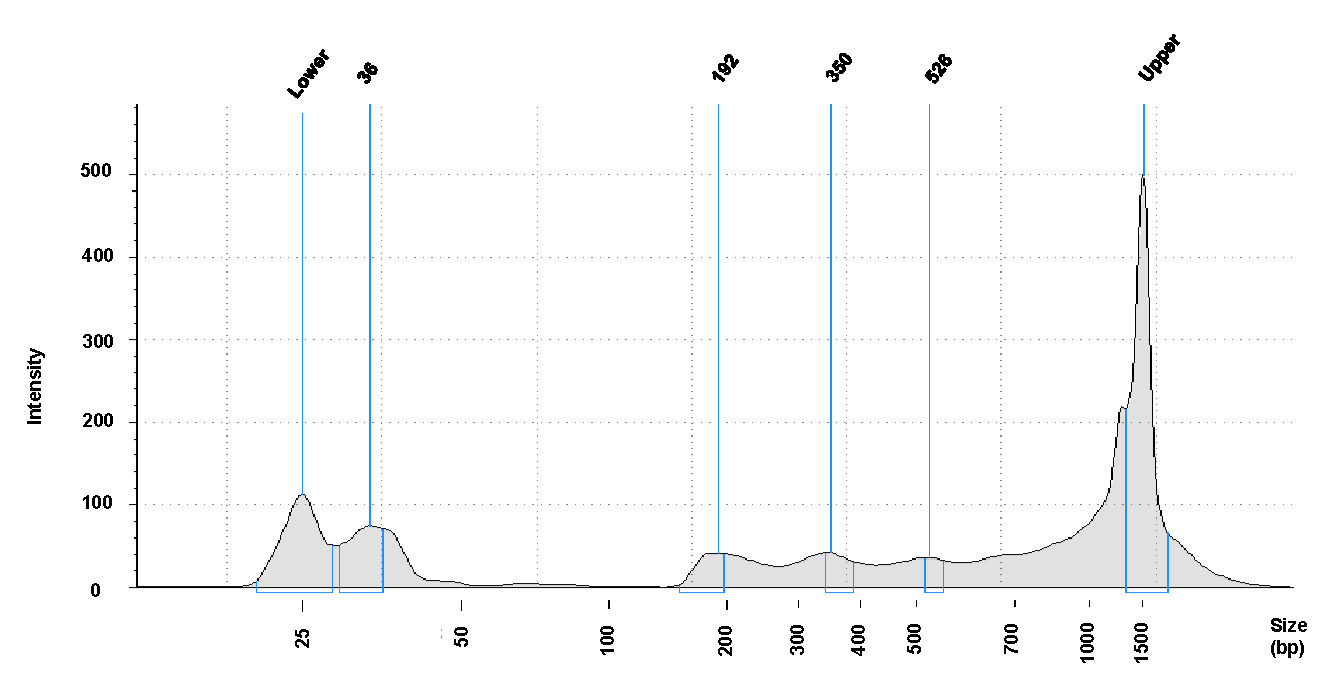
\includegraphics[width=\textwidth]{./Appendix/pdfs/Chapter3/Omni_ATAC_NHEK_Rep1_tapestation}
\caption{\textbf{}} % to add text to the figure name
\end{subfigure}
\hfill
\caption[Fast-ATAC and Omni-ATAC NHEK tapestation profiles.]{\textbf{Fast-ATAC and Omni-ATAC NHEK tapestation profiles.} Pre-sequencing quantification of DNA fragment sizes from the libraries generated  using the a) C2, b) C3, and c) C4 versions of the Fast-ATAC protocol based on modifications in the detergent and Tn5 concentration and d) Omni-ATAC. C2, C3 and C4 detergent and Tn5 concentrations are detailed in Table \ref{tab:ATAC_skin_optimisation_protocols}.}
\label{figure:NHEK_tapestation}
\end{figure}

\section{Chapter 4 Figures}

\begin{figure}[htbp]
\centering
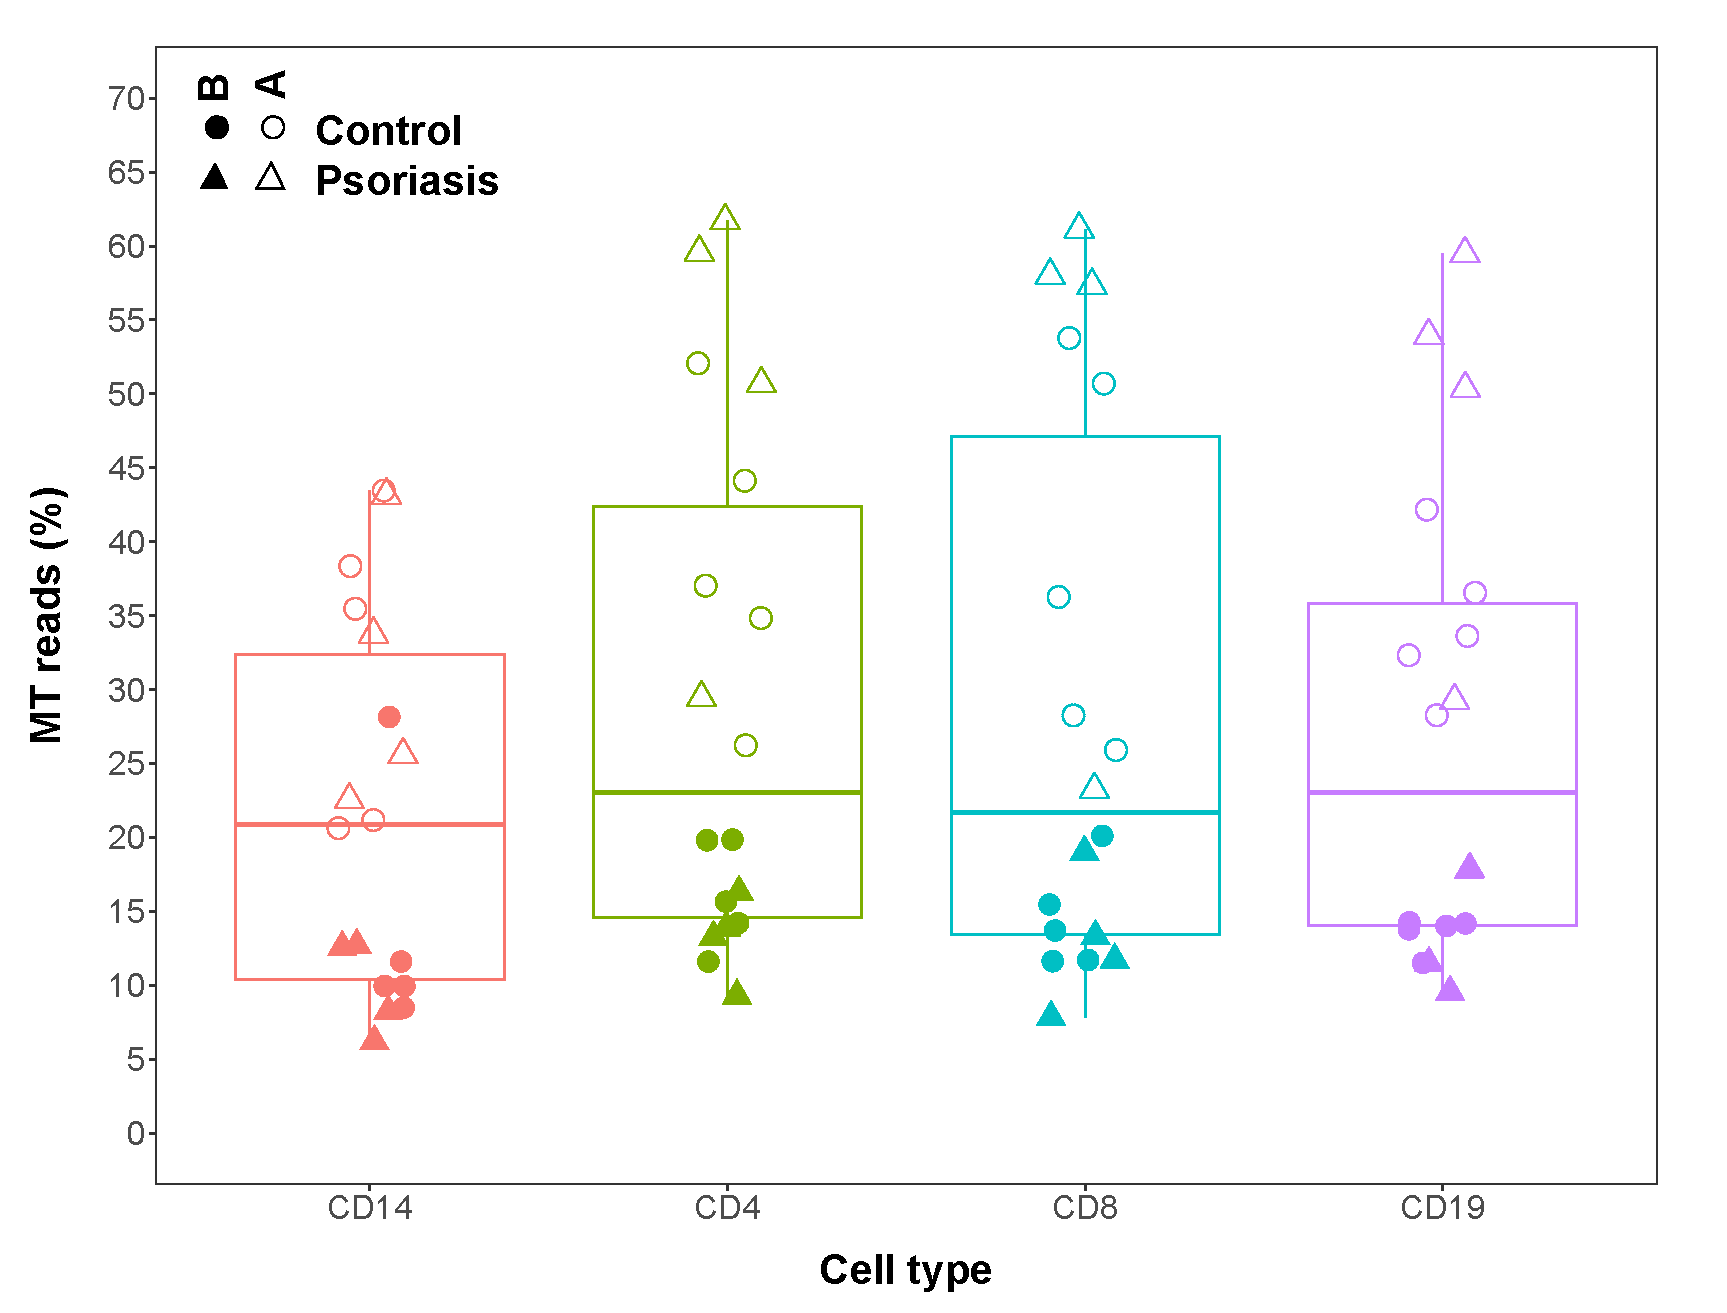
\includegraphics[width=0.6\textwidth]{./Appendix/pdfs/Chapter4/ATAC_PS_CTL_MT_percent_boxplot}
\caption[Percentage of MT reads in the ATAC-seq libraries generated in CD14$^+$ monocytes, CD4$^+$, CD8$^+$ and CD19$^+$ isolated from psoriasis patients and healthy controls.]{\textbf{Percentage of MT reads in the ATAC-seq samples generated in CD14$^+$ monocytes, CD4$^+$, CD8$^+$ and CD19$^+$ isolated from psoriasis patients and healthy controls.} Samples from cohort 1A (open circlues and triangles) were generated with the standard ATAC-seq protocol from Buenrostro \textit{et al.}, 2013 whereas samples from cohort 1B (filles circles and triangles) were processed using FAST-ATAC \parencite{Corces2016}.}
\label{fig:ATAC_PS_CTL_MT_percent}
\end{figure}


\begin{figure}[htbp]
\centering
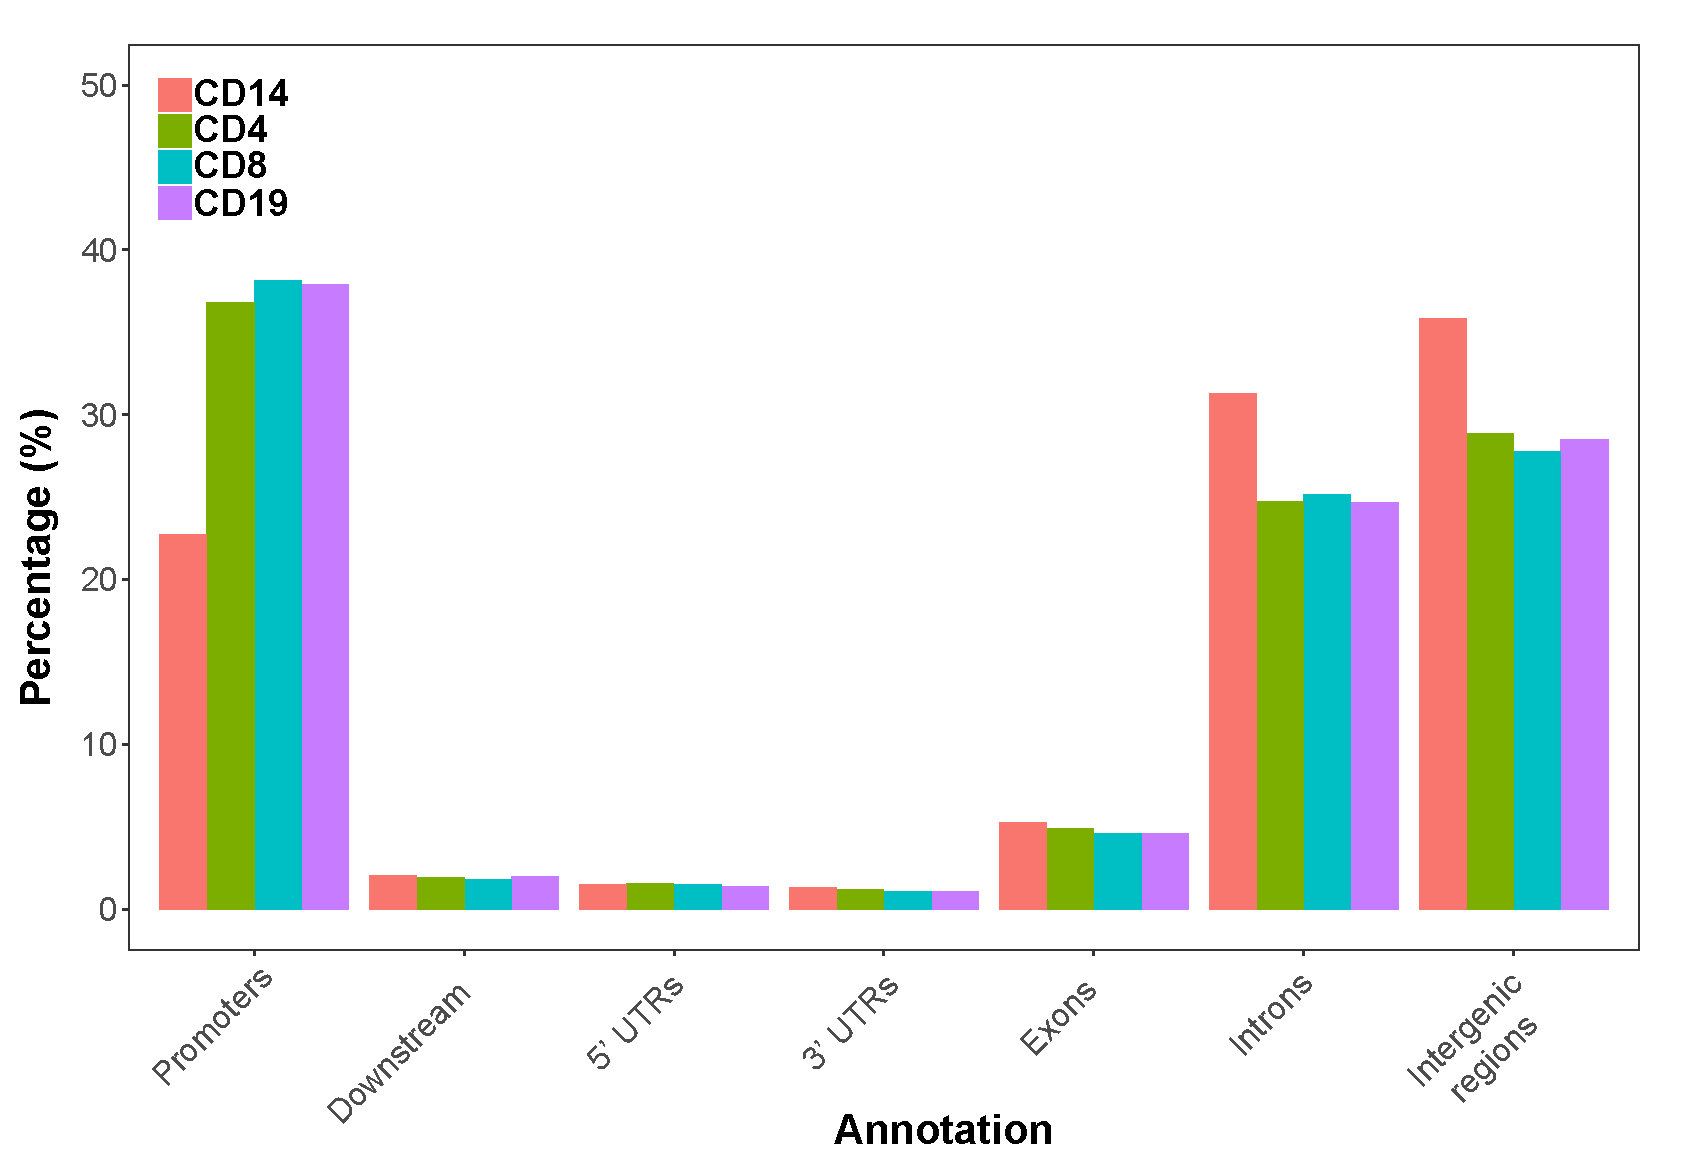
\includegraphics[width=0.6\textwidth]{./Appendix/pdfs/Chapter4/ATAC_all_cell_types_individual_master_lists_general_peak_annotation}
\caption[Genomic annotation of the consensus master list of ATAC-seq enriched sites built for downstream differential chromatin accessibility analysis in CD14$^+$ monocytes, CD4$^+$, CD8$^+$ and CD19$^+$.]{\textbf{Genomic annotation of the consensus master list of ATAC-seq enriched sites built for downstream differential chromatin accessibility analysis in CD14$^+$ monocytes, CD4$^+$, CD8$^+$ and CD19$^+$.} Annotation is expressed in percentage over the total number of ATAC-seq sites included in each particular cell type master list.}
\label{fig:ATAC_PS_CTL_genomic_annotation}
\end{figure}


\bigskip
\begin{figure}[htbp]
\centering
\begin{subfigure}[b]{0.50\textwidth}
\centering 
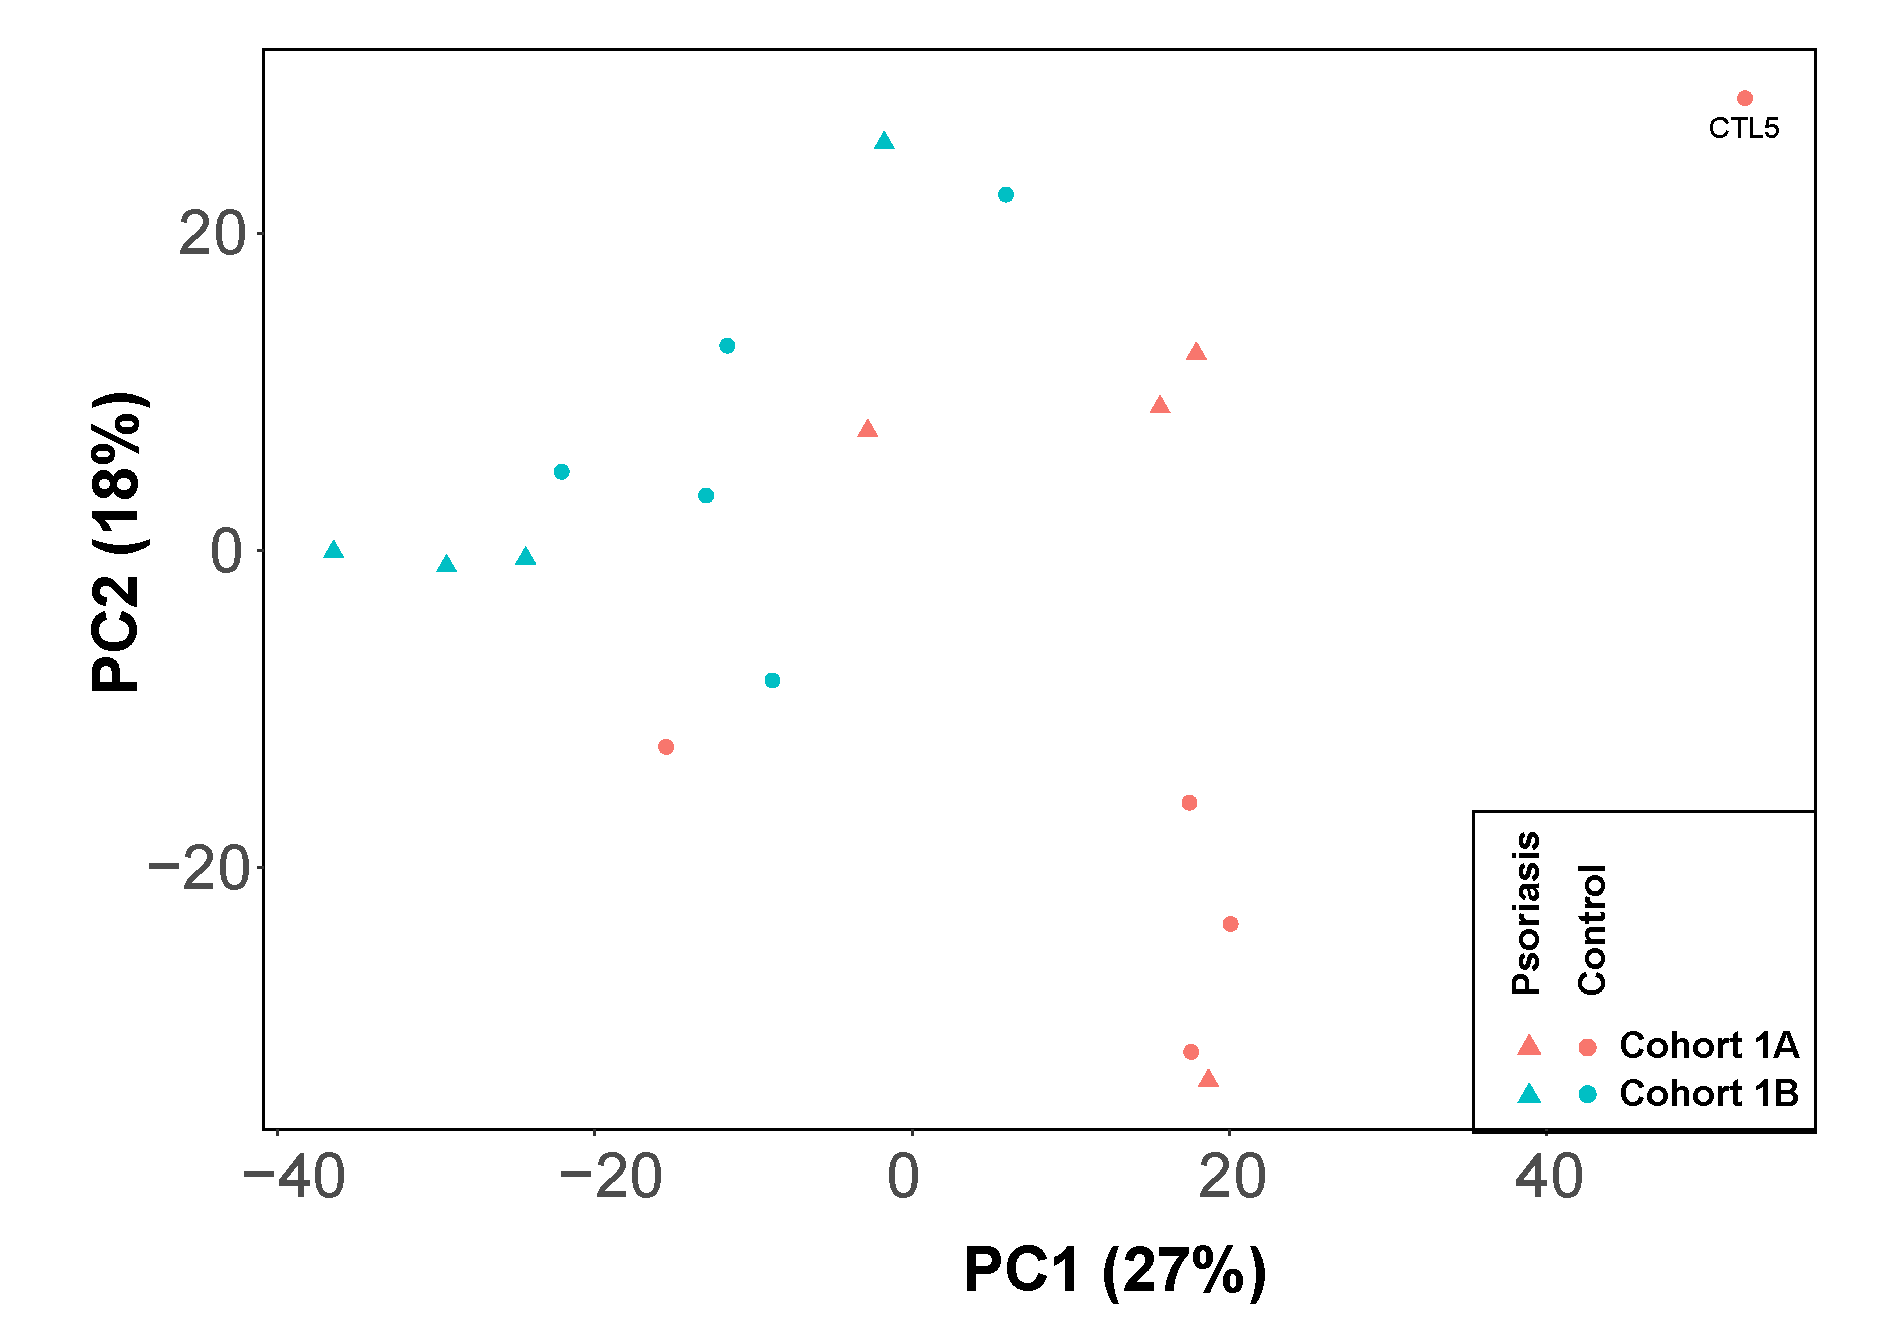
\includegraphics[width=\textwidth]{./Appendix/pdfs/Chapter4/ATAC_CD8_PS_CTL_PCA}
\caption{}
\end{subfigure}
~
\begin{subfigure}[b]{0.50\textwidth} 
%the [b] prevents offset in subcaptions
\centering
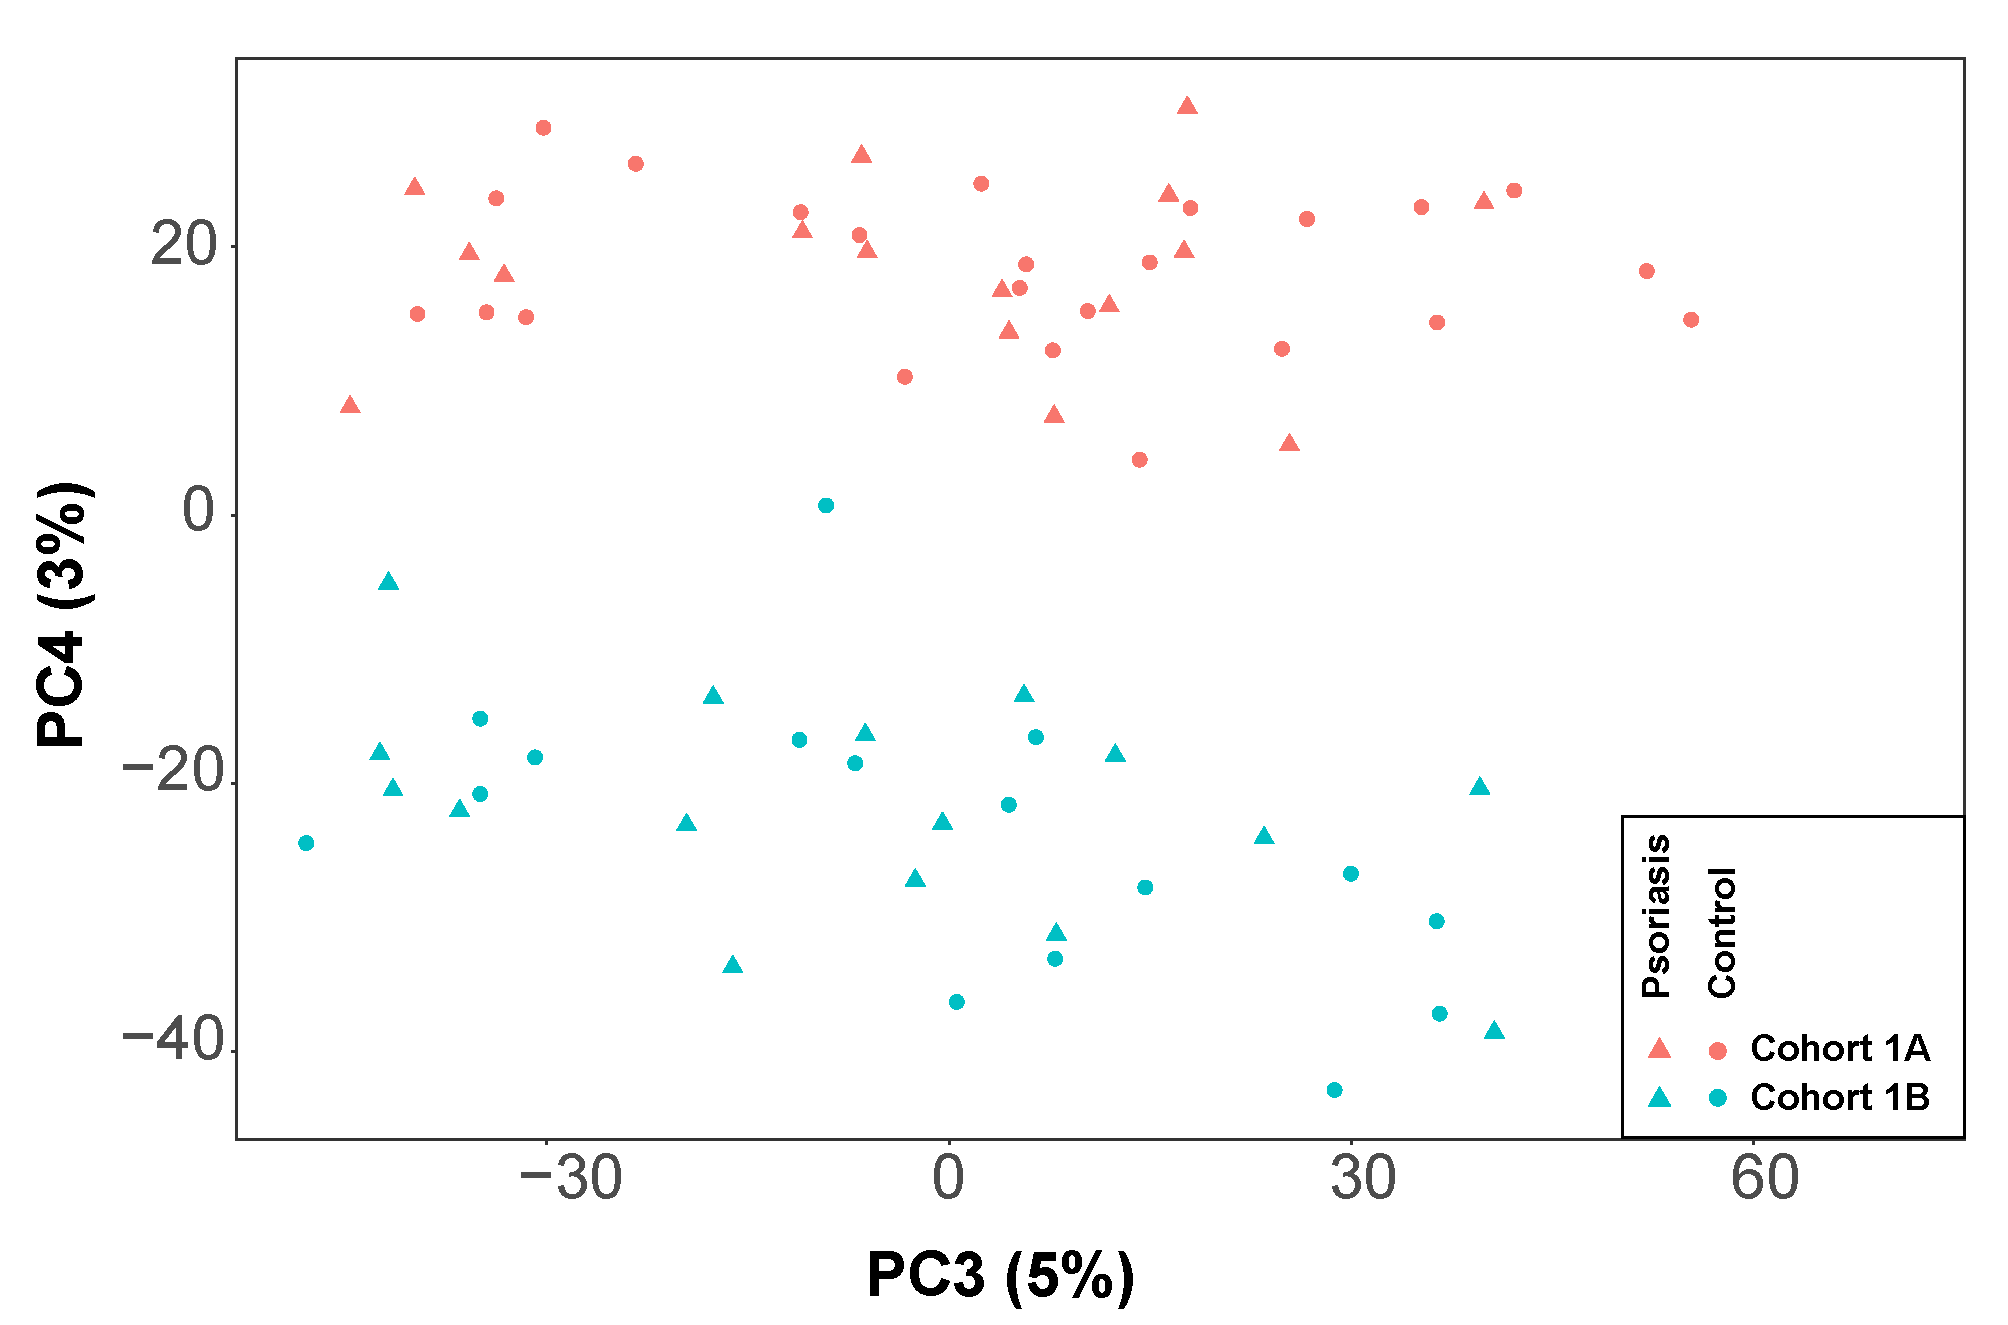
\includegraphics[width=\textwidth]{./Appendix/pdfs/Chapter4/PS_CTL_all_samples_varied_PCA3and4_plot}
\caption{}
\end{subfigure}
\caption[PCA analysis illustrating batch effect in ATAC-seq and RNA-seq samples.]{\textbf{PCA analysis illustrating batch effect in ATAC-seq and RNA-seq samples.} a) xxxx  b)}
\label{figure:ATAC_RNAseq_batch_effect}
\end{figure}



\section{Chapter 5 Figures}

\bigskip
\begin{figure}[htbp]
\centering
\begin{subfigure}[b]{0.45\textwidth}
\centering 
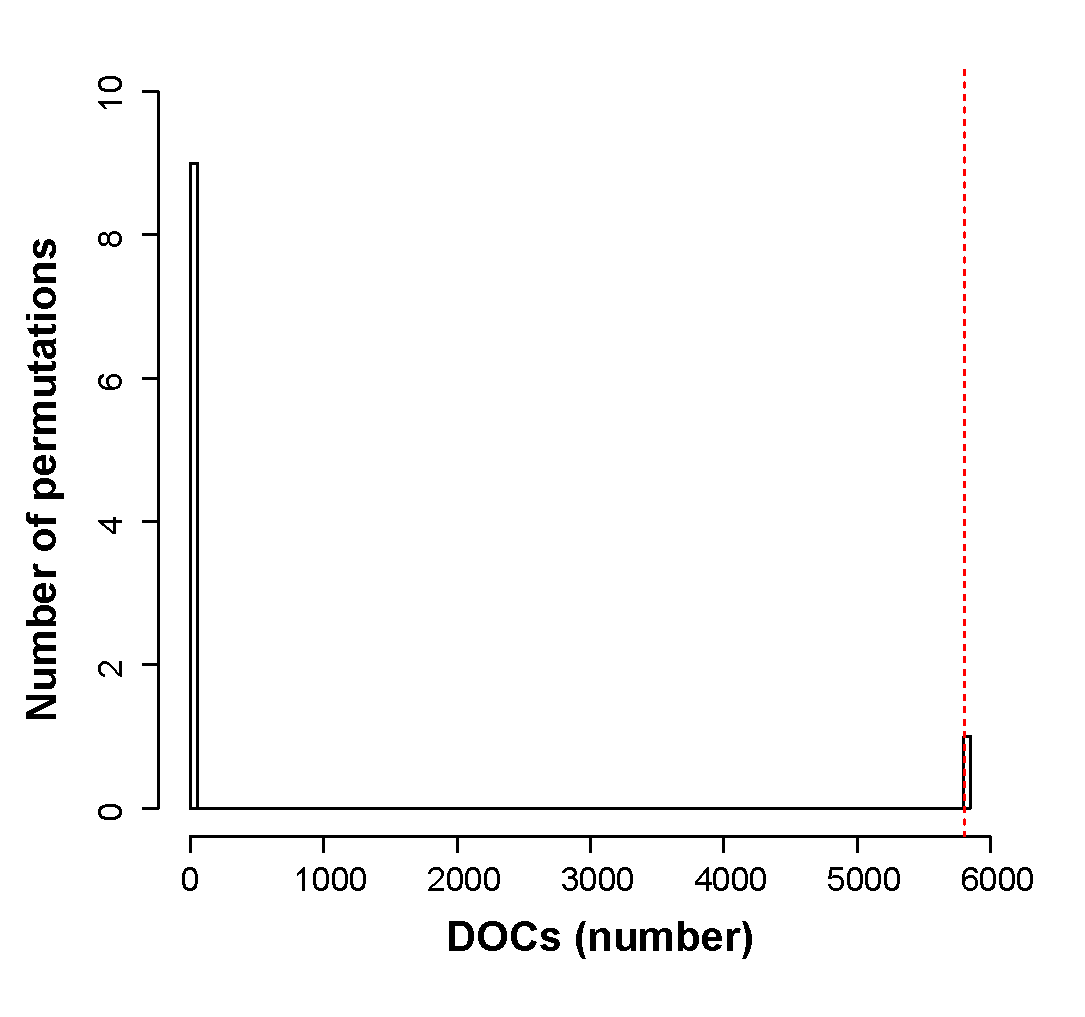
\includegraphics[width=\textwidth]{./Appendix/pdfs/Chapter5/ATAC_PsA_CD14_permutation_analysis}
\caption{}
\end{subfigure}
~
\begin{subfigure}[b]{0.45\textwidth}
\centering 
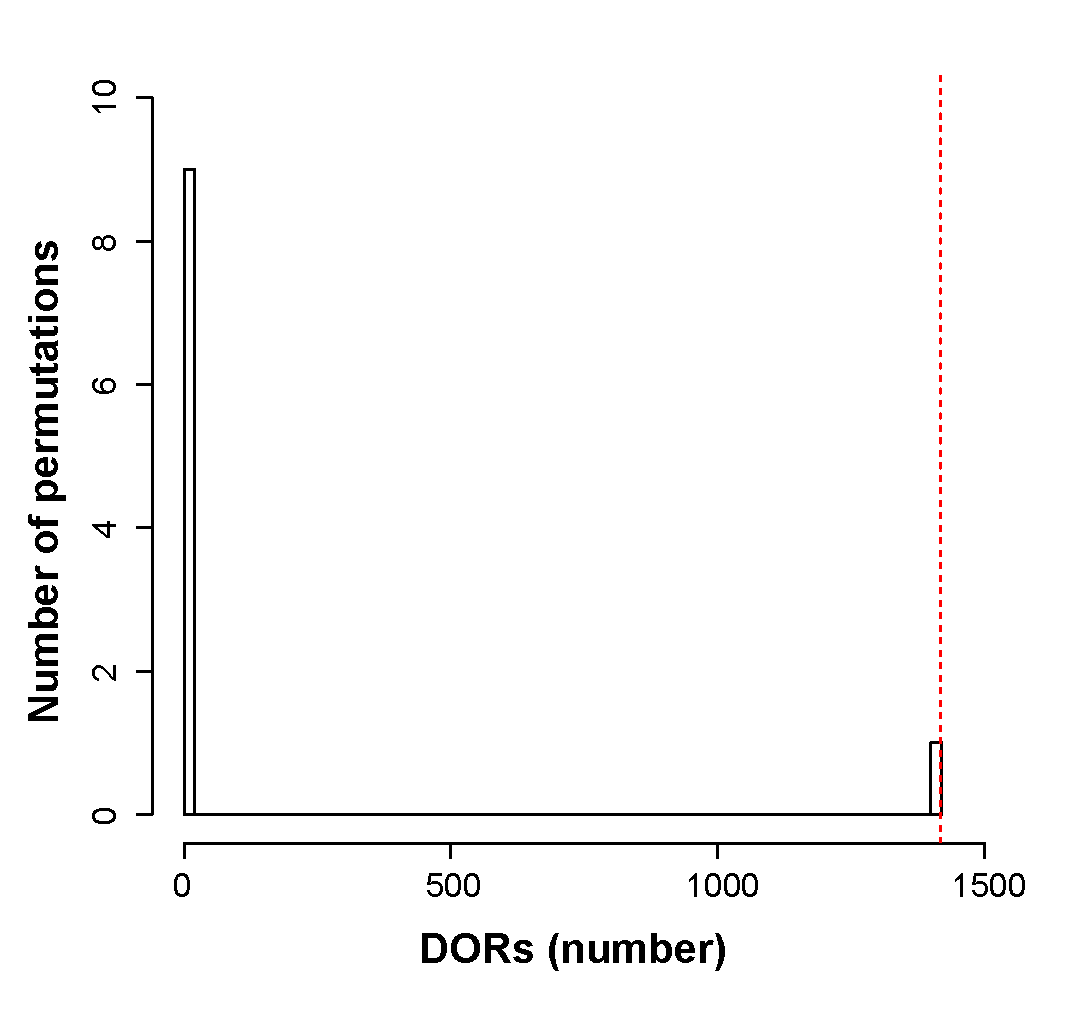
\includegraphics[width=\textwidth]{./Appendix/pdfs/Chapter5/ATAC_PsA_CD4_permutation_analysis}
\caption{}
\end{subfigure}
~
\begin{subfigure}[b]{0.45\textwidth} 
%the [b] prevents offset in subcaptions
\centering
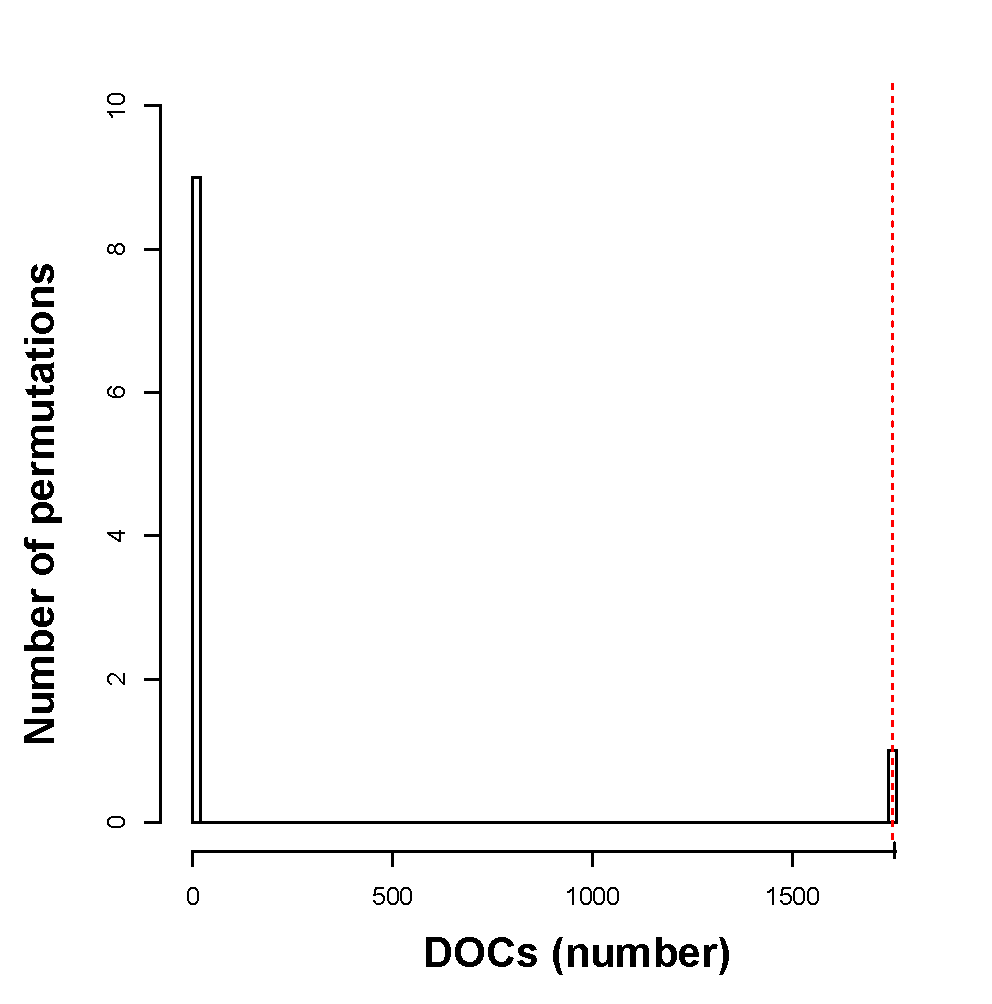
\includegraphics[width=\textwidth]{./Appendix/pdfs/Chapter5/ATAC_PsA_CD8_permutation_analysis}%
\caption{}
\end{subfigure}
\begin{subfigure}[b]{0.45\textwidth} 
%the [b] prevents offset in subcaptions
\centering
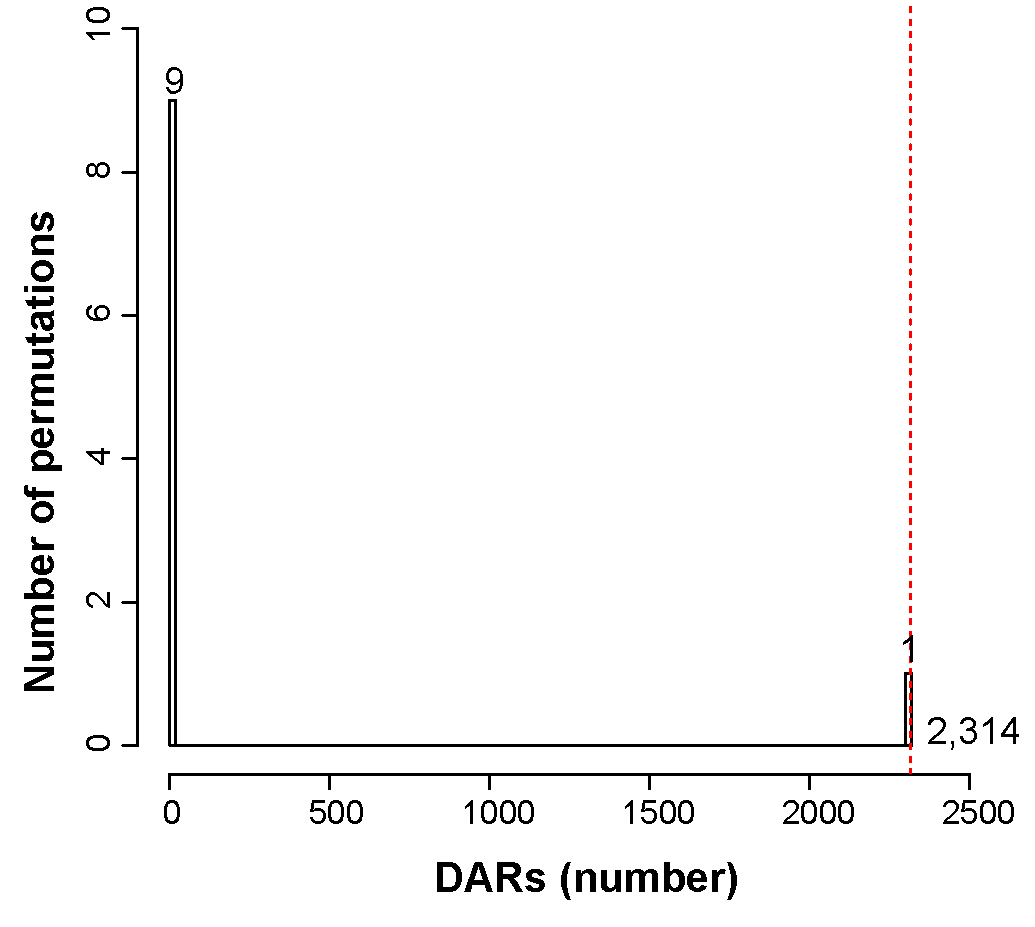
\includegraphics[width=\textwidth]{./Appendix/pdfs/Chapter5/ATAC_PsA_NK_permutation_analysis}%
\caption{}
\end{subfigure}
\caption[Permutation analysis SF vs PB in CD14$^+$,CD4m$^+$,CD8m$^+$ and NK.]{\textbf{Permutation analysis SF vs PB in CD14$^+$,CD4m$^+$,CD8m$^+$ and NK.} Sample labels were permuted within each cell type to achieve the ten unique possible combinations and differential analysis was performed. The number of significant DARs (FDR$<$0.01 and no abs(FC)$>$1.5) across all permutations in plotted for a)  CD14$^+$, b) CD4m$^+$, c)CD8m$^+$ and d) NK, demonstrating that the true observation (dashed red line) is significantly more than expected by chance (pval$<$0.1, the lowest pval for the maximum number of permutations that can be conducted with this sample size) in all four cell types.}
\label{figure:PsA_perm_analysis}
\end{figure}



\begin{figure}[htbp]
\centering
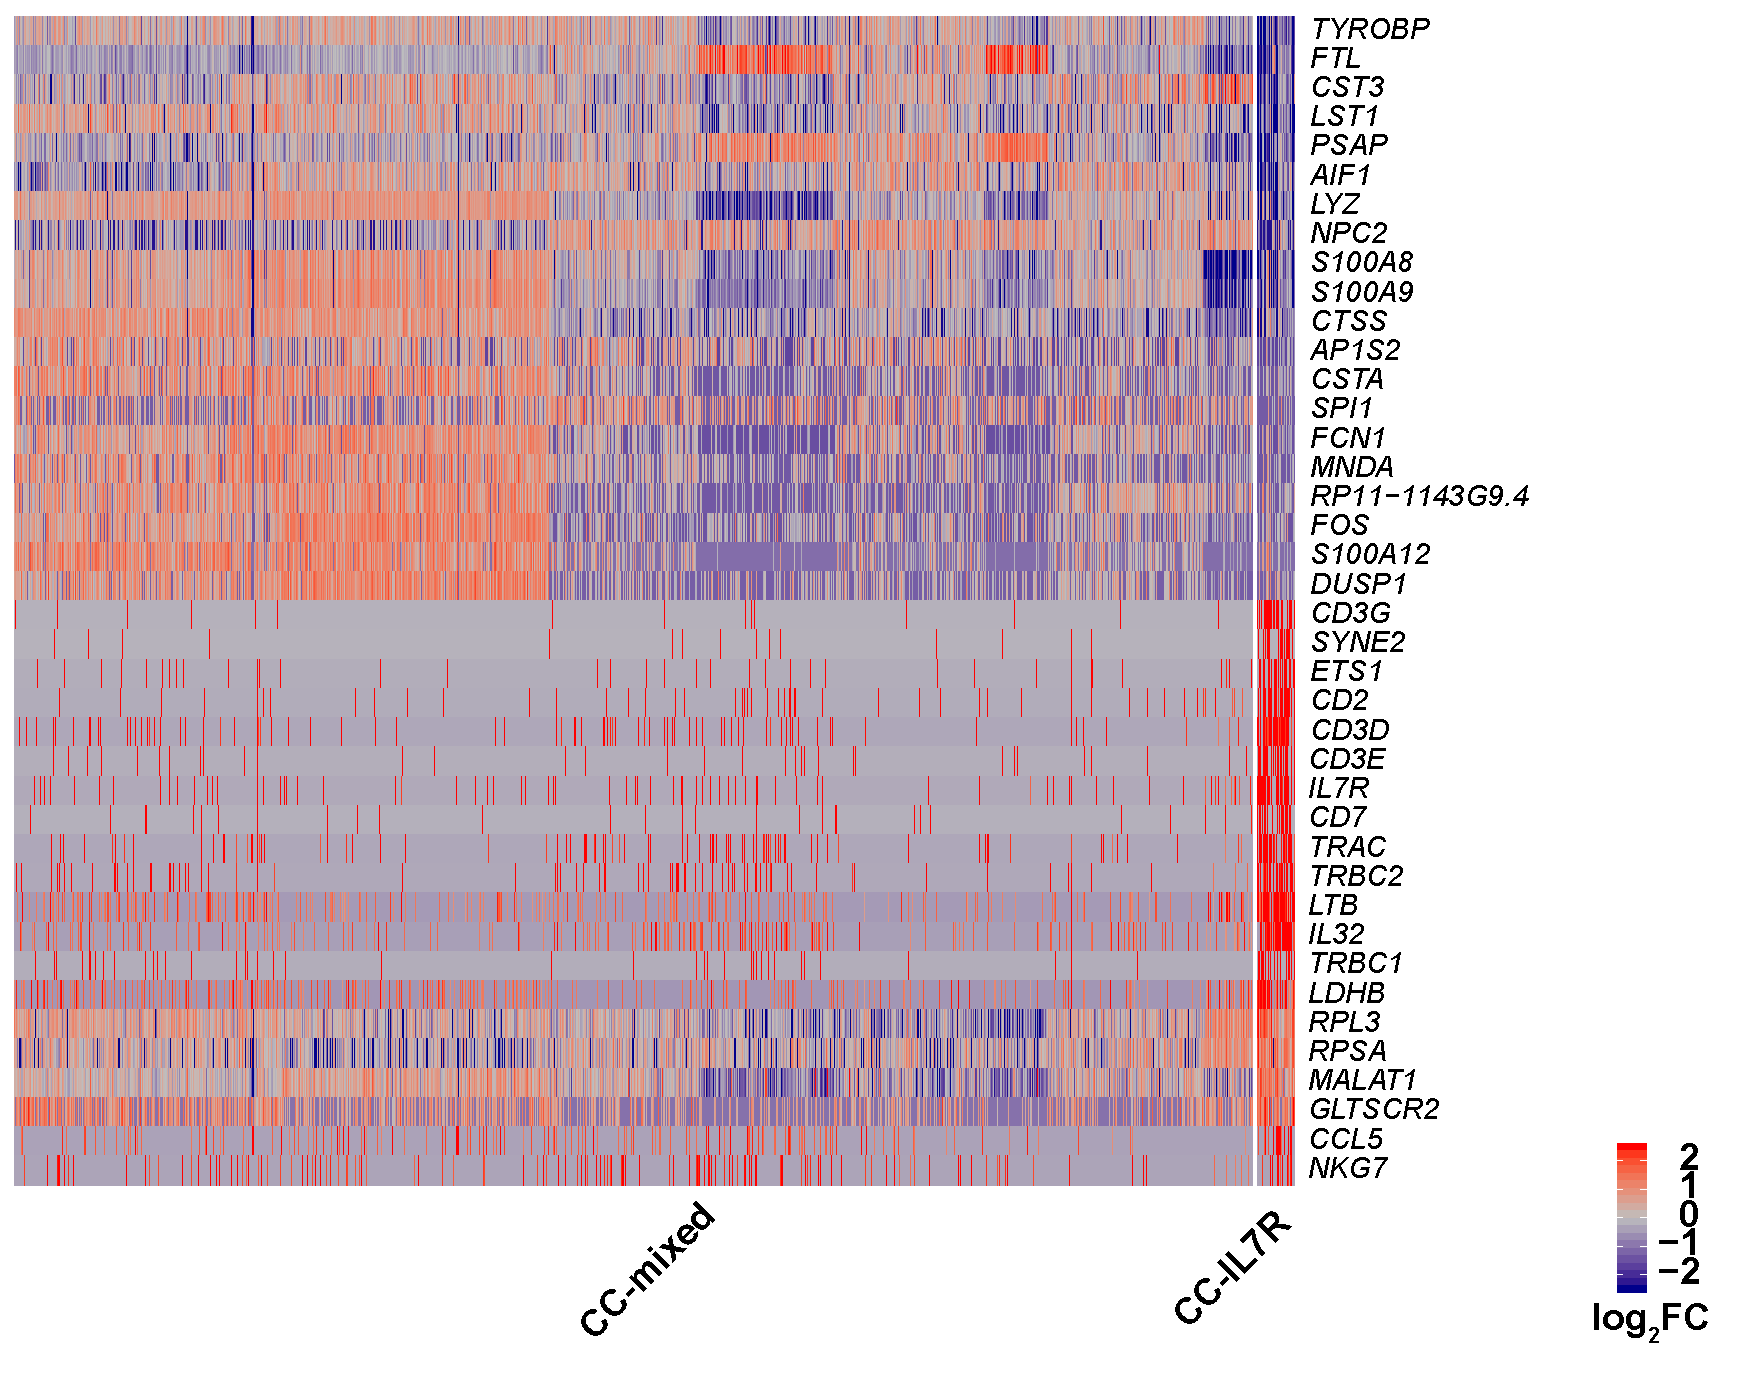
\includegraphics[width=0.6\textwidth]{./Appendix/pdfs/Chapter5/PSA_10X_heatmap_SF_PB_monocytes_clusters_mixed_and_IL7R}
\caption[Heatmap for the top 20 marker genes of the CC-mixed and CC-IL7R CD14$^+$ monocytes subpopulations.]{\textbf{Heatmap for the top 20 marker genes of the CC-mixed and CC-IL7R CD14$^+$ monocytes subpopulations.} Rows are the top 20 marker genes for each of the two subpopulations (total of 40 genes). The columns represent each of the cells members of the CC-mixed (left) or CC-IL7R (right) clusters. The colour scale represents the log$_2$FC in the expression of the marker gene in a particular cell of the cluster compared to the average expression of all the cells from the other cluster.}
\label{figure:PSA_scRNAseq_CC_mixed_and_IL7R_markers_heatmap}
\end{figure}

\bigskip
\begin{figure}[htbp]
\centering
\begin{subfigure}[b]{0.70\textwidth}
\centering 
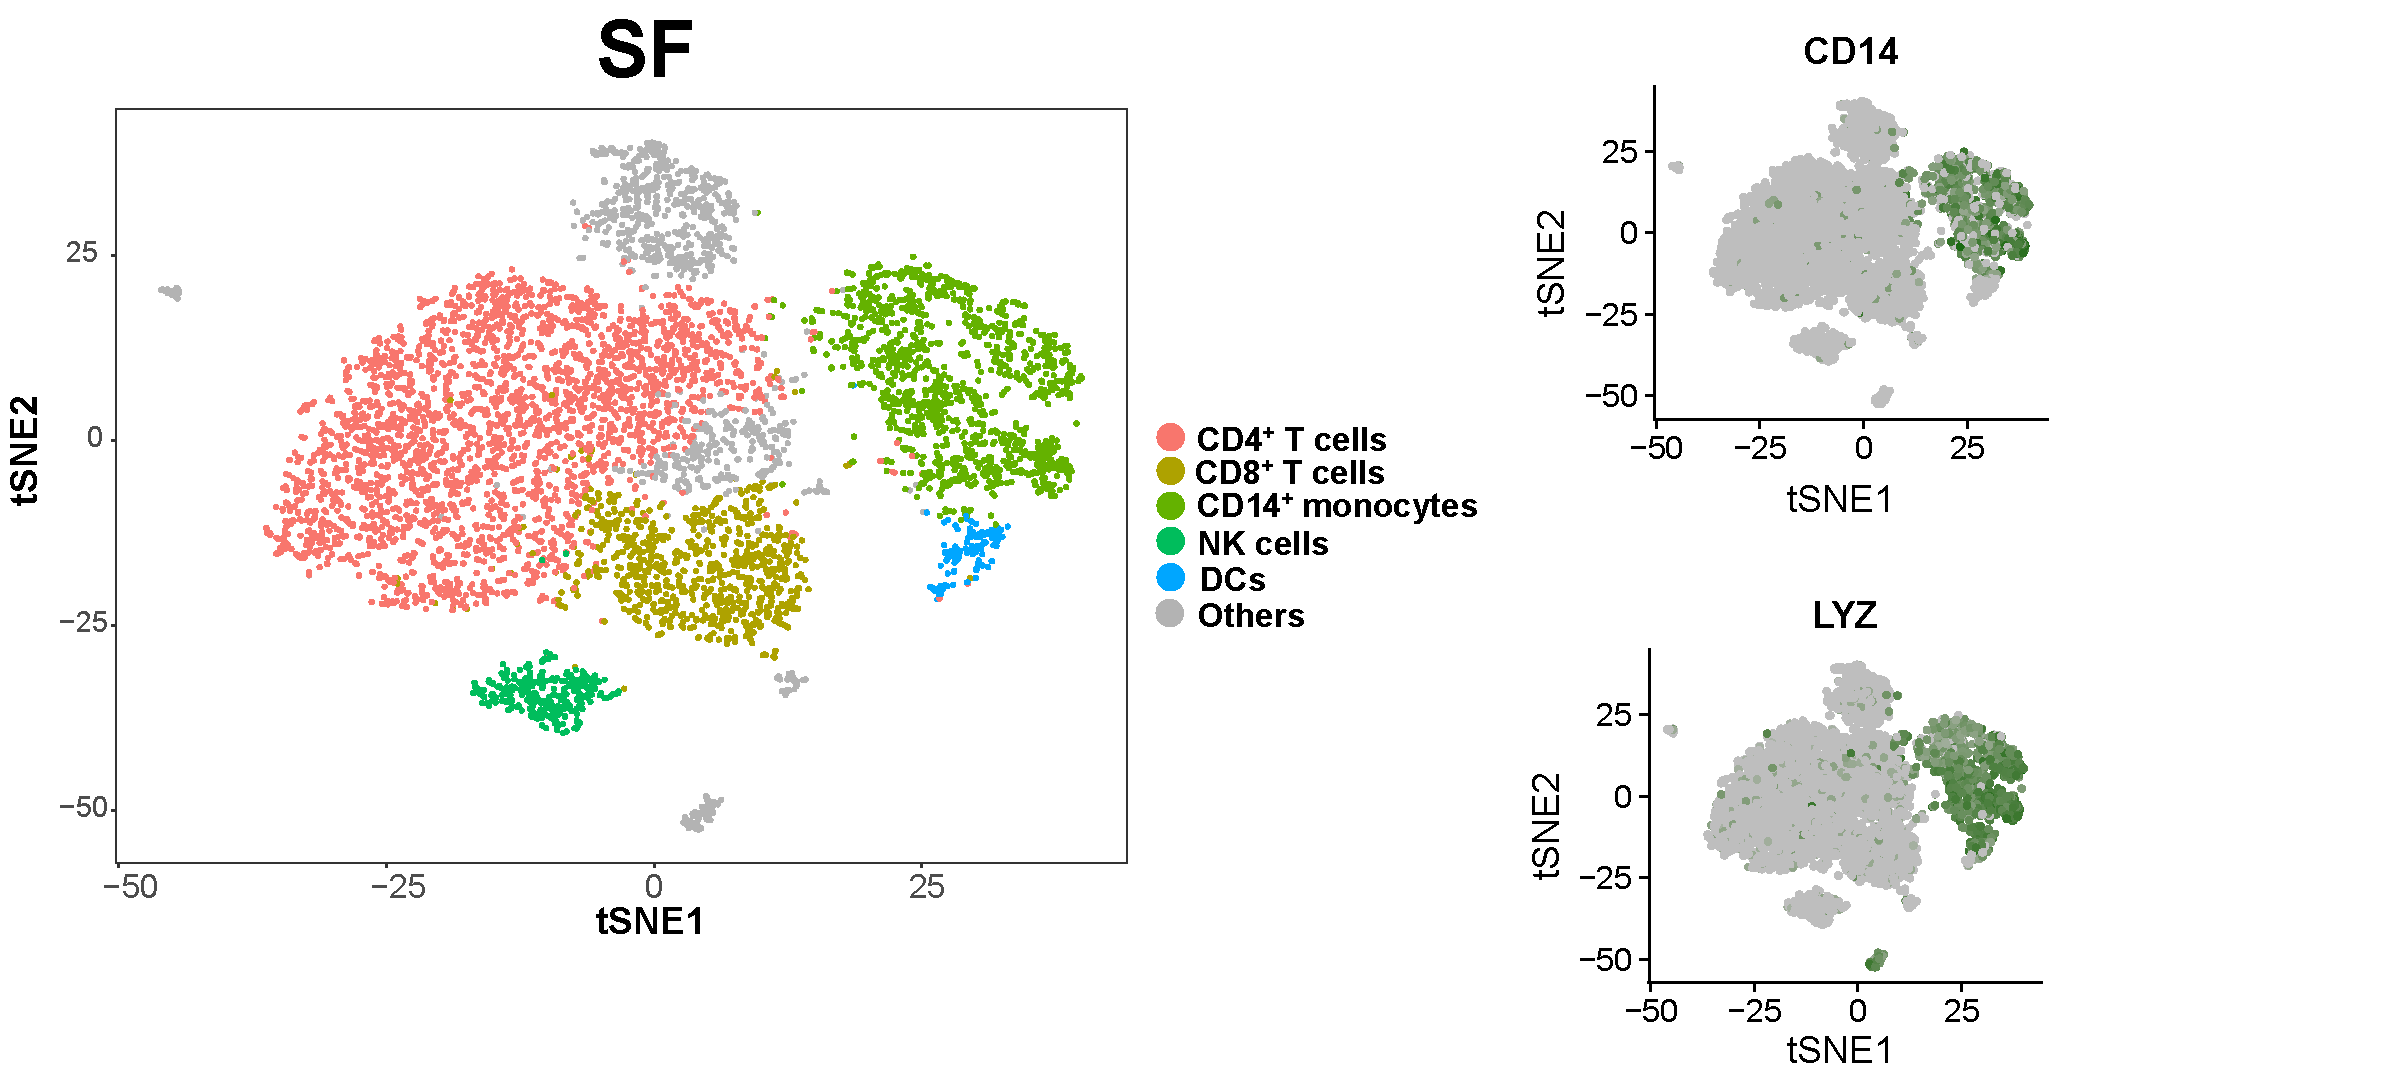
\includegraphics[width=\textwidth]{./Appendix/pdfs/Chapter5/PSA_SF_clusters_and_monocytes_markers}
\caption{}
\end{subfigure}
~
\begin{subfigure}[b]{0.70\textwidth} 
%the [b] prevents offset in subcaptions
\centering
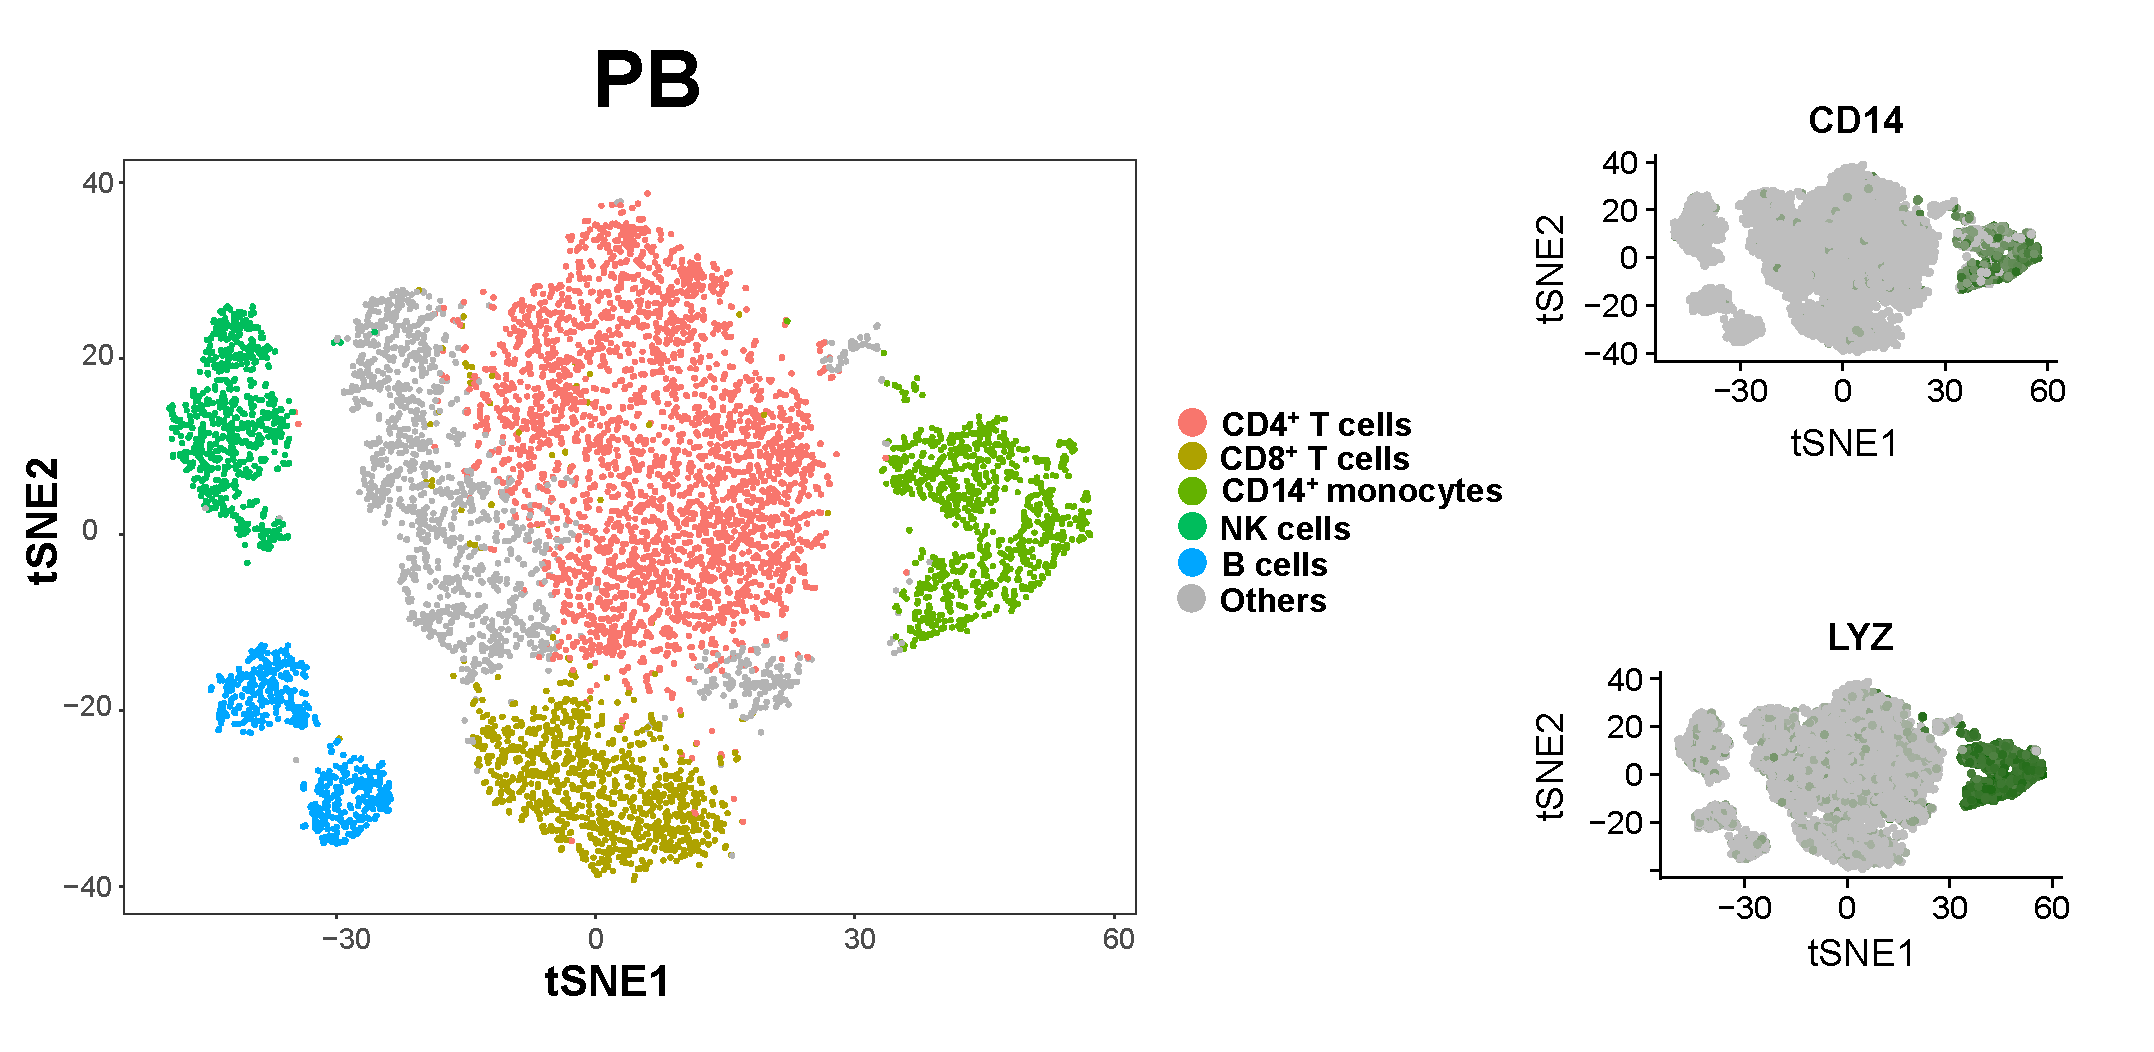
\includegraphics[width=\textwidth]{./Appendix/pdfs/Chapter5/PSA_PB_clusters_and_monocytes_markers}
\caption{}
\end{subfigure}
\caption[Identification of the CD14$^+$ monocytes populations from bulk SFMCs and PBMCs using scRNA-seq transcriptomes.]{\textbf{Identification of the CD14$^+$ monocytes populations from bulk SFMCs and PBMCs using scRNA-seq transcriptomes.} Visualisation using t-SNE dimensional reduction of the cell subpopulations identified in a) SFMCs and b) PBMCs and the overlay of CD14$^+$ monocytes characteristic markers (left hand side panel of a and b) for a representative PsA sample. Clustering performed using recommended resolution (res=0.6) allowed to identify CD4$^+$ (pink), CD8$^+$ (khaki), CD14$^+$ monocytes (gree), NK (purple), DCs (blue), B cells (red) and others (grey). On the left hand side panel, expression for two characteristics CD14$^+$ monocytes markers (\textit{CD14} and \textit{LYZ}) used to subset this population (dark green dots) is overlaid on the t-SNE visual representation of all the cells in each of the tissues.}
\label{figure:PsA_scRNAseq_SF_an_PB_monocytes_identification_from_bulk}
\end{figure}


\caption[Identification of two main CD14$^+$ monocytes subpopulations in the SF and PB combined analysis]{\textbf{Identification of two main CD14$^+$ monocytes subpopulations in the SF and PB combined analysis.} a) Visualisation using tSNE dimensional reduction of the two cluster (CC-mixed and CC-IL7R) identified in the combined SF and PB CD14$^+$ monocyte cells using a very conservative resolution (res=0.1) for the unsupervised clustering analysis. Ech of the dots represents a cell, colour-coded by the cluster membership (pink=CC-mixed and turquoise=CC-IL7R). b) Overlap of \textit{IL7R} and \textit{IL32} expression intensities (green) on the t-SNE representation of the SF and PB CD14$^+$ monocytes.\textit{IL32} and \textit{IL7R} gene expression appeared as markers for the CD14$^+$ monocytes from the CC-IL7R cluster.}

\begin{figure}[htbp]
\centering
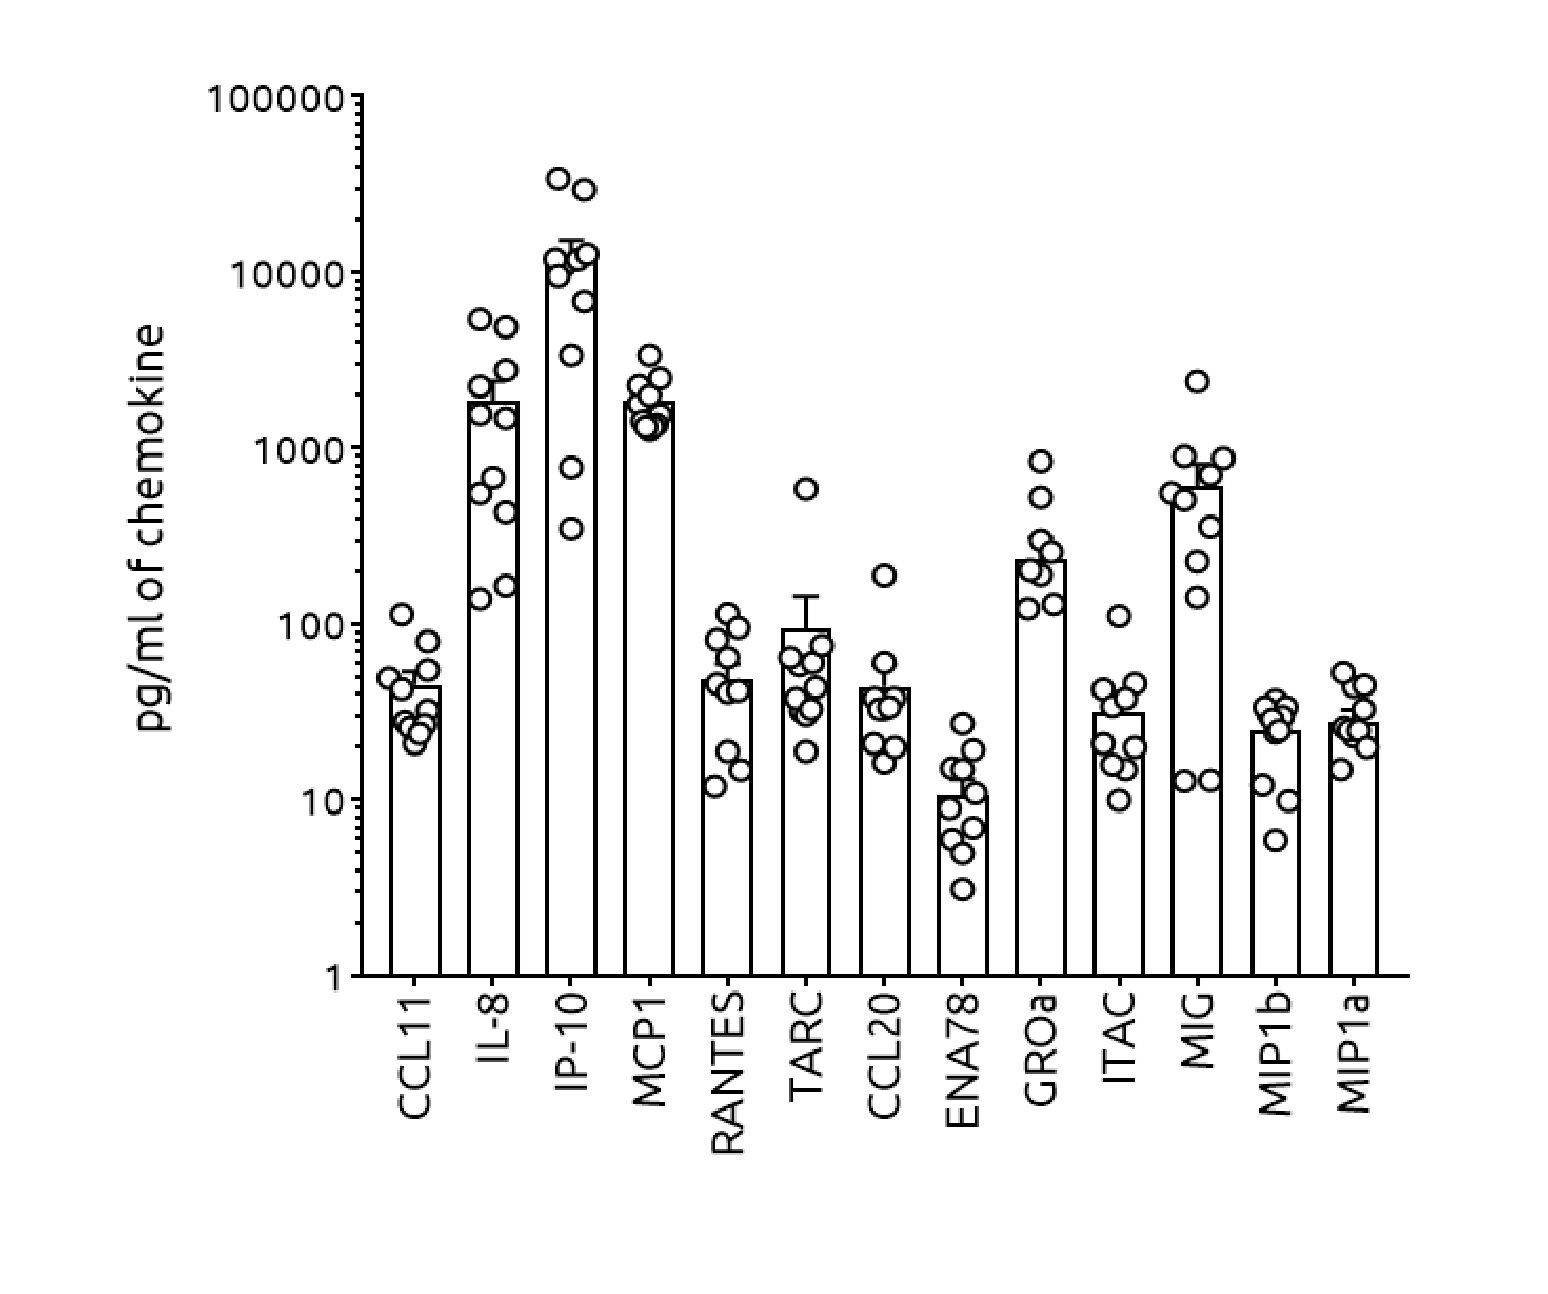
\includegraphics[width=0.5\textwidth]{./Appendix/pdfs/Chapter5/PSA_SF_elisa_cytokines_quantification}
\caption[Quantification of cytokine levels in SF from ten PsA patients.]{\textbf{Quantification of cytokine levels in SF from ten PsA patients.} Barplot graph illustrating pg/mL (x-axis) for a number of cytokines measured from SF of ten PsA patients by collaborators at University xxx using enzyme-linked immunosorbent assay (ELISA). Each circle represents a patients and error bars represent the standard deviation (SD) of the mean from all patients combined. Measurement for the same cytokines was performed in matched plasma from the same patients and all of them failed to be detected.}
\label{figure:ELISA_SF_PsA}
\end{figure}
															%

%\bibliographystyle{abbrvnat2}
%\bibliography{Thesis_ref.bib}

\singlespacing
\setlength\bibitemsep{\itemsep}
\printbibliography
\addcontentsline{toc}{chapter}{Bibliography}

\end{document}

% To count text from latex files http://app.uio.no/ifi/texcount/online.php
% Up to 300 pages for soft binding